% !TEX encoding = UTF-8
% !TEX program = pdflatex
% !TEX spellcheck = it_IT

\documentclass[LaM,binding=0.6cm]{sapthesis}


\usepackage{microtype}
\usepackage[italian]{babel}
\usepackage[utf8]{inputenx}

\usepackage{listings}
\renewcommand{\lstlistingname}{Pseudocode}% Listing -> Pseudocode

\usepackage{color}
\usepackage[usenames,dvipsnames]{xcolor}
\graphicspath{ {./img/} }

\usepackage{hyperref}
\hypersetup{pdftitle={Sviluppo e sperimentazione di algoritmi su grafi in Pregel e Mapreduce},pdfauthor={Luigi Piccioli}} 

%grafici
\usepackage{pgfplots}


% Remove in a normal thesis
\usepackage{lipsum}
\usepackage{curve2e}
\definecolor{gray}{gray}{0.4}
\newcommand{\bs}{\textbackslash}

% Commands for the titlepage
\title{Sviluppo e sperimentazione di algoritmi su grafi in Pregel e Mapreduce}
\author{Luigi Piccioli}
\IDnumber{1434713}
\course{Informatica}
\courseorganizer{Facoltà di Ingegneria dell'Informazione, Informatica e Statistica}
\AcademicYear{2014/2015}
\copyyear{2015}
\advisor{Prof. Irene Finocchi}
%\advisor{Dr. Nome Cognome}
%\coadvisor{Dr. Nome Cognome}
\authoremail{luigipiccioli@gmail.com}

%\examdate{22 Luglio 2015}
%\examiner{Prof. Nome Cognome}
%\examiner{Prof. Nome Cognome}
%\examiner{Dr. Nome Cognome}
\versiondate{\today}




\begin{document}

\frontmatter

\maketitle

%\dedication{Dedicato a\\ Donald Knuth}

%\begin{abstract}
%This document is an example which shows the main features of
%the \LaTeXe\ class \texttt{sapthesis.cls} developed by Francesco Biccari
%with the help of GuIT (Gruppo Utilizzatori Italiani di \TeX).
%\end{abstract}
%
%\begin{acknowledgments}
%Ho deciso di scrivere i ringraziamenti in italiano
%per dimostrare la mia gratitudine verso i membri
%del GuIT, il Gruppo Utilizzatori Italiani di \TeX, e, in particolare,
%verso il prof. Enrico Gregorio.
%\end{acknowledgments}

\tableofcontents

% Do not use the starred version of the chapter command!
%\chapter{Capitolo non numerato}
%
%In this manual you can skip the gray text because it is just dummy text.%
%\footnote{This is a footnote.}
%
%\textcolor{gray}{\lipsum[1-22]}
%
%
%\section*{Paragrafo non numerato}\
%
%In this manual you can skip the gray text because it is just dummy text.
%
%\textcolor{gray}{\lipsum[1-22]}




\mainmatter

\chapter{Introduzione}



MapReduce \cite{Dean:2008:MSD:1327452.1327492} è un modello di programmazione introdotto da Google nel 2008. In pochi anni, questo modello, è stato adottato ed utilizzato da un numero crescente di aziende come Facebook, Yahoo! ed Amazon. Il modello introdotto con MapReduce permette di parallelizzare in modo semplice il calcolo di grandi quantità di dati su di un insieme di macchine.

Negli ultimi anni, con l'espandersi dei social network, l'analisi di grafi di grandi dimensione. Con l'introduzione del modello Pregel \cite{Malewicz:2010:PSL:1807167.1807184} nel 2010, da parte ancora una sempre di Google, viene fornito il modello per il calcolo parallelizzato su un insieme di macchine per grafi di grandi dimensione.

Lo scopo di questo lavoro di tesi è quello di mettere a confronto questi due modelli di programmazione, MapReduce e Pregel, con lo scopo di fornire un analisi sul parallelo delle prestazioni che verranno misurate tramite l'elaborazione di algoritmi su grafi.







\chapter{MapReduce}

\textit{MapReduce} \cite{Dean:2008:MSD:1327452.1327492} è un modello di  programmazione in grado di operare su grandi quantità di dati, dove la computazione viene distribuita e parallelizzata su di un cluster di computer.

Oltre al modello di programmazione, \textit{MapReduce} definisce il modello architetturale del cluster in cui deve essere eseguito il programma. In questo modo sono mantenute separate ed indipendenti le componenti implementative dell'algoritmo \textit{MapReduce} dal framework che si occupa della gestione delle risorse del cluster, del controllo dell'esecuzione del flusso del programma, del controllo degli errori e del recupero successivo al guasto di una o più macchine del cluster.

%L'implementazione di un programma in MapReduce si limita alla definizione della funziona \textbf{MAP} e della funzione \textbf{REDUCE}.

Come rappresentato in Figura \ref{fig:SchemaMapReduce}, il modello suddivide l'esecuzione del programma in due fasi principali: 
	\begin{itemize}
	\item Nella prima, la fase di MAP, i dati di input vengono suddivisi e distribuiti in modo uniforme su di un sottoinsieme di  macchine del cluster, queste macchine eseguono la funzione di MAP che producono dei risultati intermedi in forma di coppie \textit{<chiave,valore>}.
	\item Nella seconda fase, i risultati parziali vengono distribuiti su un secondo sottoinsieme di macchine del cluster, ogni macchina riceve i risultati di tutti i valori intermedi relativi ad una \textit{chiave} e producono un risultato in output.
	\end{itemize}
	
Nelle prossime sezioni di questo capitolo andrò a descrivere più in dettaglio le funzioni che compongono un programma in MapReduce e l'architettura su cui viene eseguito. %TODO riformulare secondo parte

\section{MAP e REDUCE}

Un algoritmo in MapReduce \cite{Dean:2008:MSD:1327452.1327492} è definito attraverso le due funzioni base del modello, la funzione \textbf{MAP} e la funzione \textbf{REDUCE}. 


L'input viene espresso in coppie  di valori \textit{<K,V>} con \textit{K} chiave e \textit{V} il valore associato a \textit{K}.	
Le 2 funzioni base sono definite secondo le seguenti funzioni:
\begin{itemize}
\item \textbf{MAP }	\textit{<K\ped{in},V\ped{in}>} $\Rightarrow$ \textit{list(<K\ped{out},V\ped{out}>)}
\item\textbf{REDUCE}	\textit{<K\ped{in}, list(V\ped{in})>} $\Rightarrow$ \textit{list(V\ped{out})}
\end{itemize}

La funzione di \textbf{MAP} prende in input la coppia di valori \textit{<K\ped{in},V\ped{in}>} e produce in output la lista di valori intermedi \textit{<K\ped{out},V\ped{out}>}, la lista di valori associati alla chiave \textit{K\ped{out}}, che è raggruppata in modo trasparente dal framework \textit{MapReduce} con le liste associate a \textit{K\ped{out}} prodotte dalle altre funzioni \textit{Map} che operano sul cluster.
 
La funzione \textbf{REDUCE} riceve come input una coppia di valori \textit{<K\ped{in},  list(V\ped{in})>} dove \textit{list(V\ped{in})} è l'insieme di tutti valori  associati alla chiave \textit{K\ped{in}} presenti nell'intero input.
La funzione \textit{REDUCE} può restituire in output una lista di valori associati alla chiave \textit{K\ped{in}},\textit{list(V\ped{out})}.

Tra le funzioni \textit{MAP} e \textit{REDUCE} opera, in modo trasparente, la funzione di \textbf{SHUFFLE} la quale raggruppa gli output delle funzioni \textit{MAP}, \textit{list(<K\ped{out},V\ped{out}>)},  che condividono la medesima chiave. Vengono così create le coppie di valori \textit{<K\ped{in}, list(V\ped{in})>} che verranno prese in input dalle funzioni \textit{REDUCE}.

\begin{figure}
\centering
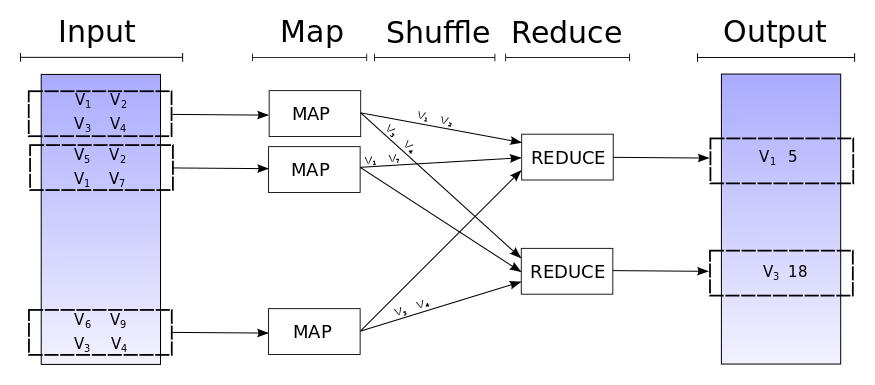
\includegraphics[width=1\textwidth]{esempio_degree}
\caption{Esempio MapReduce - Calcolo del grado dei nodi di un grafo orientato}
\label{fig:SchemaMapReduce}
\end{figure}


\subsection{Esempio MapReduce}

Un esempio di algoritmo in \textit{MapReduce} è il calcolo del grado dei nodi in un grafo orientato, rappresentato in Figura \ref{fig:SchemaMapReduce}. Il questo esempio il grafo in input è rappresentato dalla lista di archi nel formato \textit{<V\ped{a},V\ped{b}>} dove \textit{V\ped{a}} rappresenta il vertice di partenze dell'arco e \textit{V\ped{b}} il vertice di destinazione.

La funzione \textbf{MAP} è la funzione identità. La funzione \textbf{SHUFFLE}, in maniera trasparente, raggruppa le coppie di valori \textit{<V\ped{a},V\ped{b}>} in output da ogni \textit{Mapper} in base al valore chiave \textit{V\ped{a}} e lo instrada verso la funzione \textbf{REDUCE}, garantendo che tutti gli archi di un vertice \textit{V\ped{a}} vengano presi in input dalla stessa funzione \textbf{REDUCE}.

La funzione \textbf{REDUCE} riceve in input la coppia di valori \textit{<V\ped{a}, [V\ped{b1}, V\ped{b2}, … , V\ped{bn}]>}, dove \textit{V\ped{a}} e la chiave del vertice  e \textit{[V\ped{1}, V\ped{2}, … , V\ped{n}]} è l'insieme nodi adiacenti al nodo \textit{V\ped{a}}. La funzione produce in output la coppia \textit{<V\ped{a}, degree(V\ped{a})>} dove degree(V\ped{a}) è il grado del nodo \textit{V\ped{a}} dato dalla cardinalità dell'insieme di nodi [V\ped{b1}, V\ped{b2}, … , V\ped{bn}].
 
\lstdefinestyle{customc}{
  belowcaptionskip=1\baselineskip,
  breaklines=true,
  frame=L,
  xleftmargin=\parindent,
  language=C,
  showstringspaces=false,
  basicstyle=\footnotesize\ttfamily,
  keywordstyle=\bfseries\color{green!40!black},
  commentstyle=\itshape\color{purple!40!black},
  identifierstyle=\color{blue},
  stringstyle=\color{orange},
}
\begin{minipage}{\linewidth}
\lstinputlisting[style=customc,caption={Pseudocodice funzione \textbf{MAP}}]{code/esempioMap.c}
\end{minipage}

\begin{minipage}{\linewidth}
\lstinputlisting[style=customc,caption={Pseudocodice funzione \textbf{REDUCE}}]{code/esempioReduce.c}
\end{minipage}

\section{Architettura MapReduce}

In questo paragrafo viene descritta l'architettura definita in \textit{MapReduce} \cite{Dean:2008:MSD:1327452.1327492} per la gestione del flusso del programma sul cluster di computer.

Il modello dell'architettura \textit{MapReduce} è composto da un nodo \textbf{Master} che si occupa della gestione del flusso dei dati e dell'assegnazione dei \textit{task} a  tutti i nodi del cluster, i \textbf{Worker}.
Il \textit{Master}  può assegnare ai singoli \textit{Worker}, funzioni di \textit{MAP}, in questo caso il \textit{Worker} viene definito \textit{Mapper}, o funzioni \textit{REDUCE}, in questo caso viene definito \textit{Reducer}.

\subsection{Flusso di un programma MapReduce}

In Figura \ref{fig:strutMR} viene rappresentato lo schema del flusso di programma eseguito su l'architettura \textit{MapReduce}. Quando viene inviata un operazione MapReduce al cluster, il flusso del programma segue sette passi:

\begin{enumerate}
\item L’input del programma viene suddiviso in N parti distinte aventi la stessa dimensione.
\item Le copie del programma vengono distribuite a tutte le macchine del cluster (sia Master che Worker)
\item Il Master controlla quali worker si trovano in uno stato IDLE ed assegna loro i task Map e Reduce
\item I Worker che ricevono un task MAP caricano una delle N parti dell'input, leggono le coppie <Key,Value> e salvano nella memorie locali i risultati intermedi generati.
\item I risultati salvati localmente vengono ripartiti utilizzando la funzione di partizione.
\item Il nodo Master riceve la posizione dei risultati partizionati e la comunica ai Reducer a cui sono assegnate la partizioni
\item I Reducer caricano i dati di una partizioni dalle memorie locali dei Mapper, una volta caricati tutti i dati relativi ad una partizione eseguono la funzione REDUCE e producono in output i risultati.
\end{enumerate}
Al termine dell'elaborazione, il programma \textit{MapReuduce} genera \textit{R} file di output, dove \textit{R} è il numero di \textit{Reducer} che sono stati utilizzati.


\begin{figure}
\centering
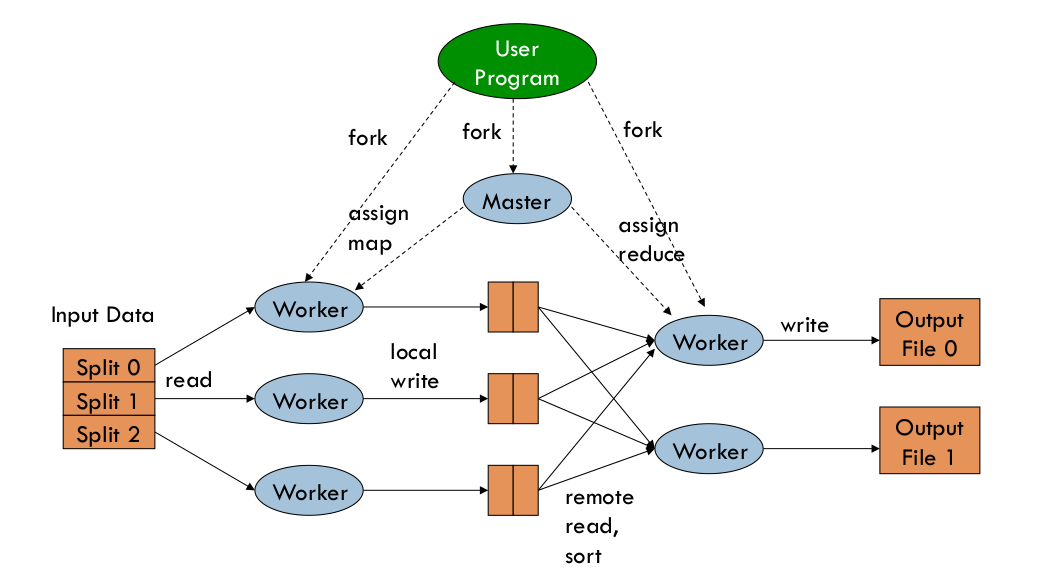
\includegraphics[width=1\textwidth]{esempio_architettura} 
\caption{Archiettetura MapReduce - Flusso di un programma \ref{asd}}%TODO aggiungere rif o cambiare img
\label{fig:strutMR}
\end{figure}


\subsection{Funzione di Partizione}

Per assicurare che ogni \textit{Reducer} ottenga tutti i risultati parziali relativi ad una chiave, prodotti dai \textit{Mapper}, viene utilizzata una funzione di partizione unica. In questo modo lo spazio delle chiavi è ripartito in modo uniforme sia dal \textit{Master} che dai \textit{Worker} del cluster.
Un esempio di funzione di partizione di base utilizzata in \textit{MapReduce} \cite{Dean:2008:MSD:1327452.1327492} è:
\begin{equation*}
	hash(key) / mod R 
\end{equation*}
dove \textit{R} è il numero di partizioni, che solitamente è uguale al numero di \textit{Reducer}.

Nel esempio precedente, dove è calcolato il grado dei nodi di un grafo orientato, applicare la funzione di partizionamento \textit{hash(V\ped{a}) mod R} assicura che tutti le coppie di valori \textit{<V\ped{a} , V\ped{b}>} con chiave \textit{V\ped{a}} vengano assegnate, da tutti i \textit{Worker}, alla stessa partizione.

\subsection{Master}

Il nodo \textit{Master} del cluster si occupa di assegnare e controllare lo stato del progresso dei \textbf{Task}, Map o Reduce, da far svolgere ai \textit{Worker}.

Gli stati in cui possono trovarsi i task sono:
\begin{enumerate}
\item \textbf{Idle}, il task non è stato ancora assegnato a nessun worker
\item \textbf{In-progress}, il task è stato assegnato ed è in esecuzione presso il worker associato
\item \textbf{Completed}, il nodo ha terminato il task assegnato.
\end{enumerate}
Inizialmente tutti i task che compongono il programma MapReduce si trovano in uno stato \textbf{Indle}. Il nodo \textit{Master} verifica la disponibilità delle risorse sui vari \textit{Worker} ed assegna i Task, che passano allo stato \textbf{In-progress}

Appena un task \textbf{Map} passa ad uno stato \textbf{Completed}, il \textit{Master} viene informato della posizione dei risultati parziali che sono stati generati dal \textit{Mapper}. I risultati parziali vengono salvati momentaneamente all'interno della memoria locale del \textit{Mapper}. Il nodo \textit{Master} notifica la posizione di memoria ricevuta, appena possibile, ai \textit{Reducer} a cui è associata la partizione. 
I processi \textbf{Reduce} iniziano ad eseguire la funzione \textit{Reduce} non appena tutti i task \textit{Map} passano ad uno stato \textit{Completed}, significando che  l'intero input è stato letto e partizionato.
Una volta che lo stato di tutti i task \textit{Reduce} passano allo stato \textit{Completed}, l'output del programma è stato salvato su file system distribuito ed il Master termina con successo la computazione.

\subsection{Controllo e gestione degli errori}

MapReduce \cite{Dean:2008:MSD:1327452.1327492} per essere in grado di parallelizzare il processo su cluster composti anche da migliaia di macchine, è essenziale la fase di controllo costante del corretto funzionamento di ogni componente cluster coinvolto nel processo.

Il nodo \textit{Master} si occupa di verificare che i \textit{Worker} siano attivi attraverso l'invio di ping ad intervalli regolari.
Nel caso in cui il \textit{Master} non riceva risposta da uno dei nodi \textit{Worker}, il nodo viene marchiato come \textbf{fallito}.Il fallimento di un nodo causa la riassegnazione e la rielaborazione di alcuni task assegnati al nodo fallito, in modo più dettagliato:
\begin{itemize}
\item{I task \textit{Map} completati nel momento in cui un nodo risulta essere fallito, vengono riportati allo stato iniziale \textit{indle}, in attesa di essere riassegnati ad un altro \textit{Mapper}. La rielaborazione di un task \textit{Map} già completato è necessaria in quanto il fallimento della macchina potrebbe rendere inaccessibile i risultati parziali ai \textit{Reducer}.
}
\item{I task \textit{Map} e \textit{Reduce} che si trovano in uno stato \textit{In-progress} vengono riportati allo stato iniziale \textit{indle}, in attesa di essere riassegnati ad un altro \textit{Mapper} o ad un altro \textit{Reducer}.}
\item{I task \textit{Reduce} che hanno raggiunto lo stato \textit{Completed} non sono influenzati dal fallimento del nodo a cui erano assegnati in quanto il loro output non è salvato in locale ma su file system distribuito.}
\end{itemize}

Il fallimento del nodo \textit{Master} causa il fallimento del programma \textit{MapReduce} e la perdita di tutti i risultati parziali calcolati fino a quel momento.La probabilità che sia il nodo \textit{Master} a fallire è comunque molto bassa rispetto alla probabilità di fallimento di uno dei nodi \textit{Worker}, che possono arrivare a contare anche migliaia di unità.

\section{MapReduce - Iterazioni a cascata}

Non tutti gli algoritmi sono implementabili nel modello MapReduce \cite{Dean:2008:MSD:1327452.1327492} utilzzando una singola iterazione del programma. Per implementare alcuni algoritmi è necessario eseguire più round MapReduce successivi, ad ogni passaggio l'output ottenuto in un round diventa l'input per il round successivo.


\begin{figure}
\centering
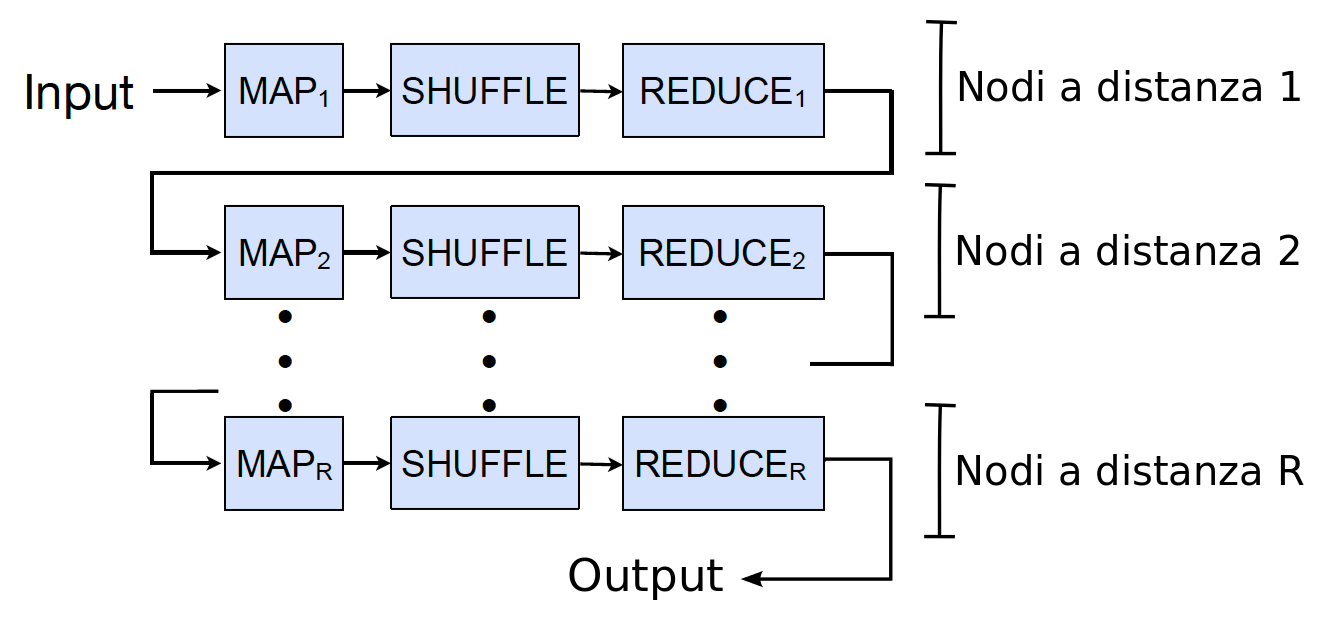
\includegraphics[width=1\textwidth]{MR_cascata}
\caption{MapReduce - Iterazioni a cascata}
\label{fig:MR_cascata}
\end{figure}

In \cite{Karloff:2010:MCM:1873601.1873677} viene descritta la classe di complessità degli algoritmi \textit{MapReduce}, \textbf{\textit{MRC\ap{ i}}}. 
Gli algoritmi che appartengono alla classe \textit{MRC\ap{ i}} devono rispettare una serie di vincoli che limitano la complessità delle funzioni Map e Reduce e del numero di macchine utilizzate, rispetto alla dimensioni dell'input e viene definita in rapporto al numero di round R eseguiti, con \textit{R = O(log\ap{i} n)}.

Nell'esempio visto precedentemente, il calcolo dei nodi di un grafo orientato, viene eseguito in un solo round \textit{MapReduce}.Il numero di iterazioni totali è costante ed uguale a 1 = log\ap{0}n, l'algoritmo appartiene quindi alla classe \textit{MRC\ap{ 0}}.	

Il numero di iterazioni è un fattore importante ed influenza le complessità dell'algoritmo \textit{MapReduce} in quanto al crescere del numero di round aumentano il numero di operazione Shuffle, la quale risulta un'operazione molto costosa.

\textbf{Shuffle}, cioè la funzione che viene svolta in modo trasparente dal modello MapReduce \cite{Dean:2008:MSD:1327452.1327492}, ordina l'output di ogni \textit{Mapper}, lo ripartisce e lo instrada verso il corretto \textit{Reducer}. In questa fase vengono notificate le posizioni dei risultati parziali al nodo \textit{Master}, in questo modo viene introdotto un collo di bottiglia che rende costosa la fase di \textit{Shuffle}. Questo comporta che all'aumentare delle iterazioni \textit{MapReduce} si ha un aumento della complessità del programma. Inoltre ad ogni iterazione si ha un ripetersi delle operazioni di lettura e scrittura dei dati dal file system distribuito, che andranno ad incidere negativamente sulle prestazioni totali.

Un esempio di algoritmo  su grafi, che richiede un implementazione \textit{MapReduce} con più iterazioni, è il calcolo della distanza dei nodi di un grafo da un nodo sorgente, \textit{Single Source Shortest Path (SSSP)}.Quest'ultimo verrà introdotto in modo più dettagliato nel corso del 4° capitolo..

\textit{SSSP}, ad ogni iterazione prende in input la lista di archi del grafo nel formato \textit{<a:dist\ped{a}, b:dist\ped{b}>}, dove \textit{dist} rappresenta la distanza dal nodo sorgente; il valore \textit{dist} è inizializzato nel corso del primo round ad $\infty$ per tutti i nodi ad eccezione del nodo sorgente, il cui valore \textit{dist} è inizializzato a 0.

La funzione \textbf{Map} prende la coppia valori 
\textit{<a:dist\ped{a}, b:dist\ped{b}>}
e produce in output la coppia 
 \textit{<a:dist\ped{a}, b:dist\ped{b}>}.
 
La funzione \textbf{Reducer} riceve la lista dei nodi vicini del nodo nel formato 
\textit{<a:dist\ped{a}, [b\ped{1}:dist\ped{b1},b\ped{2}:dist\ped{b2},... , b\ped{n}:dist\ped{bn} ]>}
e aggiorna i valori\textit{ distanza\ped{bi}} dei nodi vicini, con \textit{i = 1,...,n} con il valore minore tra il valore \textit{dist\ped{bi}} vicini e il valore \textit{dist\ped{a} + 1}, più precisamente:

\begin{minipage}{\linewidth}
\lstinputlisting[style=customc,caption={Pseudocodice funzione \textbf{Reduce} SSSP}]{code/esempioSSSPreduce.c}		
\end{minipage}

Le iterazione MapReduce terminano quando l'algoritmo converge e non avvengono più modifiche ai valori distanza.

\section{Implementazioni MapReduce}


Esistono numerosi framework che implementano e/o includono il modello MapReduce \cite{Dean:2008:MSD:1327452.1327492}, tra i più utilizzati troviamo: 
\begin{itemize}
\item Apache Hadoop \cite{1_hadoop.apache.org_2015}.
\item Google MapReduce \cite{Dean:2008:MSD:1327452.1327492}.
\item MongoDB \cite{2_mongodb.org_2015}.
\item Aster Data \cite{3_it.teradata.com_2015}.
\end{itemize}


Per l'implementazione di algoritmi su grafi in MapReduce, in questo lavoro di Tesi è stato utilizzato Apache Hadoop, essendo la soluzione Open Source più utilizzata e meglio documentata.

Questa scelta permette un confronto più diretto degli algoritmi sviluppati su Apache Giraph \cite{4_giraph.apache.org_2015} , un framework che implementa il modello Pregel \cite{Malewicz:2010:PSL:1807167.1807184}, sviluppato integrandolo su Apache Hadoop e che verrà approfondito nel prossimo capitolo.

Le componenti principali, vedi \ref{fig:layer_hadoop} , di Apache Hadoop sono :
\begin{itemize}
\item \textbf{Hadoop Distributed File System (HDFS)}: File system distribuito
\item \textbf{Hadoop YARN,  Yet Another Resource Negotiator}: A framework per la gestione gestione delle risorse del cluster.
\item \textbf{Hadoop MapReduce}:  Implementazione del modello MapReduce
\end{itemize}

\begin{figure}
\centering
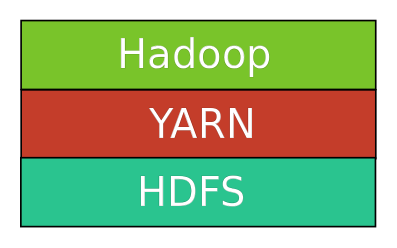
\includegraphics[width=0.5\textwidth]{layer_hadoop}
\caption{Architettura Apache Hadoop}
\label{fig:layer_hadoop}
\end{figure}

Ogni programma implementato in \textit{Apache Hadoop} istanzia uno o più \textbf{Job}, cioè programmi che seguono il modello MapReduce. La definizione di un \textit{Job} è suddiviso in 2 parti, la configurazione del cluster e l'implementazione delle funzioni di \textit{Map} e di \textit{Reduce}. 
La configurazione del cluster su cui verrà eseguito il Job prevede, per esempio, la definizione del numero di \textit{Mapper} e \textit{Reducer} che verranno utilizzati. 
\textbf{Hadoop MapReduce} si occupa della gestione del flusso del Job, lo divide in sotto-parti, i task, che verranno assegnati ai Worker presenti cluster, i Container.
Le risorse del Cluster vengono gestite da \textbf{Hadoop YARN} che istanzia, a seconda delle disponibilità delle risorse sulle singole macchine, i \textit{Container}. I container sono le entità che andranno a eseguire i \textit{task} assegnati.
\textbf{Hadoop Distributed File System} è l'implementazione di file system distribuito associato alla distribuzione Apache Hadoop, utilizzato dai \textit{Mapper} per caricare i dati dell'input e dai \textit{Reducer} per scrivere l'output. In Figura \ref{fig:layer_hadoop} è rappresentata l'architettura di Apache Hadoop.



\chapter{Pregel}

Il modello \textbf{Pregel} \cite{Malewicz:2010:PSL:1807167.1807184}  è  un modello per l'esecuzione distribuita, parallelo e fault-tolerant di algoritmi su grafi su cluster di computer.
\textit{Pregel} può essere definito come una specializzazione di MapReduce \cite{Dean:2008:MSD:1327452.1327492} sui grafi.
Come avviene in \textit{MapReduce} il modello è composto sia dalla specifica dell'architettura su cui eseguire il programma sia dalla specifica del modello di programmazione, in modo da mantenere separate ed indipendenti le due parti. 


Un programma  sviluppato in \textit{Pregel} permette di definire algoritmi su grafi in modo più intuitivo rispetto a \textit{MapReduce}, inoltre permette di evitare i costi delle numerose operazioni di I/O e delle operazioni di Shuffle, viste nel capitolo precedente. Questi costi sono evitati perché non è più presente l'inefficienza causata dalla presenza di molteplici iterazioni dell'algoritmo, iterazioni spesso necessarie per l'implementazione di algoritmi su Grafi, come nell'esempio di SSSP visto nel capitolo precedente. 

Un programma, sviluppato secondo il modello definito in Pregel, viene definito attraverso la funzione \textit{compute}, che definisce la logica del programma dal punto di vista del vertice del grafo. Ad ogni iterazione S del programma (chiamato Superstep) con S = 0,1,2.. , un vertice in Pregel:
\begin{itemize}
\item Riceve i messaggi inviati durante il Superstep \textit{S-1}, l'iterazione Pregel precedente.
\item Invia i messaggi ad altri vertici del grafo, che verranno ricevuti nel Superstep successivo \textit{S+1}.
\end{itemize}

\section{Bulk Synchronous Parallel (BSP)}
\textit{Pregel} si basa sul modello descritto in \cite{Valiant:1990:BMP:79173.79181}, il\textbf{ Bulk Synchronous Parallel (BSP)}.
\textit{BSP }è un modello computazionale astratto per la progettazione di algoritmo paralleli.Una macchina \textit{BSP} è costituita da più processori, ognuno avente la propria memoria locale indipendente e connessi tra loro da una rete di comunicazione.

Una computazione definita secondo \textit{BSP} è composta da una serie di Superstep globali, ogni Superstep è composto da:
\begin{itemize}
\item \textbf{Calcolo concorrente}: Ogni processore che partecipa al Superstep effettua le operazioni utilizzando la propria memoria locale.
\item \textbf{Comunicazione}: In questa fase i processori scambiano dati tra loro.
\item \textbf{Barriera di sincronizzazione}: Un processo che raggiunge questo step, rimane in stato di attesa fino a quando tutti i processi non hanno terminato la fasi precedenti.
\end{itemize}

La \textit{Barriera di sincronizzazione} evita che si creino dipendenze circolari, rendendo impossibile il deadlock dei processi in \textit{BSP}, inoltre permette l'implementazione di Checkpoint per la gestione di errori dovuti a fallimenti di una o più macchine che compongono il cluster. L'utilizzo della \textit{Barriera di Sincronizzazione} può portare a conseguenze potenzialmente molto costose, basti a pensare ad un processo che richiede un tempo maggiore rispetto agli altri processi e provoca la permanenza prolungata di questi ultimi nello stato di attesa. Per evitare questo fenomeno è molto importante che ogni processore esegua le stesse funzioni su quantità di dati simili.

\begin{figure}
\centering
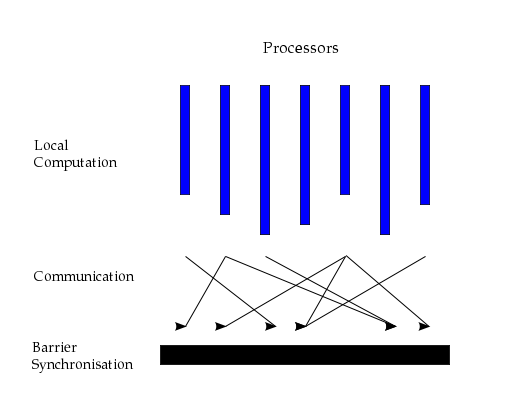
\includegraphics[width=1\textwidth]{BSP}
\caption{Bulk Synchronous Parallel (BSP) \cite{1_wikipedia_2015}}
\label{fig:BSP}
\end{figure}

La computazione di un programma definito in \textbf{Pregel} \cite{Malewicz:2010:PSL:1807167.1807184} è suddivisa in Superstep. Ad ogni \textit{Superstep} viene eseguita la funzione \textit{Compute} che può prevedere la ricezione e l'invio di messaggi da e verso altri vertici del grafo. Come mostrato in Figura \ref{fig:msPregel}, un Superstep termina quando tutti i vertici del grafo hanno completato la funzione \textit{Compute} e si trovano in uno stato \textit{Inattivo}.

\section{Pregel}

Il modello \textbf{Pregel} viene definito come un modello di computazione \textit{vertice-centrico} su grafi diretti. 
La struttura di un vertice \textit{V} in \textit{Pregel} è composta da:
\begin{itemize}
\item \textbf{ID vertice}: Una stringa che identifica univocamente il vertice \textit{V} sul grafo.
\item \textbf{Stato del vertice}: Un valore mutabile durante l'esecuzione associata al vertice \textit{V}.
\item \textbf{Lista di archi uscenti}: L'insieme degli archi diretti che hanno il vertice \textit{V} come nodo sorgente.
\end{itemize}
Gli archi in \textit{Pregel} sono entità secondarie e sono associate alla struttura del vertice sorgente dell'arco. La struttura di un arco è composto da un valore mutabile durante l'esecuzione del Superstep e dall'identificativo del nodo di destinazione dell'arco.

Un programma  in \textit{Pregel} è costituito da tre fasi principali: 
\begin{itemize}

\item Nella prima fase viene caricato lo stato iniziale del grafo di input, per esempio da un file system distribuito. 
\item Nella seconda fase vengono eseguiti una serie di Superstep necessari all'esecuzione dell'algoritmo. Durante il Superstep, i vertici eseguono tutti la stessa funzione sulla struttura del vertice. Tale funzione definisce la logica dell'algoritmo.
\item Nell'ultima fase viene scritto l’output del programma. 
\end{itemize}
La terminazione dell'algoritmo è raggiunta quando tutti i vertici si trovano in uno stato \textit{Vote to Halt}. Nel primo Superstep, tutti i vertici si trovano nello stato \textit{Active}, ad ogni Superstep il vertice può  passare o meno allo stato \textit{Vote to Halt}.

Un vertice \textit{V} che passa allo \textit{Vote to Halt} nel Superstep \textit{s}, rimane inattivo, cioè non effettua operazioni nei Superstep successivi a \textit{s}. \textit{V} rimane inattivo finché tutti i vertici passano allo stato \textit{Vote to Halt} e viene terminata l’esecuzione del programma oppure, il vertice \textit{V},  riceve un messaggio in entrata al Superstep \textit{r} (con \textit{r > s}), questo fa tornare il vertice V ad uno \textit{Active}, quindi a riprende le operazioni previste nel corso del Superstep \textit{r}.

Nella Figura \ref{fig:msPregel} è rappresentata la macchina degli stati di un vertice in Pregel.

\begin{figure}
\centering
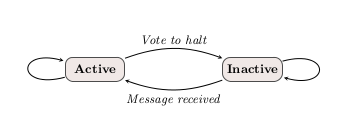
\includegraphics[width=0.5\textwidth]{macchinastatipregel}
\caption{Macchina degli stati di un Vertice in Pregel}
\label{fig:msPregel}
\end{figure}

\subsection{Esempio Pregel}
 
Un esempio base di algoritmo in \textit{Pregel }\cite{Malewicz:2010:PSL:1807167.1807184} è il calcolo del grado uscente dei nodi di un grafo orientato. 
L'implementazione in \textit{Pregel} prevede la definizione di una funzione \textit{Compute()} che implementa le azioni che svolge un vertice nel corso del \textit{Superstep}. L'implementazione dell'algoritmo per il calcolo del nodo del grafo prevede un \textit{Superstep} in cui ogni vertice conta il numero di archi uscenti associati alla propria struttura, assegna al proprio stato il valore associato alla struttura del vertice e passa allo stato \textit{Vote to Halt}.
Tutti i vertici passano allo stato \textit{Vote to Halt} dopo il primo \textit{Superstep}, i vertici salvano il proprio stato su File System Distribuito e il programma termina.

\begin{minipage}{\linewidth}
\lstinputlisting[style=customc,caption={Esempio del calcolo del grado uscente in \textbf{Pregel}}]{code/esempioPregele.c}
\end{minipage}


\section{Architettura Pregel}

Come avviene per \textit{MapReduce} \cite{Dean:2008:MSD:1327452.1327492}, il modello Pregel definisce anche l'architettura del cluster su cui è eseguito il programma, mantenendola separata e indipendente dalla componente in cui viene implementato l'algoritmo.

L’architettura del cluster ha un'organizzazione di tipo \textit{Master - Worker} simile all'architettura descritta in \textit{MapReduce}.
I vertici caricati in input vengono suddivisi tramite una funzione di partizione. Ogni partizione del grafo viene assegnata ad un \textit{Worker}. 

La funzione di partizione di default definita in \textit{Pregel} è la funzione Hash:
\textit{hash(VERTEX ID) \% N}, con N numero di nodi \textit{Worker} nel cluster.

\textit{Pregel} prevede la possibilità di definire una funzione di partizione ad hoc per migliorare la partizione del grafo in modo da distribuire in modo uniforme i costi computazionali su tutti i \textit{Worker}, per esempio il bilanciamento del grado totale dei vertici presenti nelle partizioni assegnate ai \textit{Worker}. Questo permette di poter bilanciare il carico computazionale sui \textit{Worker} adattandolo all'algoritmo da implementare in Pregel.

Il modello definisce inoltre un meccanismo per il coordinamento tra i nodi e per il controllo globale della computazione durante l'esecuzione di un programma \textit{Pregel}. Ad ogni Superstep S, un vertice, può fornire un valore attraverso questo meccanismo, chiamato \textbf{Aggregatore}. L'Aggregatore combina i valori ricevuti e produce un valore aggragato che è reso disponibile a tutti i vertici del Grafo attivi nel Superstep successivo S+1.


\begin{figure}[b]
\centering
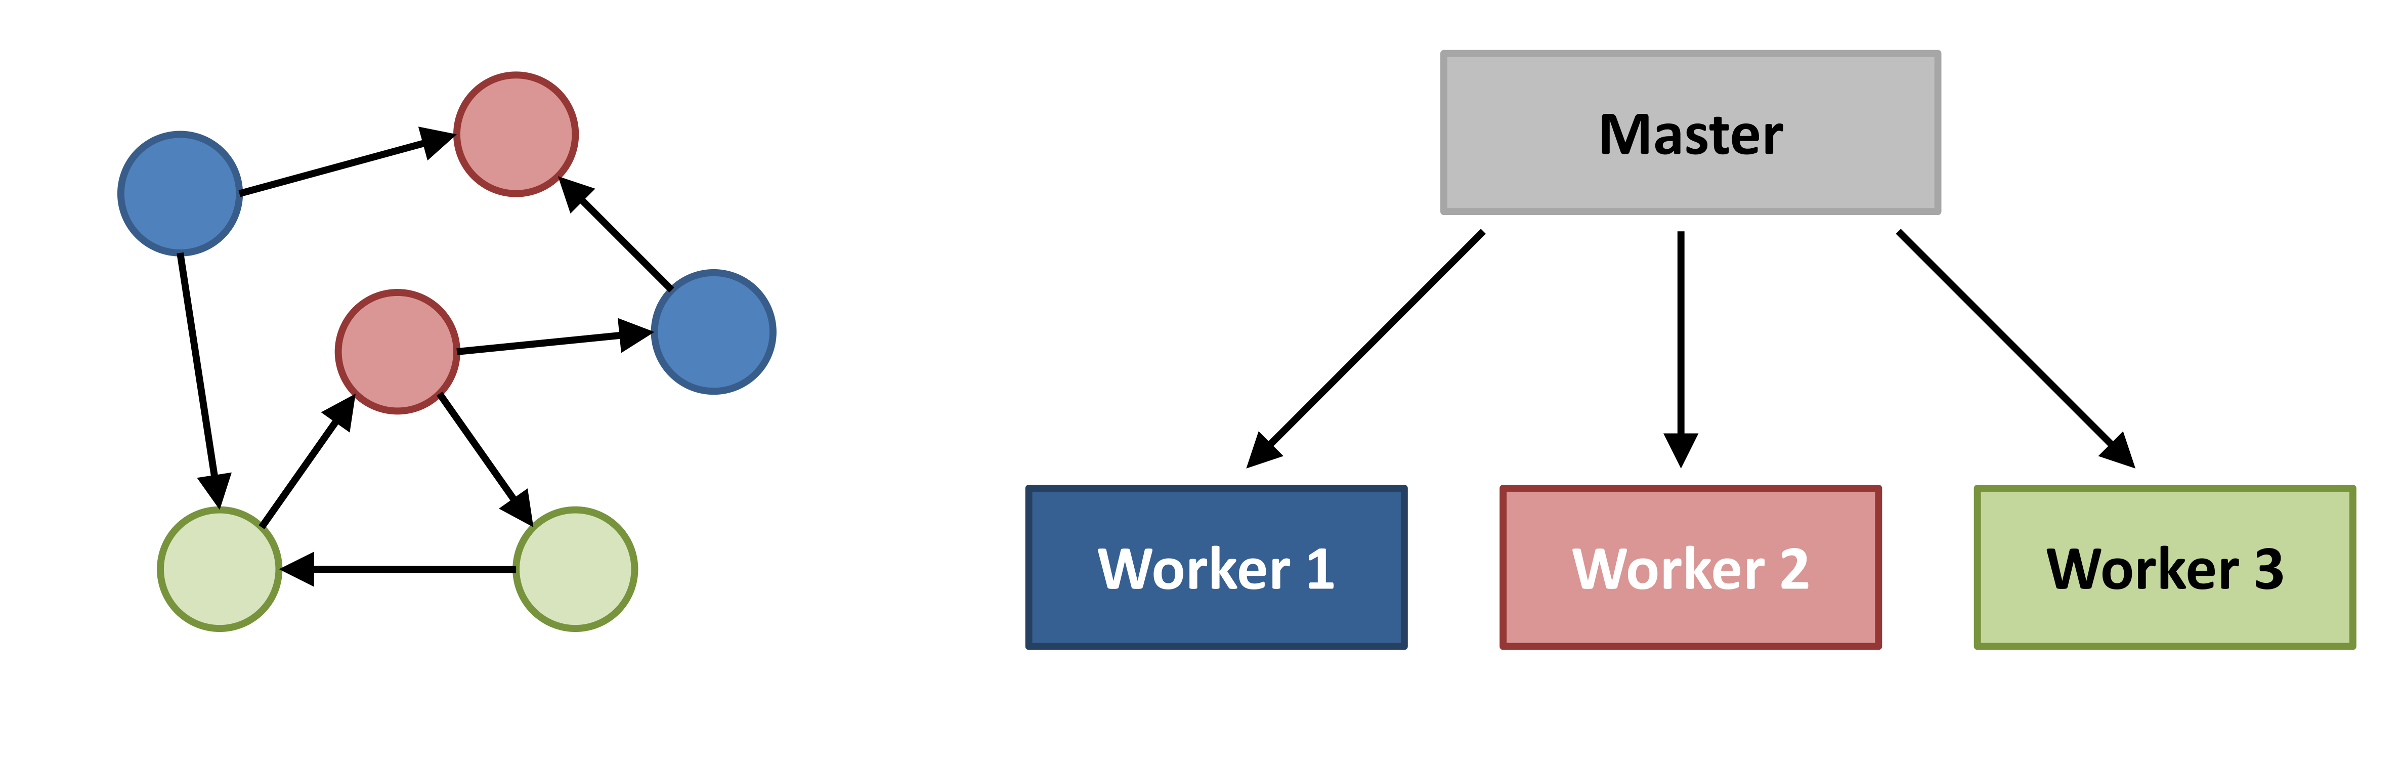
\includegraphics[width=1\textwidth]{partizionePregel}
\caption{Partizionamento vertici in Pregel}
\label{fig:partizPregel}
\end{figure}

\subsection{Flusso di un programma Pregel}

L'esecuzione di un programma Pregel sul cluster segue i seguenti passi:
\begin{itemize}
\item Le copie del programma vengono distribuite a tutti i nodi del cluster, uno dei nodi viene eletto nodo \textit{Master} con il compito di coordinamento dei nodi \textit{Worker}, il nodo \textit{Master }non ha partizioni del grafo assegnate.
\item Il nodo \textit{Master} determina le partizioni del grafo e le assegna ai \textit{Worker}, come  mostrato in Figura \ref{fig:partizPregel}. I \textit{Worker} si occupano di mantenere lo stato della partizione assegnata e di eseguire la funzione \textit{Compute} sui tutti i vertici che appartengono alla partizione. 
\item Il nodo \textit{Master} assegna una porzione dell’input ad ogni \textit{Worker}. I nodi \textit{Worker} leggono la porzione di input assegnato e, nel caso in cui il vertice appartiene a una partizione assegnata allo stesso Worker, creano direttamente la struttura dati del vertice in memoria locale. Se il Vertice in input, invece, appartiene ad una partizione assegnata ad un altro \textit{Worker}, viene inviato un messaggio al \textit{Worker} che creerà la struttura dati del vertice nella propria memoria locale. Finita la fase di caricamento del grafo, tutti i nodi del grado passano allo stato \textit{Active}.
\item Il \textit{Master} comunica a tutti i \textit{Worker} l'inizio del Superstep. I \textit{Worker} eseguono la funzione \textit{Compute()} sui vertici attivi della  partizione assegnatagli, al termine i \textit{Worker} inviano al \textit{Master} il numero di nodi che sono nello stato \textit{Active} nel Superstep successivo. Questo passaggio viene ripetuto finché sono presenti nodi \textit{Active} nel grafo e sono presenti messaggi da recapitare nel \textit{Superstep} successivo.
\item Quando tutti i nodi si trovano nello stato \textit{Vote to Halt} il \textit{Master} comunica ai nodi \textit{Worker} che la computazione è terminata e che è necessario salvare la propria partizione del grafo nell'output.
\end{itemize}

\subsection{Master}

Il nodo \textbf{Master} ha come funzione principale il coordinamento del lavoro dei nodi \textit{Worker}. Il \textit{Master} mantiene una struttura dati locale composta dal numero identificativo di ogni \textit{Worker} attivo e le partizioni assegnate ad ogni \textit{Worker}. 
Non viene mantenuta nessuna informazione riguardante il grafo in input, mantenendo quindi una struttura dati le cui dimensioni sono proporzionali al numero di partizioni del grafo e non al numero di vertici o archi del grafo stesso, permette di poter gestire il coordinamento di grafi di grandi dimensioni.

Le operazioni svolte dal Master seguono lo stesso ciclo di \textit{Superstep} in cui viene suddivisa la computazione del \textit{Worker}.
Ogni volta che viene raggiunta una \textit{Barriera di Sincronizzazione} il \textit{Master} verifica, tramite ping, quali \textit{Worker} sono ancora attivi. In caso non si verificano errori e tutti i \textit{Worker} sono ancora attivi allora il \textit{Master} fa avanzare la computazione al \textit{Superstep} successivo. Se viene rilevato il fallimento di uno o più \textit{Worker} si avvia la procedura di recupero che vedremo più avanti.

Ad ogni ciclo il \textit{Master} si occupa di mantenere una serie di informazioni statistiche sullo stato totale del grafo, come il numero di vertici e archi attivi oppure il numero di messaggi inviati, le informazioni sono raccolte nel corso di un \textit{Superstep }e rese disponibili a tutti i Worker nel \textit{Superstep} successivo.

\subsection{Worker}
I nodi \textbf{Worker} mantengono le strutture dati dei vertici che appartengono alla partizione del grafo assegnatagli durante la fase iniziale dal \textit{Master}. La struttura dati di un vertice è composta dal suo identificativo, dal valore corrente del vertice, dalla lista di messaggi in entrata e dalla lista degli archi uscenti dal vertice; ogni arco è rappresentato dall'indice del vertice di destinazione e dal valore associato all'arco stesso.

Il modello non prevede l'accesso alla lista degli archi in entrata in un nodo, archi che saranno gestiti dai vertici sorgente, Vertici che si potrebbero trovare o all'interno della partizione dello stesso Worker o su una partizione del grafo assegnata ad un Worker differente.

\subsection{Aggregatori}
In \textbf{Pregel }\cite{Malewicz:2010:PSL:1807167.1807184}, gli aggregatori implementano il meccanismo per il calcolo di valori globali. Ogni vertice può inviare un valore al sistema di aggregazione, i valori inviati da tutti i vertici verranno aggregati e resi disponibili dal Superstep successivo. 
\textbf{Pregel} implementa una serie di aggregatori di esempio: MIN per il calcolo del valore minimo, MAX per il calcolo del valore massimo e SUM per la somma totale dei valori passati all'aggragatore
Un esempio di utilizzo dell'aggregatore MAX è calcolo del grado massimo dei vertici di un grafo orientato. Una volta ottenuto il valore del grado uscente del nodo, il valore viene inviato all'aggregatore. Alla fine del \textit{Superstep} i \textit{Worker} raccolgono i valori passati all'aggregatore MAX dai vertici ed ottengono un valore aggregato parziale. 
Ogni \textit{Worker} invia al nodo \textit{Master }il valore aggregato MAX parziale, il \textit{Master }aggraga a sua volta i valori ottenendo il valore aggregato MAX globale, che rappresenta il grado massimo dei vertice del grafo. In Figura \ref{fig:aggPregele} viene mostrato un esempio di aggregatore MAX.

Alla fine del \textit{Superstep}, il \textit{Master} invierà il valore aggregato a tutti i \textit{Worker} che sarà disponibile quindi dal \textit{Superstep} successivo.


\begin{figure}
\centering
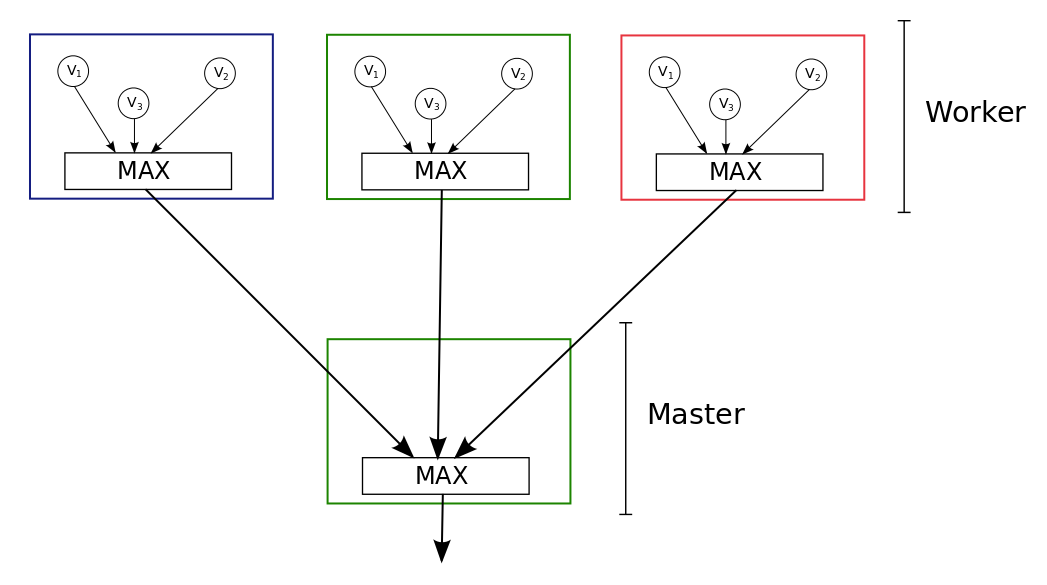
\includegraphics[width=1\textwidth]{disegno_pregel_aggregartori}
\caption{Aggregatore MAX}
\label{fig:aggPregele}
\end{figure}

\subsection{Gestione e recupero degli errori}
Come in \textit{MapReduce}, Pregel è in grado di parallelizzare il processo su cluster composti anche da migliaia di macchine, questo richiede un controllo dello stato di ogni macchina in modo da garantire il funzionamento dell'intera architettura. Il \textit{Master}, come visto, controlla lo stato dei \textit{Worker} tramite un sistema di Ping inviati periodicamente.
Per garantire il recupero dello stato del grafo a seguito di un errore da parte di uno dei \textit{Worker}, all'inizio di alcuni \textit{Superstep}, il \textit{Master }comunica ai \textit{Worker} di salvare sul File System distribuito lo stato della propria partizione. Per non appesantire troppo il processo questa operazione non viene fatta all'inizio di ogni \textit{Superstep} ma a determinati checkpoint stabiliti dal nodo \textit{Master}.

Come mostato in \ref{fig:recovPregele}, quando il \textit{Master} rileva il fallimento da parte di uno o più \textit{Worker} e di conseguenza la perdita dello stato corrente di alcune partizioni del grafo, procede alla riassegnazione delle partizioni appartenenti alle macchine fallite sui nodi \textit{Worker} rimasti attivi.
I \textit{Worker} che ricevono nuove partizioni da gestire, caricano l'ultimo stato della partizione salvate sul file system distribuito.
Il calcolo viene fatto ripartire dal \textit{Superstep} successivo al checkpoint ripristinato, che si riferisce al Superstep successivo all'ultimo salvataggio dello stato del grado.


\begin{figure}
\centering
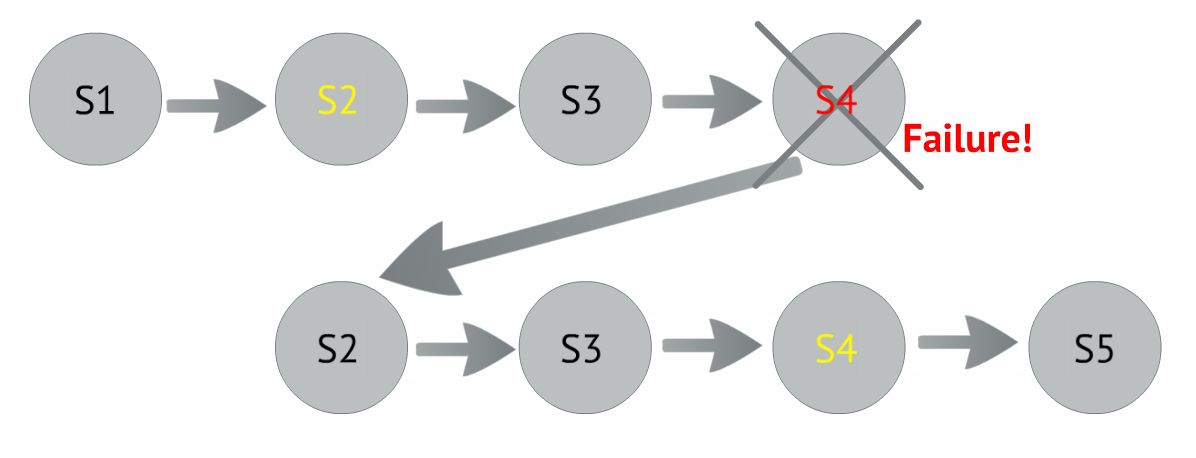
\includegraphics[width=1\textwidth]{giraph-tollerance}
\caption{Checkpoint Pregel}
\label{fig:recovPregele}
\end{figure}

\section{Giraph - Numero di iterazioni}
Algoritmi su grafi che richiedono un numero elevato di iterazioni vengono implementati agevolmente nel modello Pregel, dove ad ogni Superstep viene applicata la logica delle iterazioni richieste.
Al contrario di come avviene in \textit{MapReduce}, il crescere del numero non aumenta la complessità del algoritmo, anzi la progettazione di algoritmi in \textit{Pregel} è basata su azioni eseguite in una serie di iterazioni sul grafo.

Un esempio con più iterazioni è l'implementazione \textit{Pregel} di \textit{SSSP}, introdotto nel capito precedente e che verrà descritto più dettagliatamente nel capitolo successivo. In \textit{SSSP }il valore associato ad ogni vertice è inizializzato ad $\infty$ per tutti i nodi tranne per il nodo sorgente, inizializzato con valore 0, questi valori rappresentano la distanza minima dei nodi dal nodo sorgente.

La logica da applicare al singolo vertice nel corso di un Superstep è:

\lstinputlisting[style=customc,caption={Esempio \textbf{Pregel}}]{code/esempioPregeleSSSP.c}


Nel \textit{Superstep S} il vertice \textit{V }riceve il valore \textit{distanza minima} tramite un messaggio dai vertici a cui si trova vicino. Confronta le distanze ricevute con il proprio valore \textit{distanza minima} attuale e lo aggiorna nel caso un nodo a cui si trova vicino sia a distanza minore dal nodo sorgente.
Quando tutti i vertici, al termine di un \textit{Superstep}, si trovano nello stato \textit{Vote to Halt}, significa che nessun vertice ha aggiornato il proprio valore \textit{distanza minima} nel corso dell'ultimo \textit{Superstep} e il programma termina. 



\section{Implementazioni Pregel}
Sono stati sviluppati diversi framework che implementano il modello Pregel \cite{Karloff:2010:MCM:1873601.1873677}, tra cui:
\begin{itemize}
\item Apache Giraph \cite{4_giraph.apache.org_2015}
\item GPS\cite{5_infolab.stanford.edu_2015}
\item Google Pregel \cite{Malewicz:2010:PSL:1807167.1807184}
\item GraphLab \cite{6_dato_2015}
\end{itemize}

in \cite{Han:2014:ECP:2732977.2732980} sono stati confrontati tra loro i framework, analizzando le prestazioni dei vari sistemi su diversi algoritmi su grafi, come SSSP e PageRank, applicandoli su grafi di diverse dimensioni.
Nel lavoro viene mostrato come i due sistemi, Apache Giraph e GPS, ottengono prestazioni migliori rispetto agli altri sistemi confrontati. Tra questi due framework si è deciso di utilizzare per Apache Giraph che è la soluzione OpenSource più documentata, meglio sviluppata e largamente supportata della comunità.


\begin{figure}
\centering
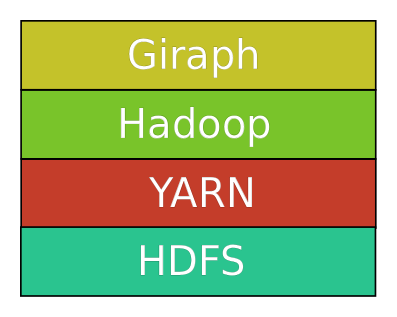
\includegraphics[width=0.5\textwidth]{layer_giraph}
\caption{Apache Giraph}
\label{fig:giraph}
\end{figure}

Un altro fattore  che ha inciso sulla decisione di scegliere Apache Giraph come sistema di testing per il modello Pregel è il fatto che il framework è sviluppato integrandolo direttamente sulla infrastruttura di Apache Hadoop, questo ha reso possibile effettuare un confronto più diretto e preciso delle qualità prestazionali tra due sistemi.

\chapter{Algoritmi implementati}

Il confronto tra i Modelli \textit{MapReduce} \cite{Dean:2008:MSD:1327452.1327492} e Pregel \cite{Malewicz:2010:PSL:1807167.1807184} è stato effettuato mettendo a confrono le loro implementazioni più utilizzate, rispettivemente \textit{Apache Hadoop} \cite{1_hadoop.apache.org_2015}e \textit{Apache Giraph} \cite{4_giraph.apache.org_2015}.
Per questo lavoro di tesi sono stati selezionati cinque algoritmi su grafi e messe a confronto le rispettive implementazioni sui due modelli studiati. Degli algoritmi selezionati, quattro algoritmi sono applicati a grafi non orientati e un algoritmo su grafi orientati. Gli algoritmi per grafi non orientati sono:
\begin{enumerate}
\item \textbf{DegreeCalculator}, Calcolo del grado dei vertici.
\item \textbf{SSSP}, Cammini minimi da sorgente singola.
\item \textbf{NodeIterator++} \cite{Suri:2011:CTC:1963405.1963491} , Algoritmo per il calcolo dei triangoli presenti nel grafo.
\item \textbf{Densest Subgraph} \cite{DBLP:journals/corr/abs-1201-6567}, Algoritmo per la ricerca del sottografo più denso del grafo, nella sua versione per grafi non orientati.
\end{enumerate}

Per i grafi orientati invece è stata sviluppata la versione dell'algoritmo \textbf{Densest Subgraph} \cite{DBLP:journals/corr/abs-1201-6567} nella versione per grafi diretti.

Il modello \textit{Pregel}, come visto nel terzo capitolo, è sviluppato a partire da grafi orientati, dove ogni arco del grafo è associato alla struttura dati del vertice sorgente. Per la rappresentazione di grafi non orientati, in Pregel, e necessario rappresentare gli archi del grafo non orientato da coppie di archi, uno per ogni direzione. Quindi un arco non orientato \textit{(u,v)} è rappresentato dalla coppia di archi orientati \textit{(u,v) }e \textit{(v,u)}, la prima coppia associata al vertice \textit{v} mentre la seconda al vertice \textit{u}.
Per questo motivo, le implementazioni degli algoritmi su grafi non orientati sono stati sviluppati partendo da un input composto da entrambe le coppie orientate che formano il grafo non oriento.

Per i test è stata necessaria l'implementazione di quasi tutti gli algoritmi scelti. Per l'algoritmo \textit{SSSP} è stata utilizzata l'implementazione per grafi orientati presente nel package \textit{giraph-examples} all'interno della disribuzione del framework \textit{Apache Giraph} \cite{4_giraph.apache.org_2015}.
Per  NodeIterator++ è stata utilizzata l'implementazione dell'algoritmo in MapReduce in \textit{Apache Hadoop} \cite{1_hadoop.apache.org_2015} implementata in \cite{DBLP:journals/corr/FinocchiFF14}.
 
In questo capitolo, per ognuno dei cinque algoritmi verrà fornita una descrizione generale dei passi dell'algoritmo ed una descrizione dell'implementazione per i modelli \textit{MapReduce} e \textit{Pregel}.

%Le prestazioni ottenute dalle verranno poi descritte e confrontate nel capitolo successivo.


\section{DegreeCalculator}

L'algoritmo per il calcolo del grado dei nodi, prende in input un Grafo non orientato \textit{G = (V,E)} dove\textit {V} sono i vertici del grafo \textit{G} ed \textit{E} sono gli archi del grafo \textit{G}. Per ogni nodo \textit{$v \epsilon V$} l'algoritmo calcola il grado del vertice \textit{deg(v)}, con  \textit{deg(v)=|\{(v,u)|$(v,u) \epsilon E$\}|}.

\subsection{MapReduce}

L'algoritmo \textit{DegreeCalculator} è stato implementato in una iterazione \textit{MapReduce}, rappresentata in Figura \ref{fig:MRDEGREE}.

La funzione \textit{Map}, come mostrato nello pseudocodice \ref{lst:esMap} , è la funzione identità, prende in input la coppia di valori \textit{<v,u>} che rappresenta un arco del grafo e restituisce in output la coppia \textit{<v,u>}.

La funzione \textit{Reduce} riceve in input la coppia di valori \textit{<v, list(u)>} dove \textit{list(u)} è la lista  di vertici adiacenti al vertice \textit{v}. La funzione \textit{Reduce} restituisce in output la coppia di valori \textit{<v,degree(v)>} dove \textit{degree(v)} è il grado del nodo \textit{v} dato dal numero di vertici presenti in \textit{list(u)}. In \ref{lst:esReduce} è mostrato lo pseudocodice della funzione \textit{Reduce}.

\begin{minipage}{\linewidth}
\lstinputlisting[style=customc,caption={Pseudocodice funzione \textit{Map},label={lst:esMap}}]{code/esempioMap.c}
\end{minipage}
\begin{minipage}{\linewidth}
\lstinputlisting[style=customc,caption={Pseudocodice funzione \textit{Reduce},label={lst:esReduce}}]{code/esempioReduce.c}
\end{minipage}

\begin{figure}
\centering
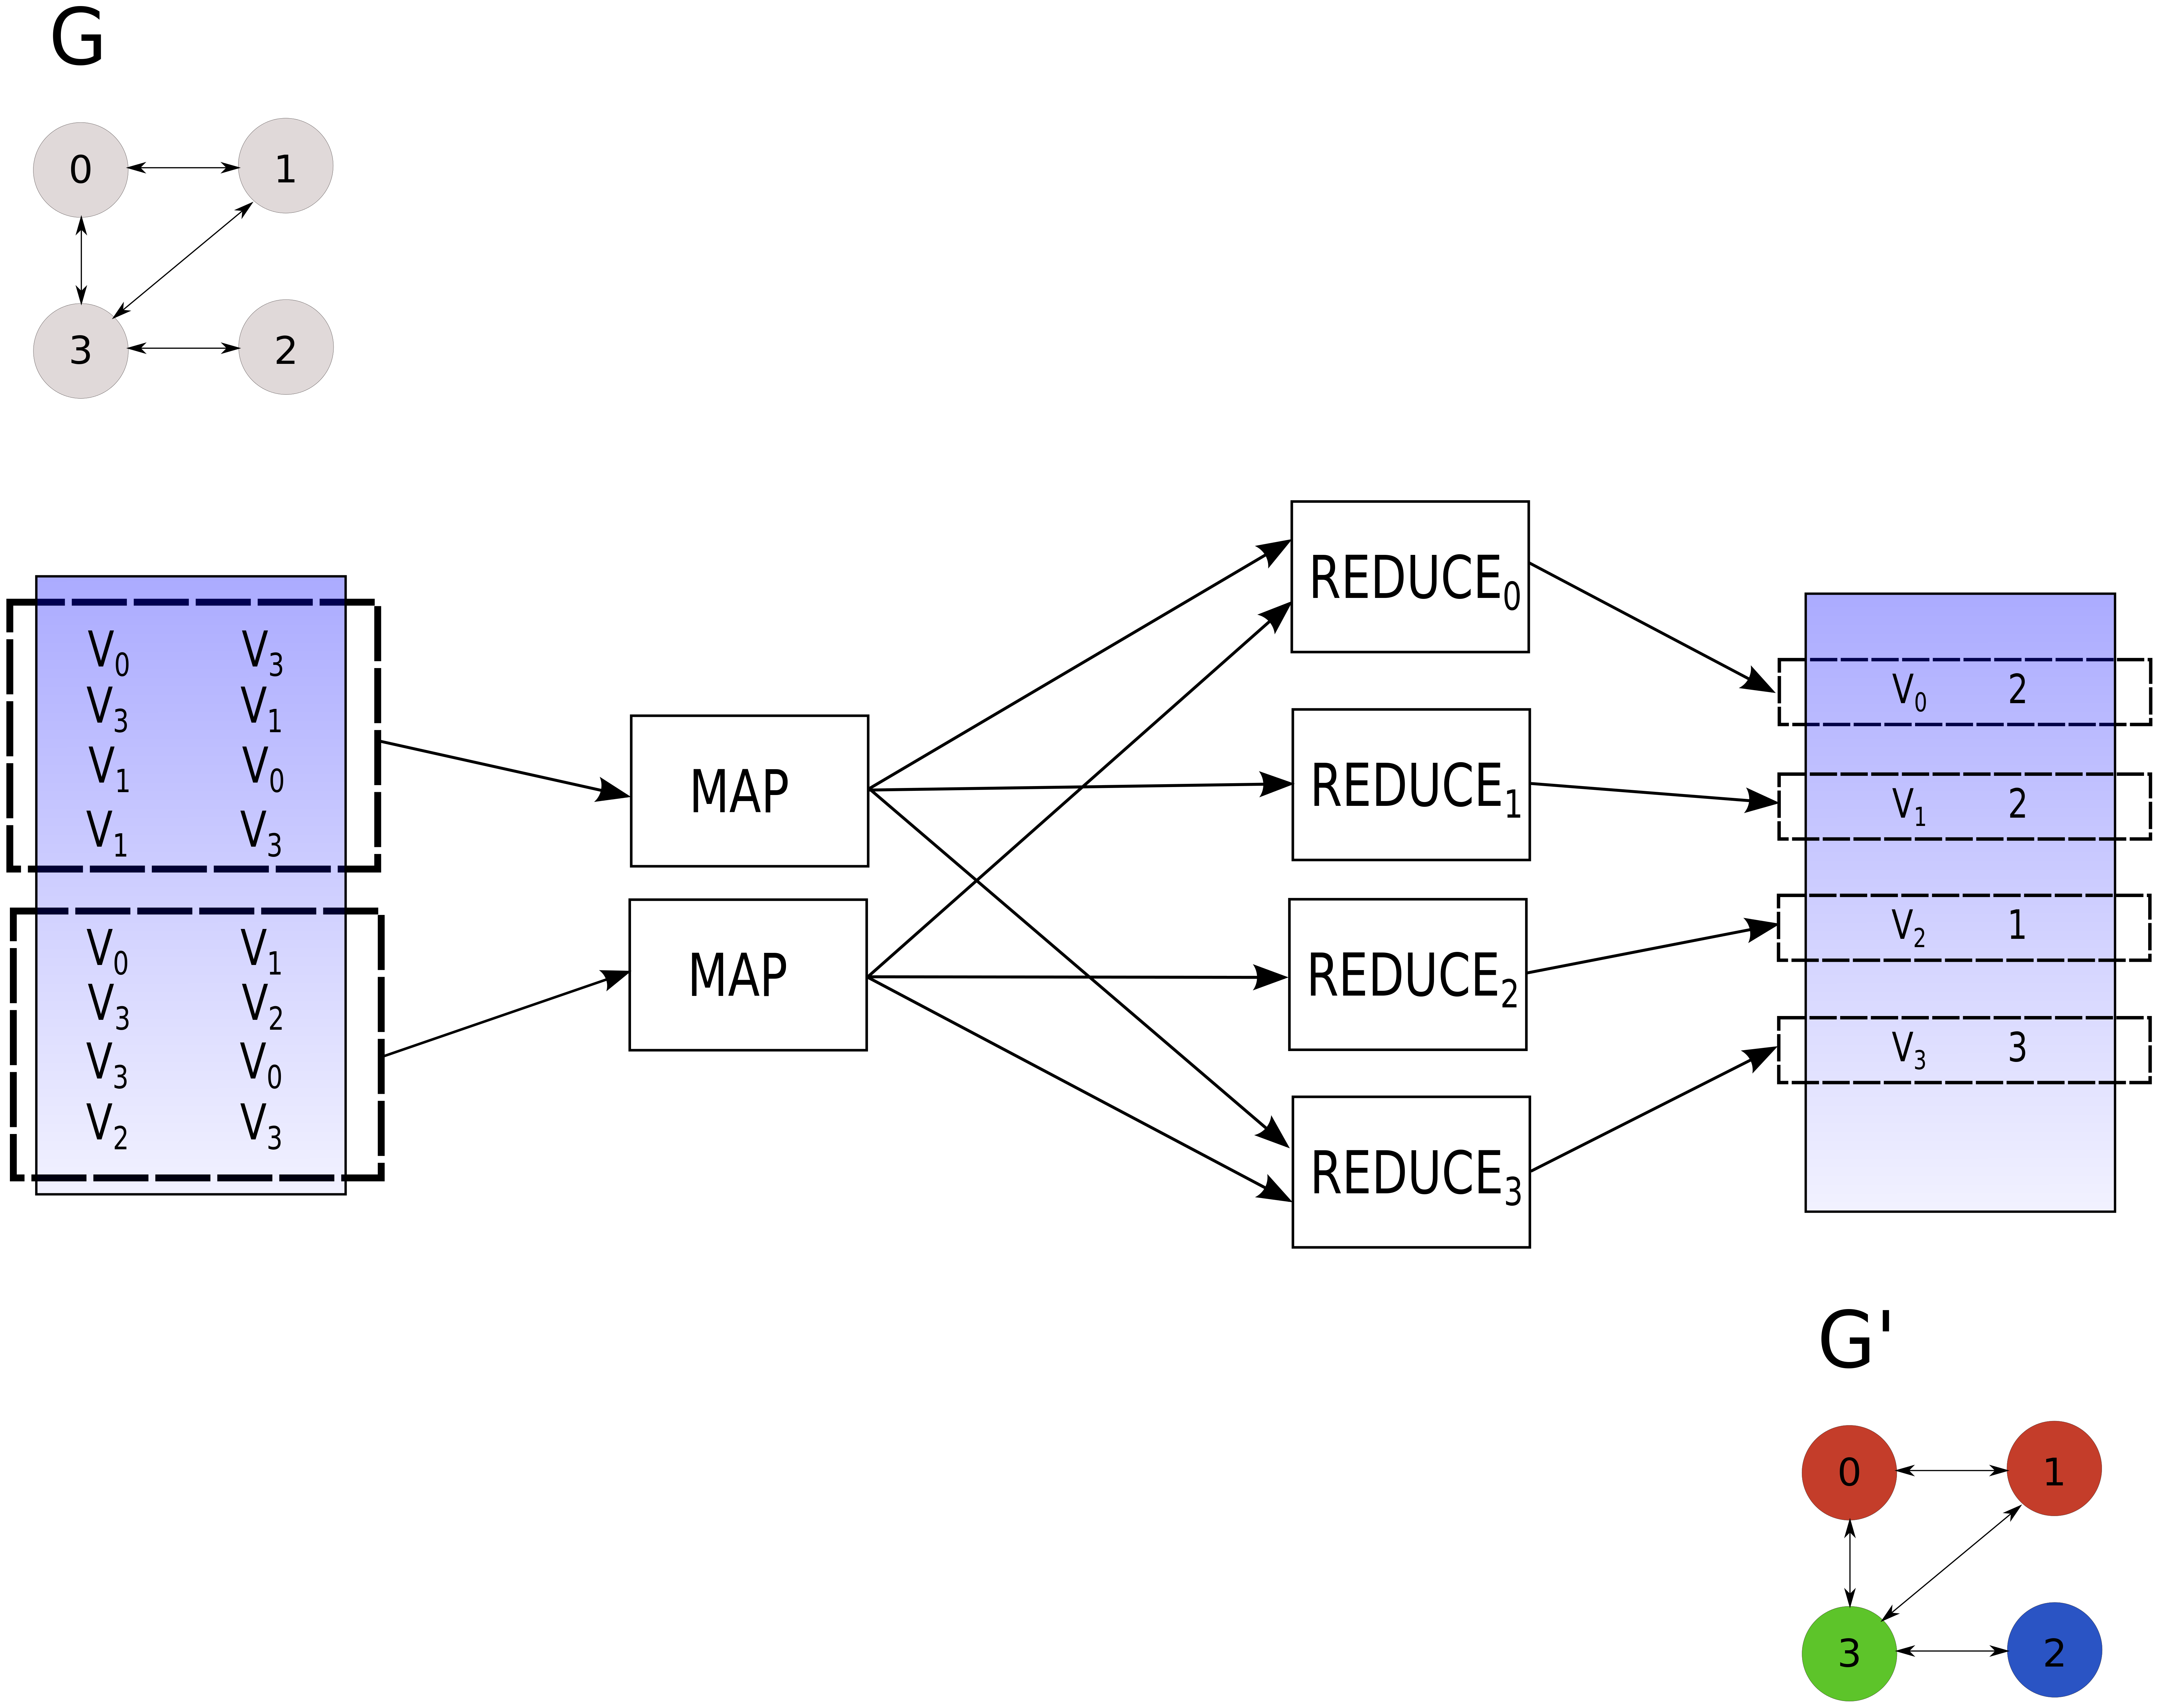
\includegraphics[width=1\textwidth]{MR-DegreeCalculator}
\caption{Esempio iterazione \textit{MapReduce DegreeCalculator}}
\label{fig:MRDEGREE}
\end{figure}

\subsection{Pregel}

L'implementazione \textit{Pregel}  di è \textit{DegreeCalculator} è composta da un solo \textit{Superstep}, rappresentata nella Figura \ref{fig:GIRAPHDEGREE}. Il valore associato ad ogni vertice né rappresenta il grado, \textit{deg(V)}).

Nel \textit{Superstep} la funzione \textit{Compute} conta gli archi associati alla struttura dati del vertice e assegna il valore calcolato a \textit{deg(V)}). Finito il primo Superstep tutti i vertici passano allo stato \textit{Vote to Halt}.

\begin{figure}
\centering
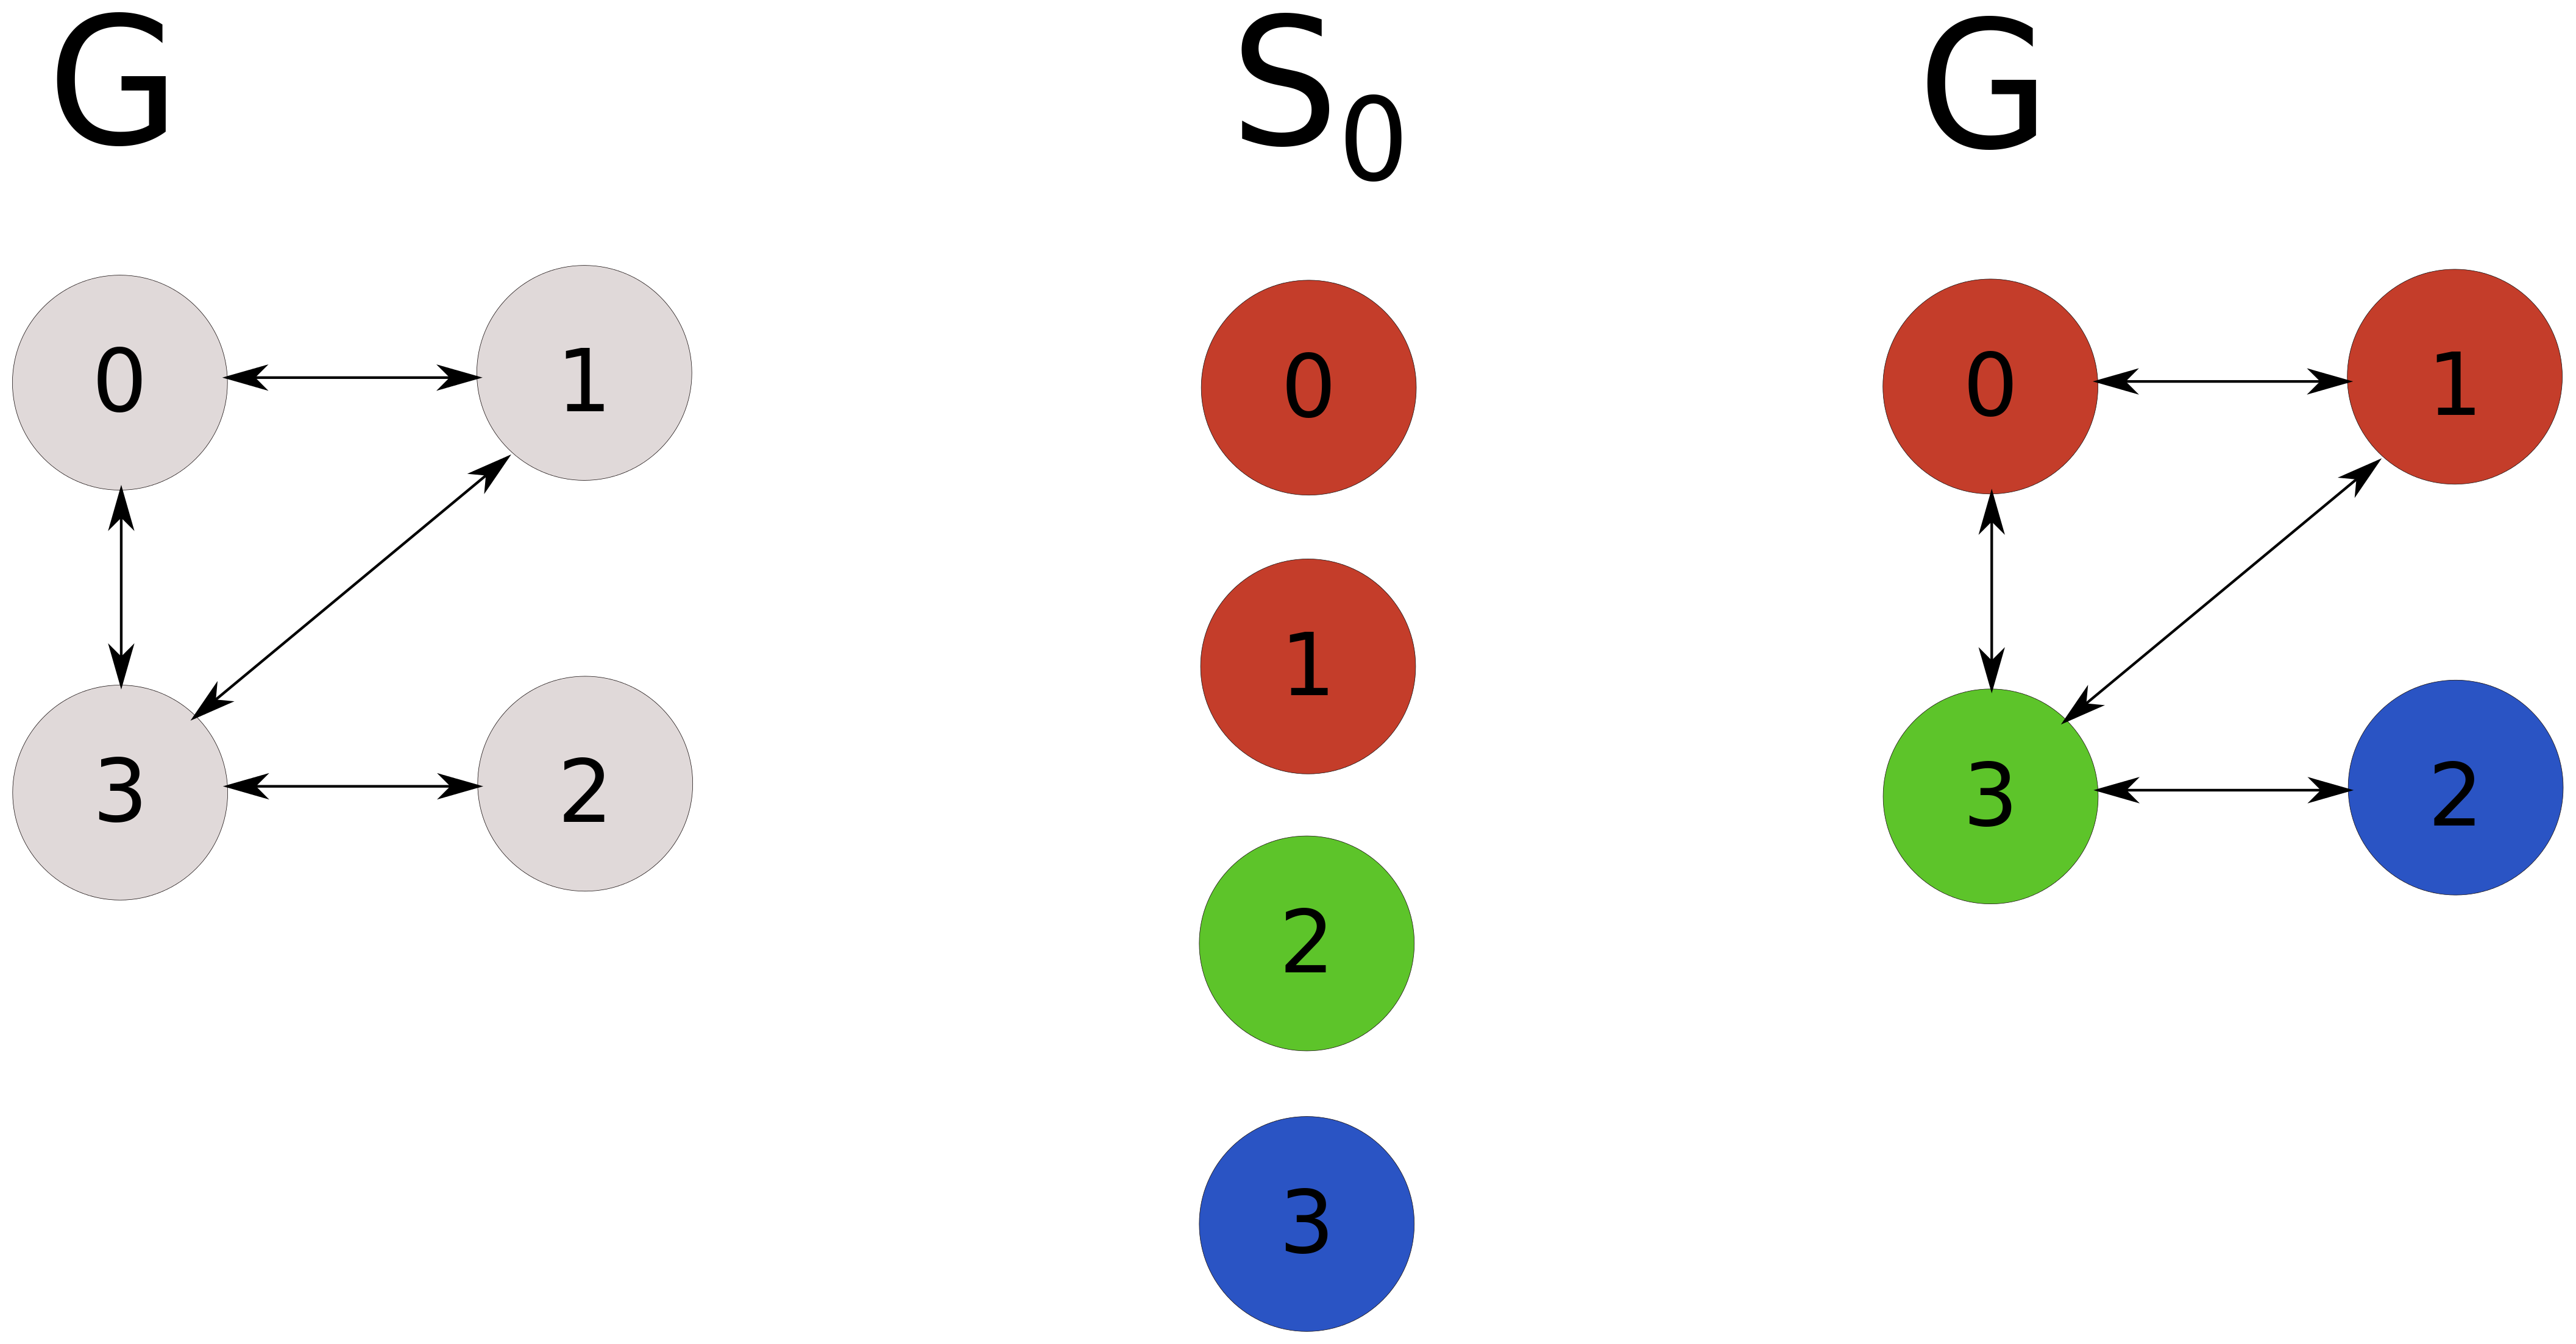
\includegraphics[width=0.8\textwidth]{Pregel-DegreeCalculator}
\caption{Esempio  \textit{Superstep} per  DegreeCalculator in \textit{Pregel}}
\label{fig:GIRAPHDEGREE}
\end{figure}

\begin{minipage}{\linewidth}[hb]
\lstinputlisting[style=customc,caption={Pseudocodice funzione \textit{Compute} in \textit{DegreeCalculator}}]{code/esempioPregele.c}
\end{minipage}

	\section{SSSP, Cammini minimi da sorgente singola}

\textit{Single Source Shortest Path (SSSP)} è l'implementazione per grafi non pesati dell'algoritmo per il calcolo di cammini minimi di Bellman-Ford. Ad ogni vertice del grafo \textit{v} è associato un valore \textit{dist\ped{v}} inizializzato a $\infty$ tranne il nodo sorgente il cui valore è inizializzato a 0.

In Figura \ref{fig:SSSP} è rappresentato un esempio di iterazione del algoritmo SSSP su di un grafo. 
Ad ogni iterazione di \textit{SSSP} ogni nodo \textit{v} confronta \textit{dist\ped{v}} con i valori \textit{dist\ped{u}} dei nodi \textit{u} adiacenti.
Il valore del nodo \textit{v} viene aggiornato nel corso dell'iterazione nel caso in cui \textit{dist\ped{v}} < \textit{min(dist\ped{u}) + 1}, con \textit{min(dist\ped{u})} valore minore tra i valori \textit{dist\ped{u}}. 

L'algoritmo termina dopo |V| iterazioni di \textit{SSSP} oppure se, nel corso di un iterazione, nessun vertice del grafo aggiorna il proprio valore \textit{dist}. 


\begin{figure}[hb]
\centering
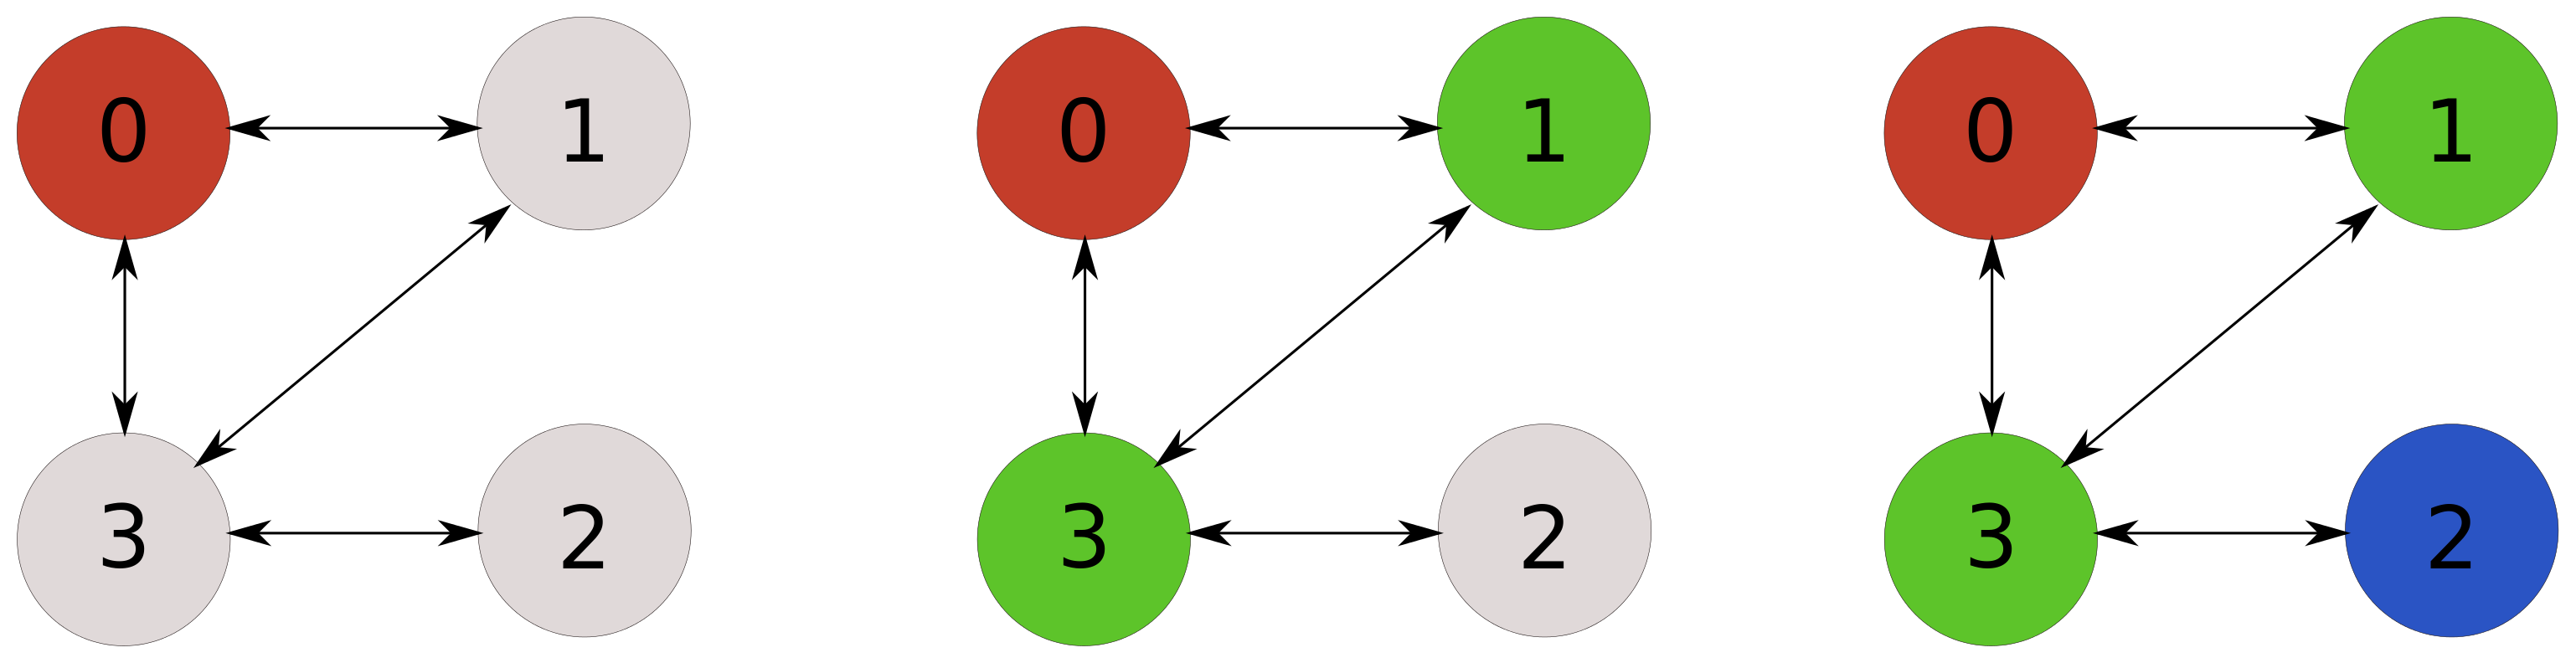
\includegraphics[width=1\textwidth]{SSSP}
\caption{Esempio iterazioni algoritmo SSSP}
\label{fig:SSSP}
\end{figure}


\subsection{MapReduce}

Per implementare SSSP nel modello \textit{MapReduce}, ogni vertice \textit{v} del grafo viene rappresentato nel formato \textit{ID\ped{v}:distanza\ped{v}}. I valori dei vertici \textit{u} del grafo  sono inizializzati a \textit{ID\ped{u}:$\infty$} tranne il nodo sorgente \textit{s} inizializzato a \textit{ID\ped{s}:0 }.

Ogni iterazione di \textit{SSSP} è implementata attraverso due iterazioni \textit{MapReduce}. L'algoritmo termina quando non vengono più modificati i valori \textit{dist} dei nodi, si esce dall'iterazione SSSP e si passa ad un ultima iterazione \textit{MapReduce} che produce in output il risultato finale dell'algoritmo. Il risultato prodotto è nel formato \textit{<ID\_nodo, dist\ped{minS}>}, dove \textit{dist\ped{minS}} è la distanza minima dal nodo sorgente.



\begin{figure}
\centering
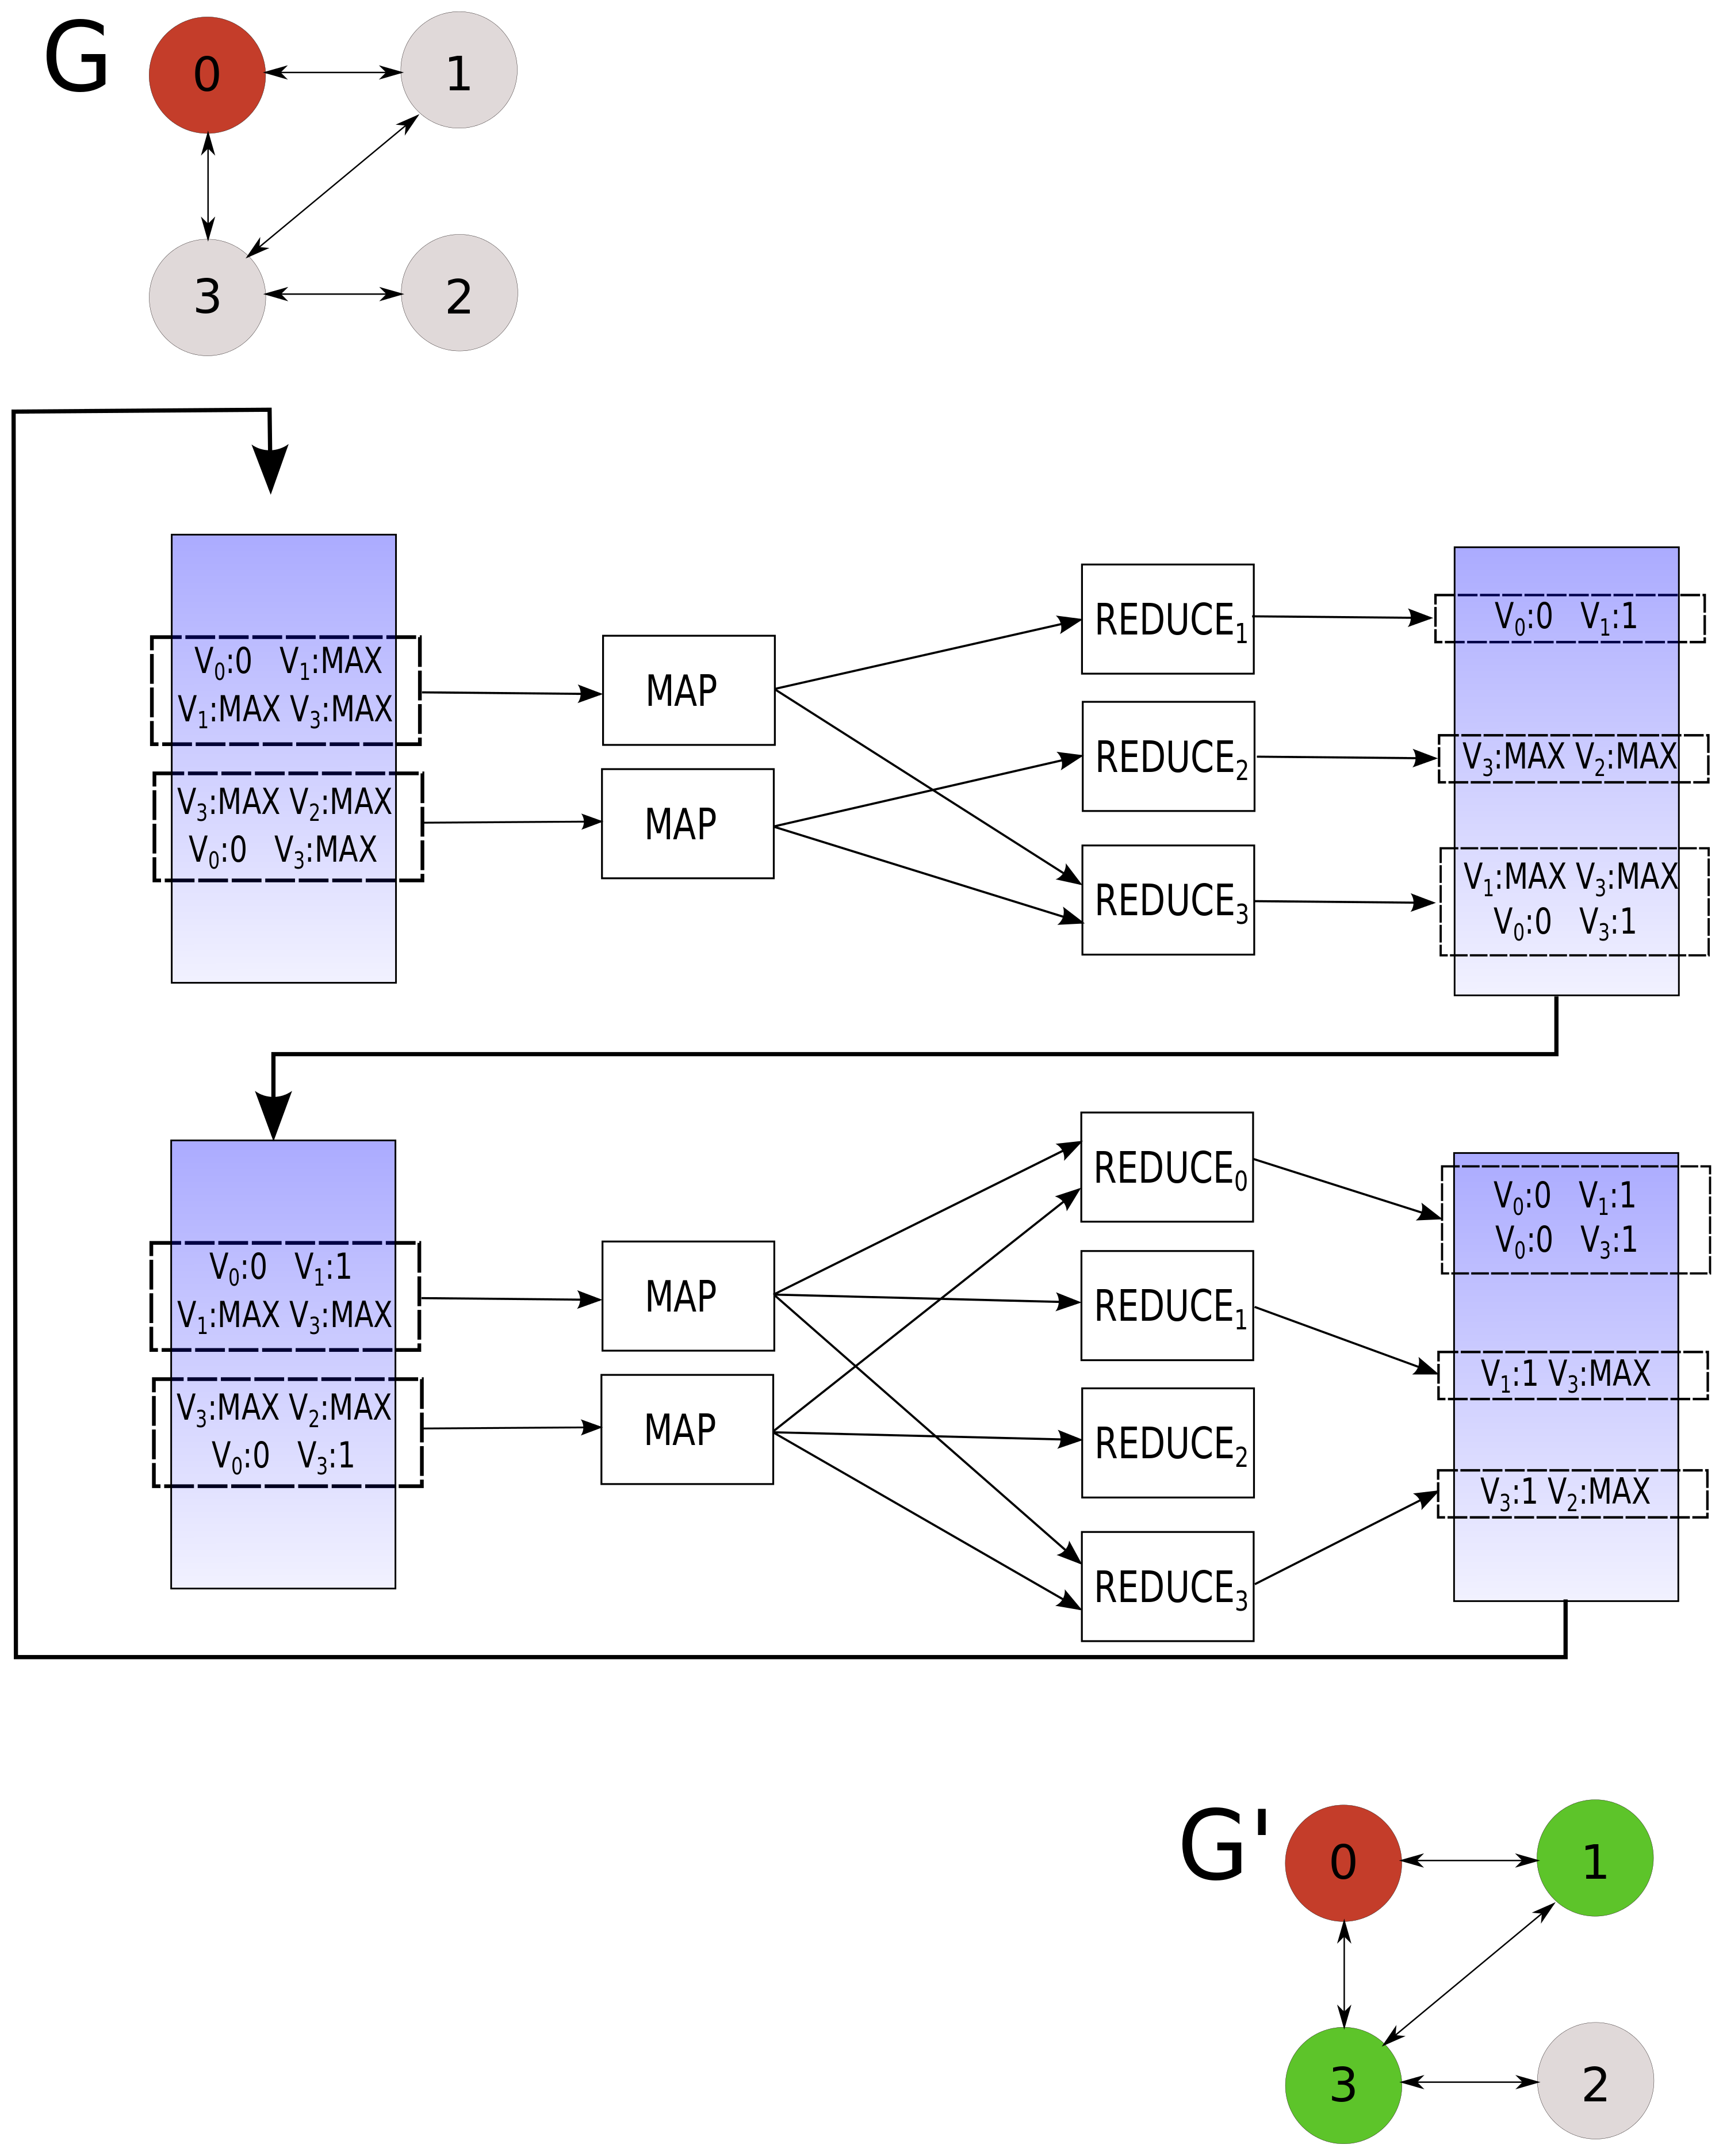
\includegraphics[width=1\textwidth]{MR-SSSP}
\caption{Esempio delle due iterazioni \textit{MapReduce} per l'esecuzione di un iterazione di \textit{SSSP}}
\label{fig:MRSSSP}
\end{figure}

In Figura \ref{fig:MRSSSP} è rappresentato un esempio di un iterazione di \textit{SSSP} in \textit{MapReduce}.
La prima iterazione \textit{MapReduce} si occupa della propagazione dei valori \textit{dist} sugli archi del grafo.
La funzione \textit{Map} è la funzione identità, prende in input la coppia di valori \textit{<v:dist\ped{v},u:dist\ped{u}>} e restituisce in output la coppia \textit{<v:dist\ped{v},u:dist\ped{u}>}.
La funzione \textit{Reduce} riceve in input la coppia di valori \textit{<v:distanza\ped{v}, list(u:distanza\ped{u})}, dove \textit{list(u:distanza\ped{u})} rappresenta la lista di nodi \textit{u} raggiungibili dal nodo \textit{v}. La funzione restituisce in output, per ogni elemento $\textit{w} \epsilon \textit{list(u:dist\ped{u})}$ la coppia di valori <v:dist\ped{v},u:dist\ped{min}>, dove il valore \textit{dist\ped{min}} è calcolato come il valore minore tra  \textit{dist\ped{i}} ed il minimo tra valori \textit{dist\ped{u} + 1} presenti in \textit{list(u:dist\ped{u})}. 

\begin{minipage}{\linewidth}
\lstinputlisting[style=customc,caption={Pseudocodice funzione \textit{Map} prima iterazione \textit{MapReduce} di \textit{SSSP}}]{code/esempioMapSSP1fase.c}		
\end{minipage}

\begin{minipage}{\linewidth}
\lstinputlisting[style=customc,caption={Pseudocodice funzione \textit{Reduce}prima iterazione \textit{MapReduce} di \textit{SSSP}} ]{code/esempioReduceSSP1fase.c}		
\end{minipage}

La seconda iterazione \textit{MapReduce} si occupa di aggiornare i valori \textit{dist} relativi ai  nodi sorgenti degli archi, in quanto dopo la prima iterazione sono aggiornati soltanto i nodi destinazione. 

La funzione \textit{Map} della seconda  iterazione prende in input gli archi nel formato \textit{<v:dist\ped{v},u:dist\ped{u}>} e produce il doppio output formato dalle coppie \textit{<v, u:dist\ped{u}:dist\ped{v}:S>} e \textit{<u ,v:dist\ped{v}:dist\ped{u}:D>}, \textit{S} e \textit{D} sono dei valori segnaposto predefiniti, \textit{S} serve a segnalare che il nodo v è il nodo di partenza dell'arco e \textit{D} che è il nodo destinazione. I valori sentinella vengono utilizzati nella funzione \textit{Reduce} per garantire che gli archi vengano ricostruiti con la direzione corretta.

La funzione \textit{Reduce} della seconda fase prende in input la coppia di valori \textit{<v, list(u:distanza\ped{u}:distanza\ped{v}:\$)} con \textit{$\$ \epsilon [S,D]$}. 
Per ogni valore presente nella lista  \textit{<v, list(u:distanza\ped{u}:distanza\ped{v}:\$)} con \$ = \textit{S}, la funzione \textit{Reduce} produce in output la coppia di valori \textit{<v:dist\_min\ped{i}: u:dist\ped{u}>}, dove \textit{dist\_min\ped{i}} è il minore dei valori \textit{dist\ped{i}} in \textit{list(v\ped{j}:dist\ped{j}:dist\ped{i}:\$) con \$ = \textit{D}}.

Le iterazioni \textit{SSSP} terminano quando non si verificano aggiornamenti di valori \textit{dist} durante la  prima iterazione \textit{MapReduce}.

\begin{minipage}{\linewidth}
\lstinputlisting[style=customc,caption={Pseudocodice funzione \textit{Map} SSSP}]{code/esempioMapSSP2fase.c}		
\end{minipage}

\begin{minipage}{\linewidth}
\lstinputlisting[style=customc,caption={Pseudocodice funzione \textit{Reduce} SSSP}]{code/esempioReduceSSP2fase.c}		
\end{minipage}

L'ultima iterazione \textit{MapReduce}, in cui vengono salvati i risultati prodotti, viene eseguita a l termine  delle iterazioni \textit{SSSP}.
La funzione \textit{Map} prende in input la coppia di valori \textit{<v:dist\ped{v}, u:dist\ped{u}>}  e produce in output la coppia \textit{<v:dist\ped{v}, $\varepsilon$>}, dove $\varepsilon$ è la stringa vuota.

La funzione \textit{Reduce} prende in input la coppia di valori \textit{<v:dist\ped{v},list($\varepsilon$)>} e produce in output la coppia \textit{<v, dist\ped{v}>} con \textit{dist\ped{v}} valore del cammino minimo dal nodo sorgente al nodo \textit{v}.


\begin{minipage}{\linewidth}
\lstinputlisting[style=customc,caption={Pseudocodice funzione \textit{Map} SSSP}]{code/esempioMapSSP3fase.c}		
\end{minipage}
\begin{minipage}{\linewidth}
\lstinputlisting[style=customc,caption={Pseudocodice funzione \textit{Reduce} SSSP}]{code/esempioReduceSSP3fase.c}
\end{minipage}		

\subsection{Pregel}

L'implementazione in \textit{Pregel} per l'algoritmo \textit{SSSP}, rappresentata in Figura \ref{fig:PREGELSSSP}, è costituita da un primo \textit{Superstep} dove il valore associato al vertex \textit{v},  che rappresenta il valore \textit{dist\ped{v}} associato a \textit{v}, viene inizializzato a $\infty$ tranne per il vertice sorgente il cui valore è inizializzato a 0.


Ad ogni \textit{Superstep S} è eseguita un'iterazione \textit{SSSP} in cui un vertice \textit{v} riceve i messaggi, inviati durante il \textit{Superstep S-1}, messaggi che contengono il valore \textit{distanza\ped{u}} dei vertici \textit{u} a cui \textit{v} è adiacente.
Il vertice \textit{v} confronta i messaggi ricevuti con il proprio valore \textit{dist\ped{v}}. Nel caso che almeno uno dei messaggi contiene un valore \textit{dist\ped{u}} minore, il valore di \textit{dist\ped{v}} viene aggiornato con il minore tra i valori contenuti nei messaggi.
Nel caso il vertice \textit{v} viene aggiornati nel \textit{Superstep S}, nel corso della stessa iterazione, viene inviato un messaggio contenente il nuovo valore \textit{dist\ped{v} + 1} ai vertici vicini di \textit{v}, che verrà ricevuto nel \textit{Superstep S+1}. Tutti i vertici passano allo stato \textit{Vote to Halt} e solo i vertici a cui è stato inviato un messaggio in S+1 passeranno nuovamente ad uno stato \textit{Active} nel  \textit{Superstep S+1}.
La computazione di \textit{SSSP} termina quando nessun vertice invia messaggi nel corso del \textit{Superstep} e quindi nessuno dei vertici del grafo ha aggiornato il valore \textit{distanza}.

In \ref{lst:psudoSSSPGiraph} è mostrato lo pseudocodice della funzione \textit{compute} per il calcolo in Pregel di SSSP.



\begin{figure}
\centering
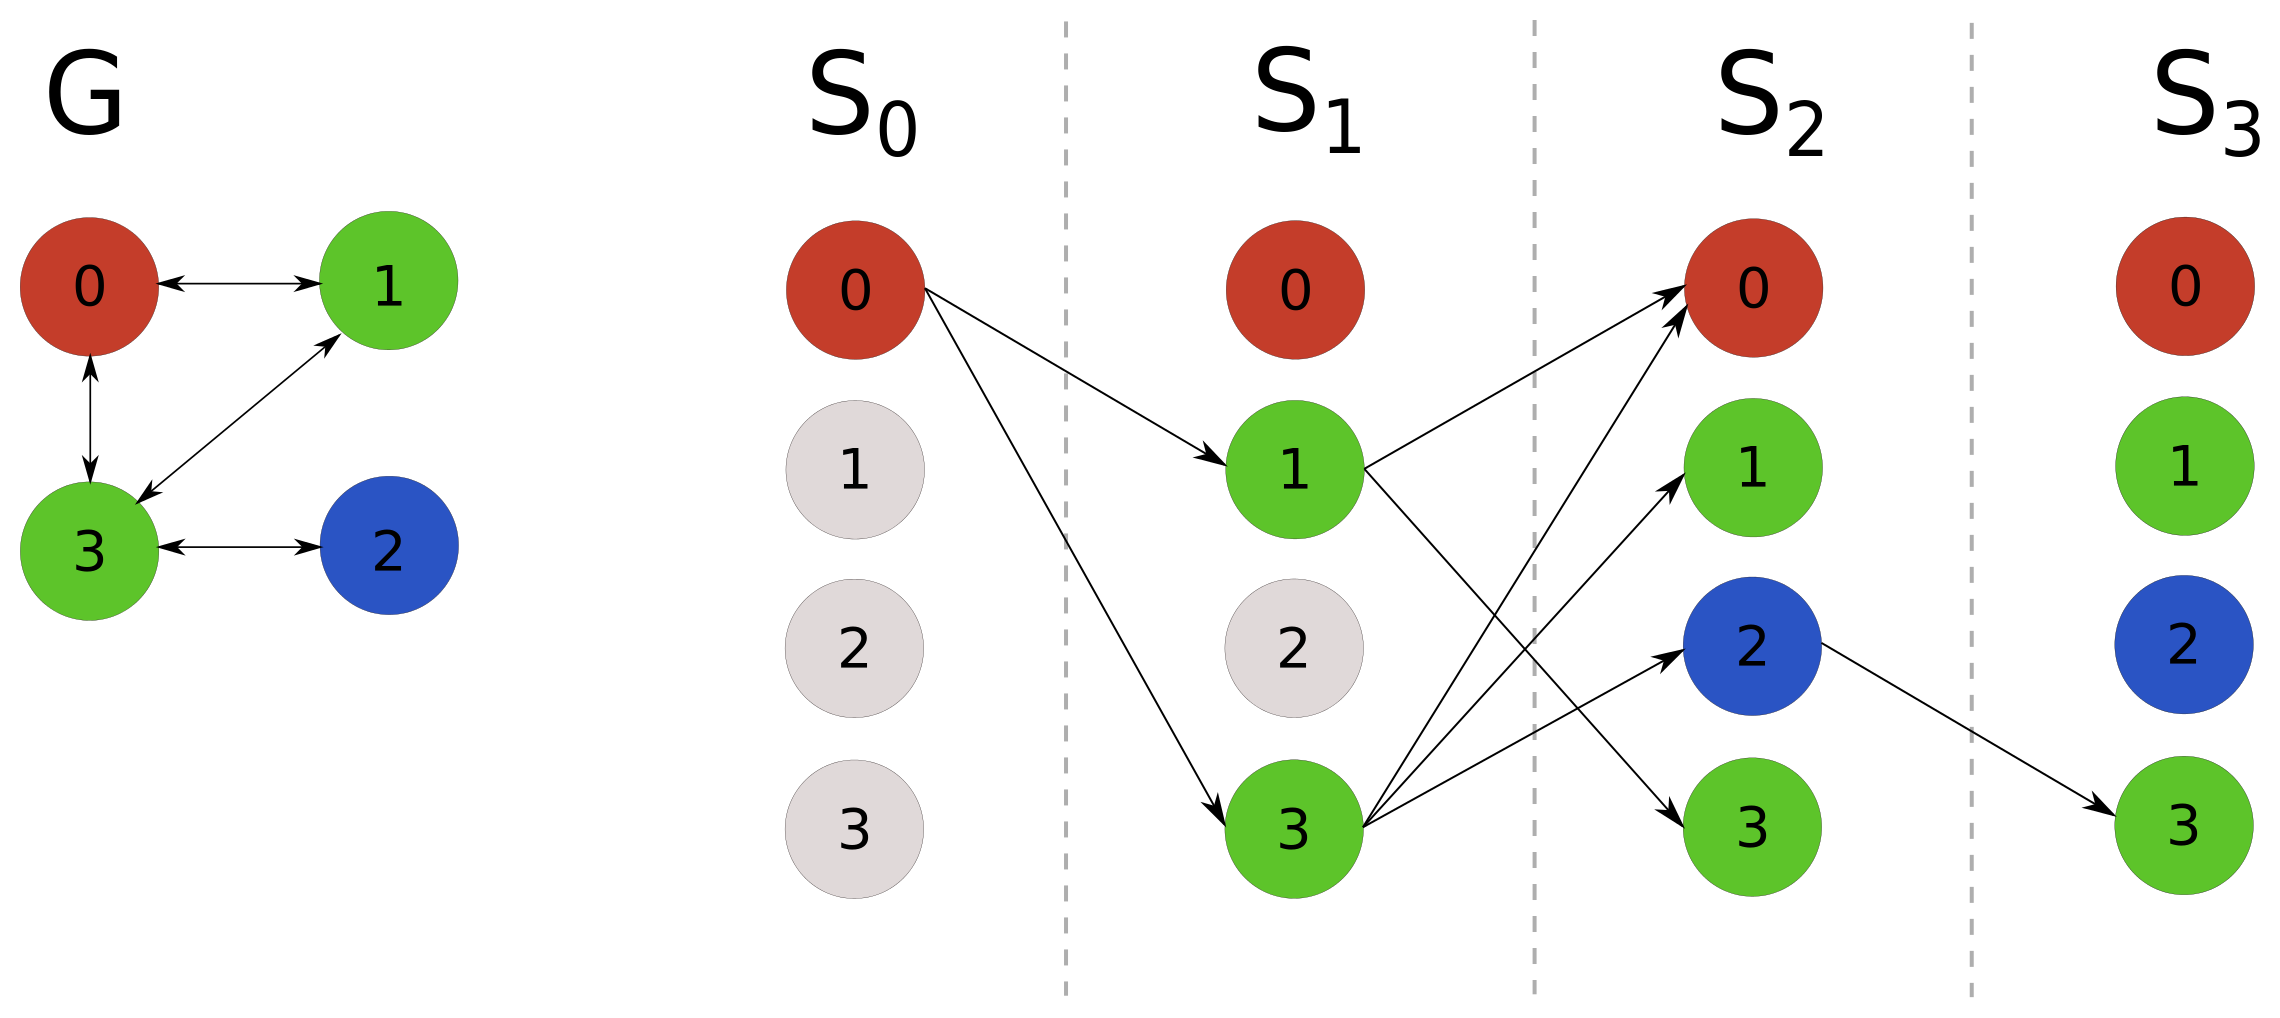
\includegraphics[width=1\textwidth]{PREGEL-SSSP}
\caption{Esempio SSSP in Pregel}
\label{fig:PREGELSSSP}
\end{figure}


\begin{minipage}{\linewidth}
\lstinputlisting[style=customc,caption={Pseudocodice funzione \textit{Compute} SSSP},label={lst:psudoSSSPGiraph}	]{code/esempioPregeleSSSP2.c}	
\end{minipage}


\section{NodeIterator++, Calcolo del numero di triangoli del grafo}

NodeIterator++ \cite{Suri:2011:CTC:1963405.1963491} è un algoritmo per il calcolo del numero di triangoli in un grafo in modo efficiente nel modello MapReduce \cite{Dean:2008:MSD:1327452.1327492}.
L'idea di base dell'algoritmo è di costruire, per ogni nodo \textit{v} del grafo, una lista di tutte le possibili coppie \textit{(u,w)} di nodi adiacenti a \textit{v}. Per ogni coppia di nodi \textit{(u,w)}, se \textit{(u,w)$\in$ E}, con \textit{E} insieme degli archi del grafo, allora i nodi \textit{ v, u e w } formano un triangolo del grafo.
 
Nella versione base dell'algoritmo, \textit{NodeIterator}, vengono prese in esame tutte le coppie possibili di nodi vicine di un nodo \textit{v}, questo portava a contare ogni triangolo sei volte in quanto, per ogni nodo appartenente ad un triangolo, esistono due coppie di nodi vicini appartenenti all'insieme di archi del grafo.

Per migliorare l'efficienza di \textit{NodeIterator} contando ogni triangolo una volta, nella versione \textit{NodeIterator++} dell'algoritmo, viene utilizzato una relazione di ordine totale sui vertici del grafo, \textit{prec} ($\prec$). Per una coppia di nodi del grafo \textit{u} e \textit{w} del grafo, si ha che \textit{u $\prec$ w} se \textit{deg(u) < deg(w)}, dove \textit{deg(v)} è il grado del nodo \textit{v}. In caso di nodi con lo stesso grado si sceglie in modo arbitrario e consistente l'ordine di precedenza tra i nodi, come per esempio l'ordine sul valore numerico corrispondente all'identificativo del nodo. Lo pseudocodice  relativo a \textit{NodeIterator++} è mostrato in \ref{lst:pseudoNodepp}.

\begin{minipage}{\linewidth}
\lstinputlisting[style=customc,caption={Pseudocodice algortimo NodeIterator++},label={lst:pseudoNodepp}]{code/nodeiterator.c}	
\end{minipage}


\subsection{MapReduce}

Per testare l'algoritmo \textit{NodeIterator++} in \textit{MapReduce} ho utilizzato l'implementazione realizzata da Irene Finocchi, Marco Finocchi, Emanuele G. Fusco in \cite{DBLP:journals/corr/FinocchiFF14}.

Per implementare \textit{NodeIterator++ } sono necessari due iterazione \textit{MapReduce}. Nella prima iterazione vengono generate tutte le coppie di vicini di un nodo \textit{v}, \textit{(u,v)}.

La funzione \textit{Map}, il cui pseudocodice è mostrato in \ref{lst:nodeiteratorMRMapfase1}, riceve in input un arco del grado nella forma \textit{<v, u>} e produce in output la coppia di vertici \textit{<v, u>} soltanto se \textit{v $\prec$ u}.

La funzione \textit{Reduce} riceve in input la coppia \textit{<v,list(u)>}, con \textit{list(u)} lista di nodi vicini di \textit{v} per cui \textit{v $\prec$ u}. Per ogni coppia di elementi  di \textit{list(u)}, \textit{(u,w)} produce in output la coppia di valori \textit{<v, (u,w)>}. Lo pseudocodice della funzione \textit{Reduce} è mostrato in \ref{lst:nodeiteratorMRReducefase1}.

\begin{minipage}{\linewidth}	
\lstinputlisting[style=customc,caption={Pseudocodice Map Fase 1 NodeIterator++},label={lst:nodeiteratorMRMapfase1}]{code/nodeiteratorMRMapfase1.c}	
\end{minipage}

\begin{minipage}{\linewidth}
\lstinputlisting[style=customc,caption={Pseudocodice Reduce Fase 1  NodeIterator++},label={lst:nodeiteratorMRReducefase1}]{code/nodeiteratorMRReducefase1.c}	
\end{minipage}

Nella seconda fase MapReduce vengono verificate quali tra le coppie di nodi, generate dalla prima iterazione \textit{MapReduce}, hanno un arco che collega i due vertici e che quindi costituiscono un triangolo del grafo. 

La funzione \textit{Map} prende in input i valori da due differenti sorgenti: l'output del round precedente, \textit{<v,(u,w)>} e la lista di archi \textit{<v,u>} dall'input iniziale del iterazione \textit{SSSP}. Per il primo tipo di input è prodotto in output la coppia di valori \textit{<(u,w),v>}, per il secondo tipo di input, invece, è prodotto in output la coppia di valori \textit{<(v,u), \$>}, dove \$ è un simbolo segnaposto. Il simbolo \$ è utilizzato poi nella funzione di \textit{Reduce} come simbolo che segnala che la coppia di nodi \textit{(v,u)} è collegata da un arco del grafo.

La funzione \textit{Reduce} prende in input la coppia \textit{<(u,v), list(w)>}, dove \textit{(u,v)} è un arco del grafo e \textit{list(w)} è una lista di elementi \textit{w}, dove  l'elemento \textit{w} o è un vertice del grafo o è il valore segnaposto \$.
Se nella lista \textit{list(w)} è presente il valore \$ allora l'arco \textit{$(u,v) \in E$}, con \textit{E} insieme degli archi del grafo. In questo caso ogni valore elemento \textit{list(w)}, \textit{w} diverso da \$, rappresenta un nodo del grafo che ha come vicino sia il nodo \textit{u} che il nodo \textit{w}, per cui la presenza dell'arco \textit{(u,v)} "chiude" il triangolo \textit{(u,v,w)}. 
L'output della funzione \textit{Reduce}, nel caso \textit{$\$\in list(w)$}, è la coppia di valori \textit{<(u,v), T>}, dove \textit{T} è il numero di triangoli "chiusi" dalla coppia \textit{(u,v)}. Nel caso in cui \textit{$\$\notin list(w)$} allora la coppia \textit{(u,v)} non ha un arco che collega i 2 vertici, nessuno dei possibili triangolo segnalati in list(w) è "chiuso" e la funzione non produce nessun valore in output.
In \ref{nodeiteratorMRReducefase2} e  \ref{nodeiteratorMRReducefase2} sono mostrati, rispettivamente, lo pseudocodice della funzione \textit{Map} e della funzione \textit{Reduce}.

In Figura \ref{fig:MRNIT} è rappresentato un esempio della computazione di \textit{NodeIterator++} in \textit{Mapreduce}.

Per ricavare il numero totale di triangoli è necessario un iterazione aggiuntiva, implementabile sempre in \textit{MapReduce}, in cui vengono contate le somme parziali dei triangoli ricavate  nell'iterazione precedente. La funzione \textit{Map} mappa l'output dell'iterazione precedente, formato dalle coppie \textit{<(u,v), T>}, verso un unica funzione \textit{Reduce} utilizzando un unica chiave. La funzione \textit{Reduce} riceve tutti i risultati parziali \textit{T} ricavati nel passo precedente, li somma tra loro e fornisce in output il risultato totale dei triangoli presenti nel grafo.


\begin{minipage}{\linewidth}
\lstinputlisting[style=customc,caption={Pseudocodice Map Fase 2 NodeIterator++},label={lst:nodeiteratorMRMapfase2}]{code/nodeiteratorMRMapfase2.c}	
\end{minipage}
\begin{minipage}{\linewidth}
\lstinputlisting[style=customc,caption={Pseudocodice Reduce Fase 2  NodeIterator++},label={lst:nodeiteratorMRReducefase2}]{code/nodeiteratorMRReducefase2.c}	
\end{minipage}


\begin{figure}
\centering
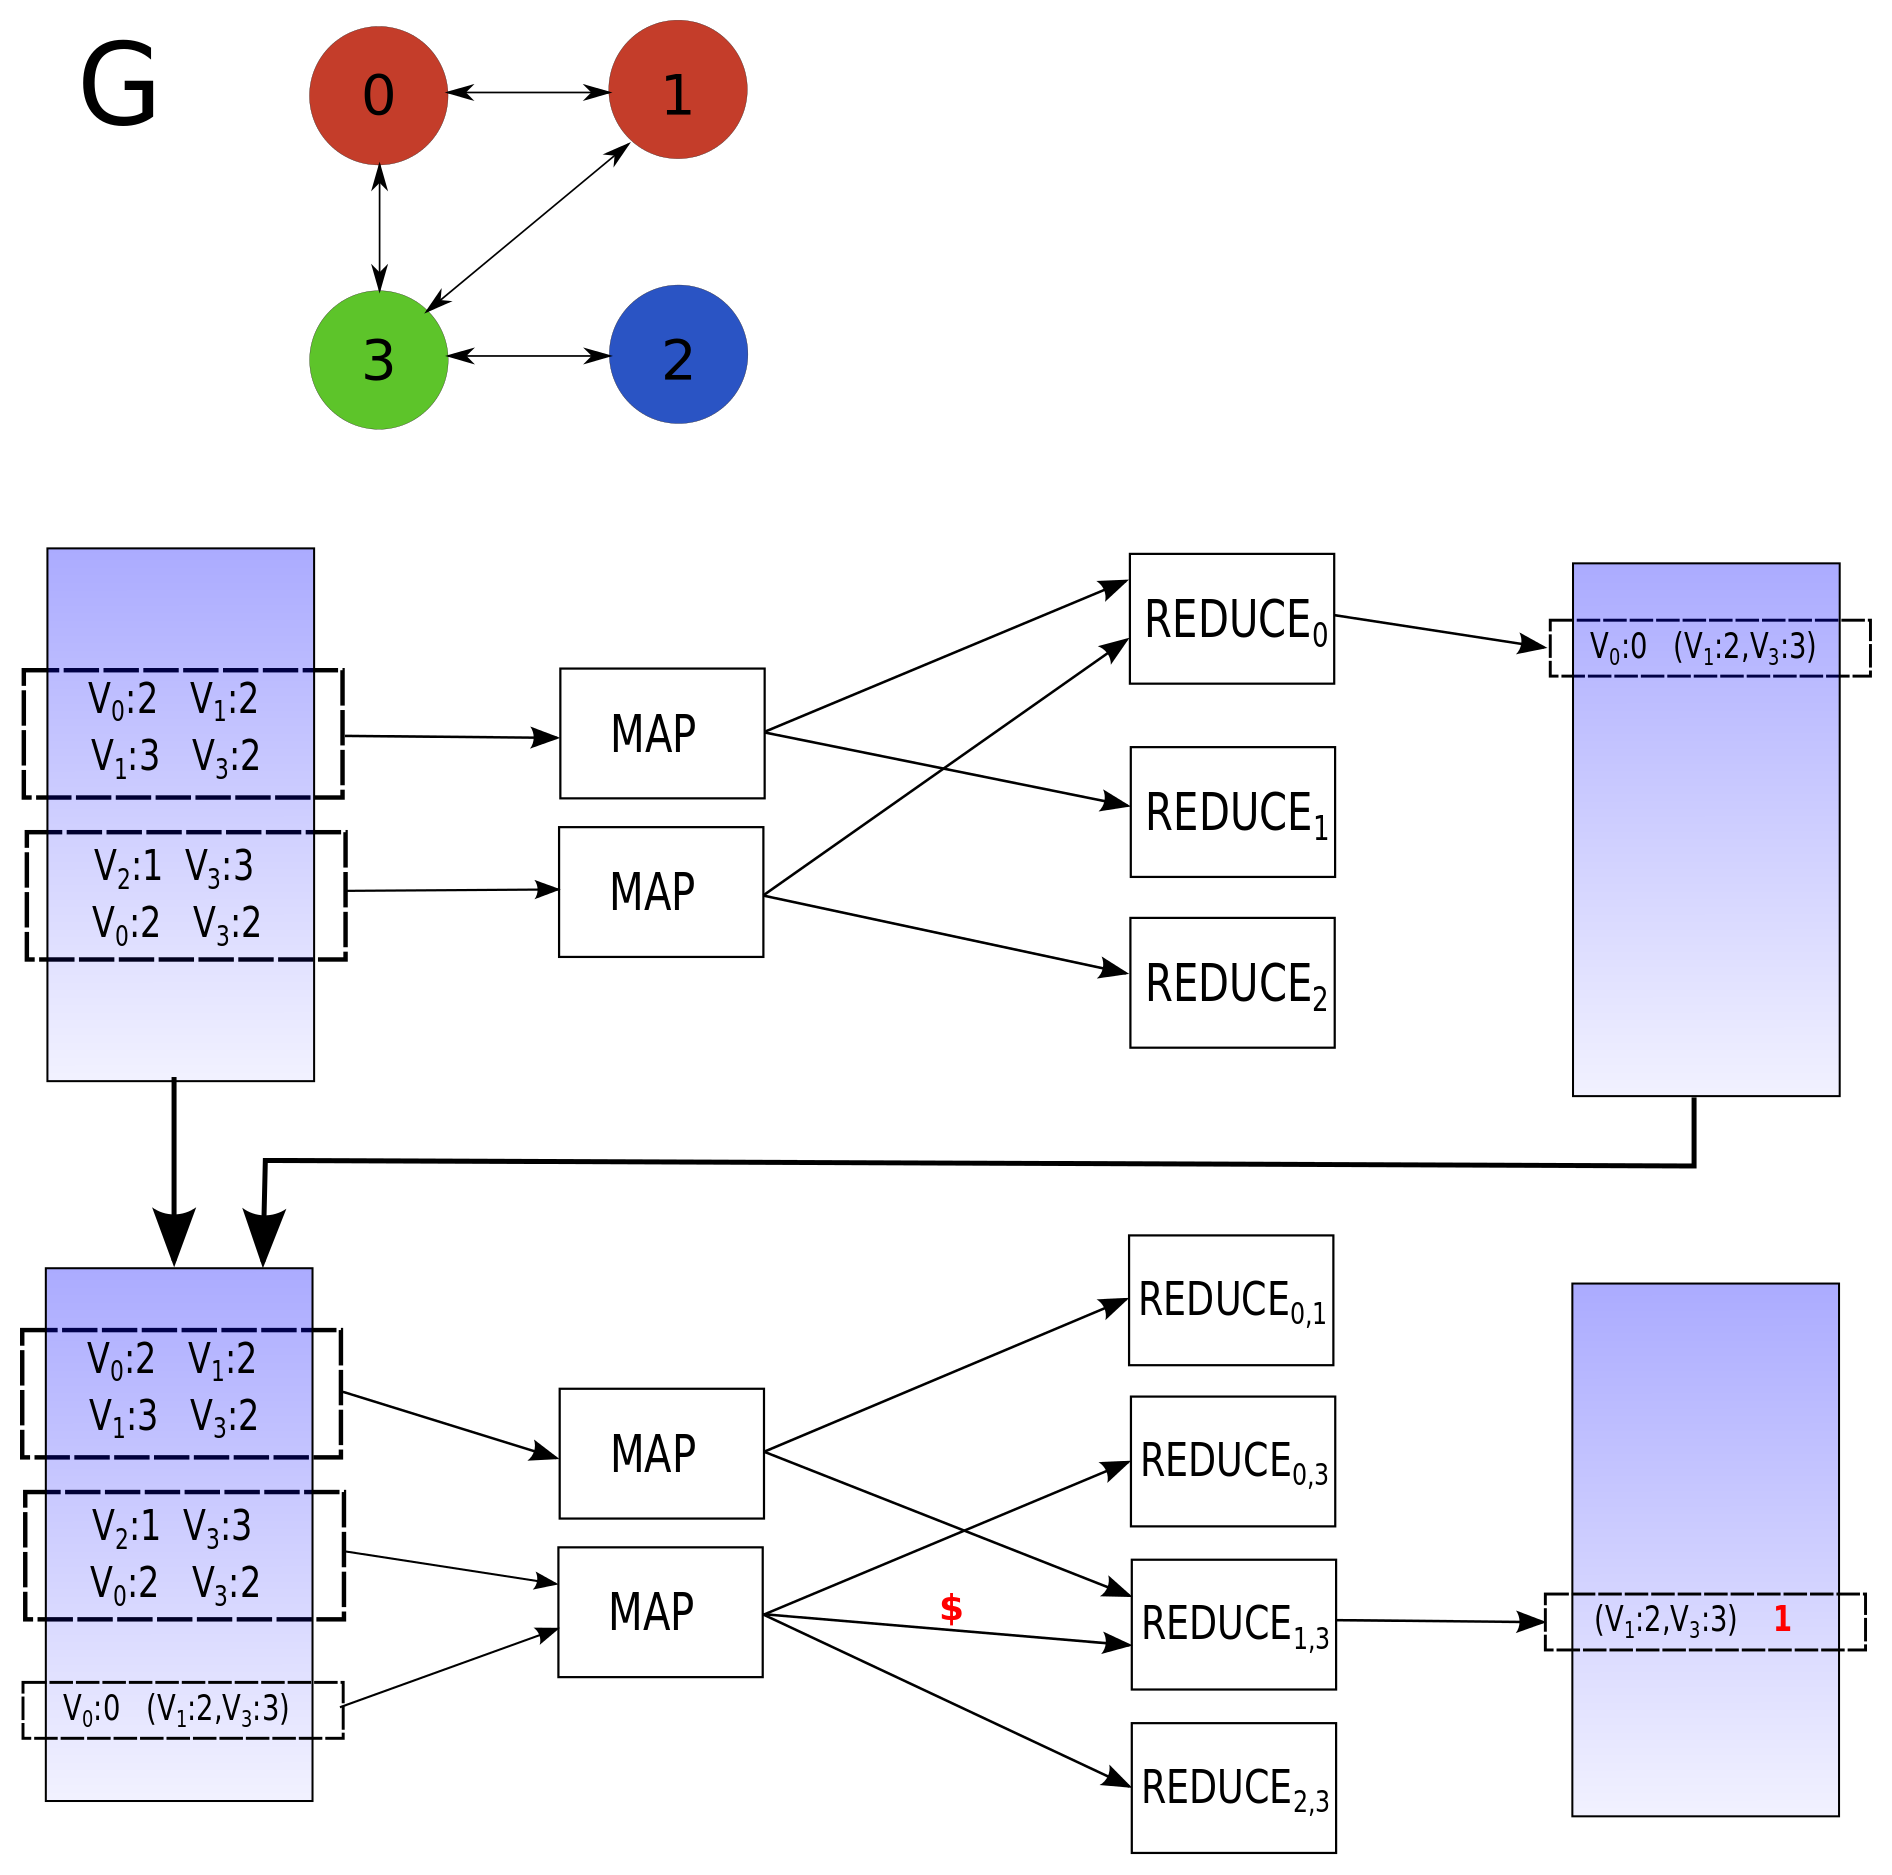
\includegraphics[width=1\textwidth]{MR-trianglepp}
\caption{Esempio calcolo \textit{NodeIterator++} in \textit{MapReduce}}
\label{fig:MRNIT}
\end{figure}

\subsection{Pregel}

L'implementazione realizzata per \textit{NodeIterator++} su \textit{Pregel}, il cui pseudocodice è riportato in \ref{lst:esempioPregeleNodeIterator}, prevede l'esecuzione di quattro \textit{Superstep} :

\begin{enumerate}
\item Nel primo \textit{Superstep} il vertice \textit{v} calcola ed invia a tutti i nodi vicini il valore \textit{deg(v)}, grado di \textit{v}. 

\item Nel secondo \textit{Superstep} il vertice \textit{v} confronta il proprio grado con il grado dei nodi ricevuti attraverso la funzione di ordine totale $\prec$ definita in \textit{NodeIterator++}. 
Per ogni coppi di archi orientati, che compongono l'arco non orientato in \textit{Pregel}, viene eliminato l'arco con il verso che non rispetta l'ordine $\prec$.
Come nell'esempio in \ref{fig:PREGELNIT}, nel grafo \textit{G'}, dopo il secondo \textit{Superstep S\ped{1}}, rimangono solo gli archi che rispettano l'ordine definito da $\prec$, in questo caso gli archi \textit{(0,1)}, \textit{(0,3)}, \textit{(1,3)} e \textit{(2,3)}.

\item Nel terzo \textit{Superstep}, il vertice \textit{v} invia a tutti i nodi, collegati a \textit{v} da un arco del grafo ottenuto dopo l'iterazione precedente, la lista dei nodi vicini.

\item Nel ultimo \textit{Superstep}, il vertice \textit{v} riceve tramite messaggi la lista dei nodi dai vertici \textit{w} a cui è vicino, \textit{list(w)}. Nel caso in cui l'arco \textit{(v,u)} è un arco del grafo, con \textit{$u \in list(w)$}, allora i nodi \textit{(u, v, w)} formano un triangolo nel grafo. 
Il vertice \textit{v} confronta, quindi, la lista dei nodi ricevuta con l'insieme di vertici raggiungibili da \textit{v}. 
Per ogni corrispondenza segnala il triangolo individuato tramite l'utilizza di un aggregatore di tipo \textit{SUM}, visto nel capitolo introduttivo su \textit{Pregel}.
\end{enumerate}

Alla fine del \textit{Superstep}, attraverso il meccanismo degli aggregatori, il nodo Master raccoglie tutti i valori aggregati ottenendo il numero totale di triangoli presenti nel grafo.

\lstinputlisting[style=customc,caption={Pseudocodice NodeIterator++ Pregel},label={lst:esempioPregeleNodeIterator}]{code/esempioPregeleNodeIterator.c}	

\begin{figure}
\centering
 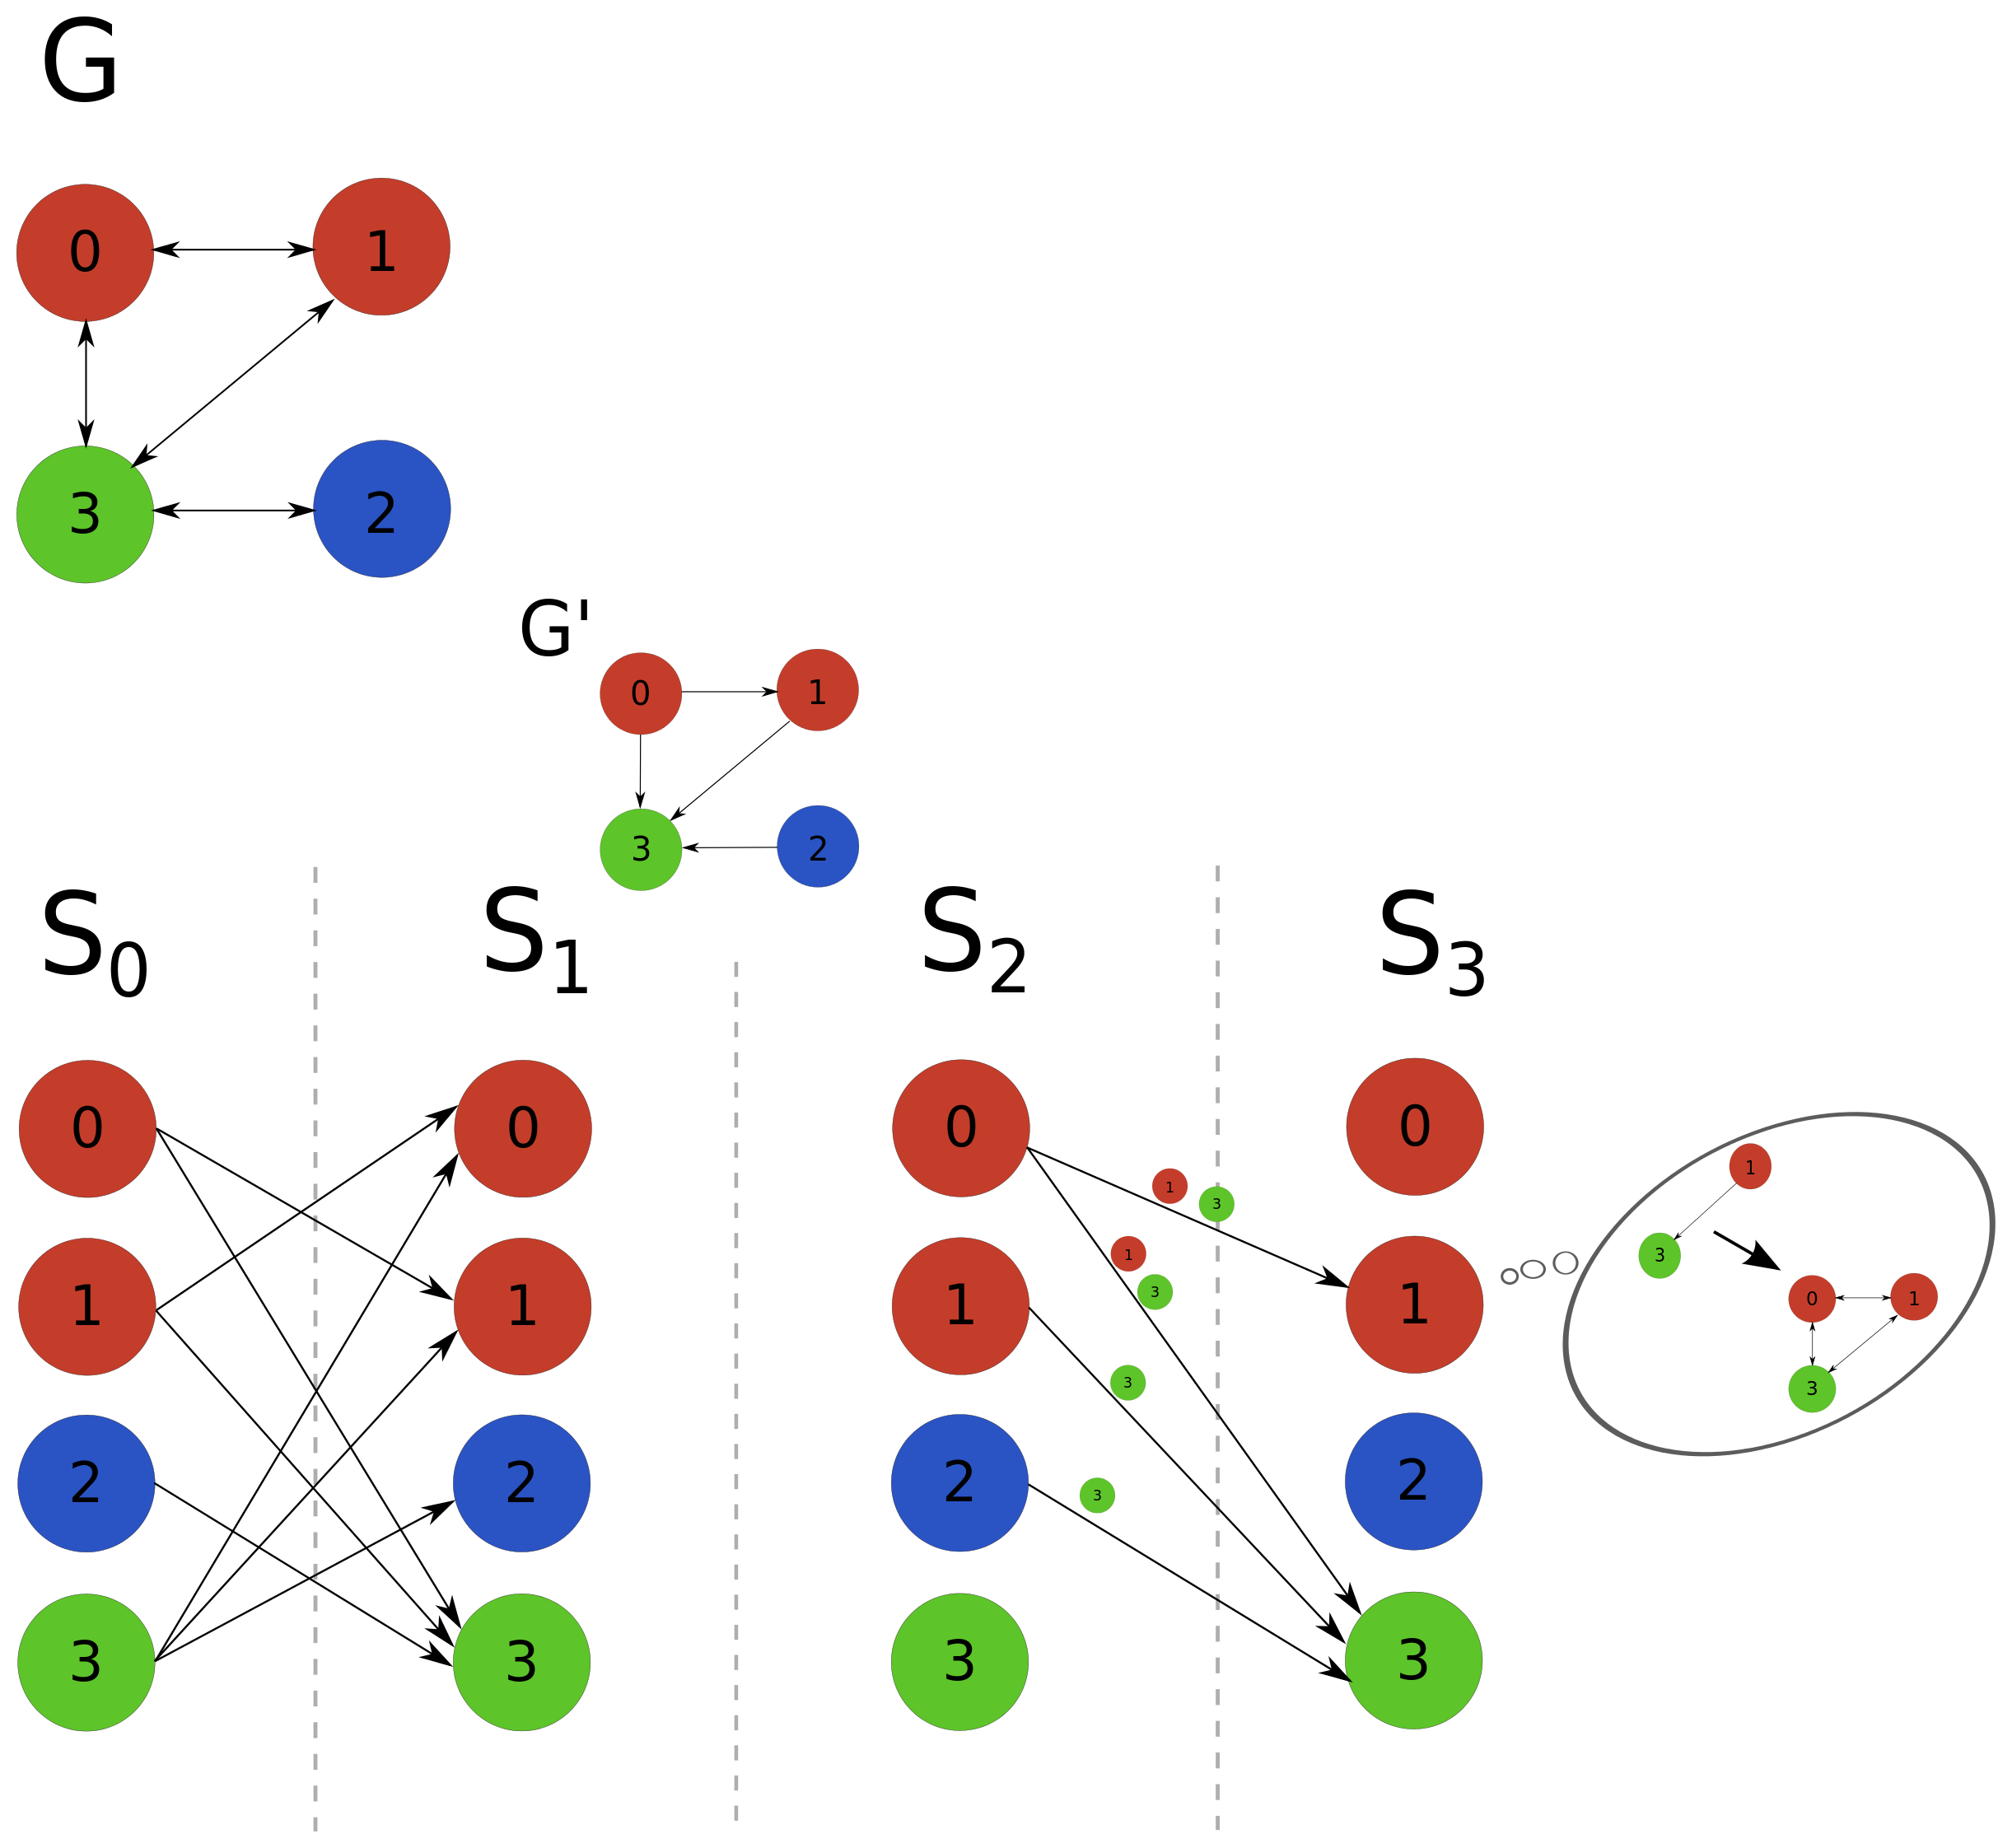
\includegraphics[width=0.8\textwidth]{pregel-trianglepp}
\caption{Esempio calcolo NodeIterator++ in Pregel}
\label{fig:PREGELNIT}
\end{figure}

\section{Densest Subgraph , Ricerca del sottografo più denso in grafi non orientati}

L'algoritmo per la ricerca del sottografo più denso \cite{Bahmani:2012:DSS:2140436.2140442} trova il sottografo \textit{G'} del grafo G la cui densità $\rho(G')$ è una  (2 + 2$\epsilon$)-approsimazione di $\rho*(G)$,dove $\rho*(G)$ è la densità maggiore tra i sottografi di G.

L'algoritmo per la  ricerca del sottografo più denso per grafi non orientati prende in input un grafo \textit{G = (V,E)} non orientato e un valore \textit{$\epsilon > 0$}.
L'algoritmo, il cui pseudocodice è mostrato in \ref{lst:densestU} procede in modo iterativo ed ogni iterazione è composta dai seguenti passi:
\begin{enumerate}
\item Il calcolo della densità corrente $\rho$ del grafo G' e di un valore \textit{soglia}. La densità del grafo $\rho(G')$ è definita come \textit{$\rho(G') = |E(G')| / |V(G')|$} mentre il  valore \textit{soglia}  è definito da \textit{$solgia = 2 (1 + \epsilon) \rho(G') $}.

\item Ogni nodo \textit{v} con \textit{deg(v) < soglia}, dove \textit{deg(v)} è il grado del vertice \textit{v} nel grafo \textit{G'}, viene rimosso assieme agli archi ad esso associati ottenendo il grafo \textit{G"}.
\item Se \textit{ |V(G")| > 0}, con \textit{|V(G")|} numero di archi in \textit{G"} allora si ripete l'iterazione dal passo 1, altrimenti l'algoritmo termina e viene restituito in output il sottografo con valore densità $\rho$ maggiore.

\end{enumerate}

In \cite{Bahmani:2012:DSS:2140436.2140442} viene dimostrato che il sottografo \textit{G'} più denso tra i sottografi \textit{G"} ottenuti grazie all'algoritmo è un sottografo la cui densità è $\rho(G")$ è una  (2 + 2$\epsilon$)-approsimazione di $\rho*(G)$, dove $\rho*(G)$ è la densità maggiore tra tutti i sottografi di G.

\begin{minipage}{\linewidth}
\lstinputlisting[style=customc,caption={Pseudocodice Denesest Subgraph per grafi non orientati},label={lst:densestU}]{code/densestU.c}
\end{minipage}

\subsection{MapReduce}

Per realizzare l'algoritmo in \textit{MapReduce} è stato implementata l'idea descritta in \cite{Bahmani:2012:DSS:2140436.2140442}. Ogni iterazione dell'algoritmo viene realizzata in 3 fasi \textit{MapReduce}.


In Figura \ref{fig:MRDENSESETU} è rappresentato un esempio dell'esecuzione di un iterazione dell'algoritmo in MapReduce.

Nella prima fase viene calcolato il grado di ogni nodo \textit{v} del grafo in input. La realizzazione di questa fase è simile all'implementazione di \textit{DegreeCalculator} in \textit{MapReduce}. Contestualmente alla funzione \textit{Map} della prima fase vengono contati anche il numero totale di vertici e di archi del grafo, valore necessario per il calcolo della densità corrente del grafo e del valore \textit{soglia}. 

Tra la prima fase e la successiva è effettuato il controllo  per cui, se il valore densità è il risultato migliore ottenuto fino a quel momento allora viene salvato lo stato del sottografo corrente.

Nella seconda e terza fase \textit{MapReduce} vengono eliminati gli archi \textit{(u, v)} dove almeno uno tra i vertici \textit{u} e \textit{v} è di grado minore del valore \textit{soglia}. 
Nella seconda fase vengono controllati i nodi sorgenti di ogni arco mentre nella terza fase sono controllati i nodi destinazione degli archi.

La funzione \textit{Map} della seconda fase prende in input sia l'input iniziale dell'iterazione dell'algoritmo che l'output generato dalla prima fase \textit{MapReduce}.
\textit{Map} produce in output la coppia \textit{<v, u>} per i dati appartenenti all'input iniziale. Per i dati che arrivano dall'output della prima fase, che sono nel formato \textit{<v, deg(v)>}, viene prodotto in output il valore \textit{<v, \$>} solo nel caso in cui \textit{deg(v) > soglia}. In questo caso il simbolo \$ viene interpretato dalla funzione \textit{Reduce} e significa che gli archi con vertice di origine \textit{v} devono essere mantenuti.

La funzione \textit{Reduce} riceve in input la coppia valori \textit{<v, list(u)>}, dove \textit{list(u)} è la lista di nodi raggiungibili da \textit{v}. Per ogni elemento \textit{$w \in list(u)$}, \textit{Reduce} produce in output la coppia \textit{<v,w>} solo nel caso in cui $\$ \in list(w)$. 

La terza fase \textit{MapReduce} opera in modo simile alla seconda, al posto di prendere in input il grafo iniziale dell'iterazione, prende in input l'output della fase precedente. Per controllare il grado dei nodi destinazione degli archi del grafo, la funzione \textit{Map}, invece di produrre i valori \textit{<v,u>}, produce in output la coppia \textit{<u,v>}. L'output di \textit{Map} per il secondo tipo di input è lo stesso prodotto nella fase \textit{MapReduce} precedente.

Anche la funzione \textit{Reduce} opera in modo simile alla funzione \textit{Reduce} della fase precedente con la differenza che in output, per ogni elemento \textit{$w \in list(u)$}, produce in output la coppia di valori \textit{(w,v)}, sempre soltanto nel caso che sia presente il simbolo \textit{\$} in \textit{list(u)}.


\begin{minipage}{\linewidth}
\lstinputlisting[style=customc,caption={Pseudocodice funzione \textit{Map} fase 2 \textit{MapReduce} di iterazoine Denesest Subgraph per grafi non orientati}]{code/esempioMRfase23MapDensetU.c}
\end{minipage}
\begin{minipage}{\linewidth}
\lstinputlisting[style=customc,caption={Pseudocodice funzione \textit{Reduce} fase 2 \textit{MapReduce} di iterazine Denesest Subgraph per grafi non orientati}]{code/esempioMRfase23ReduceDensetU.c}
\end{minipage}

\begin{figure}
\centering
 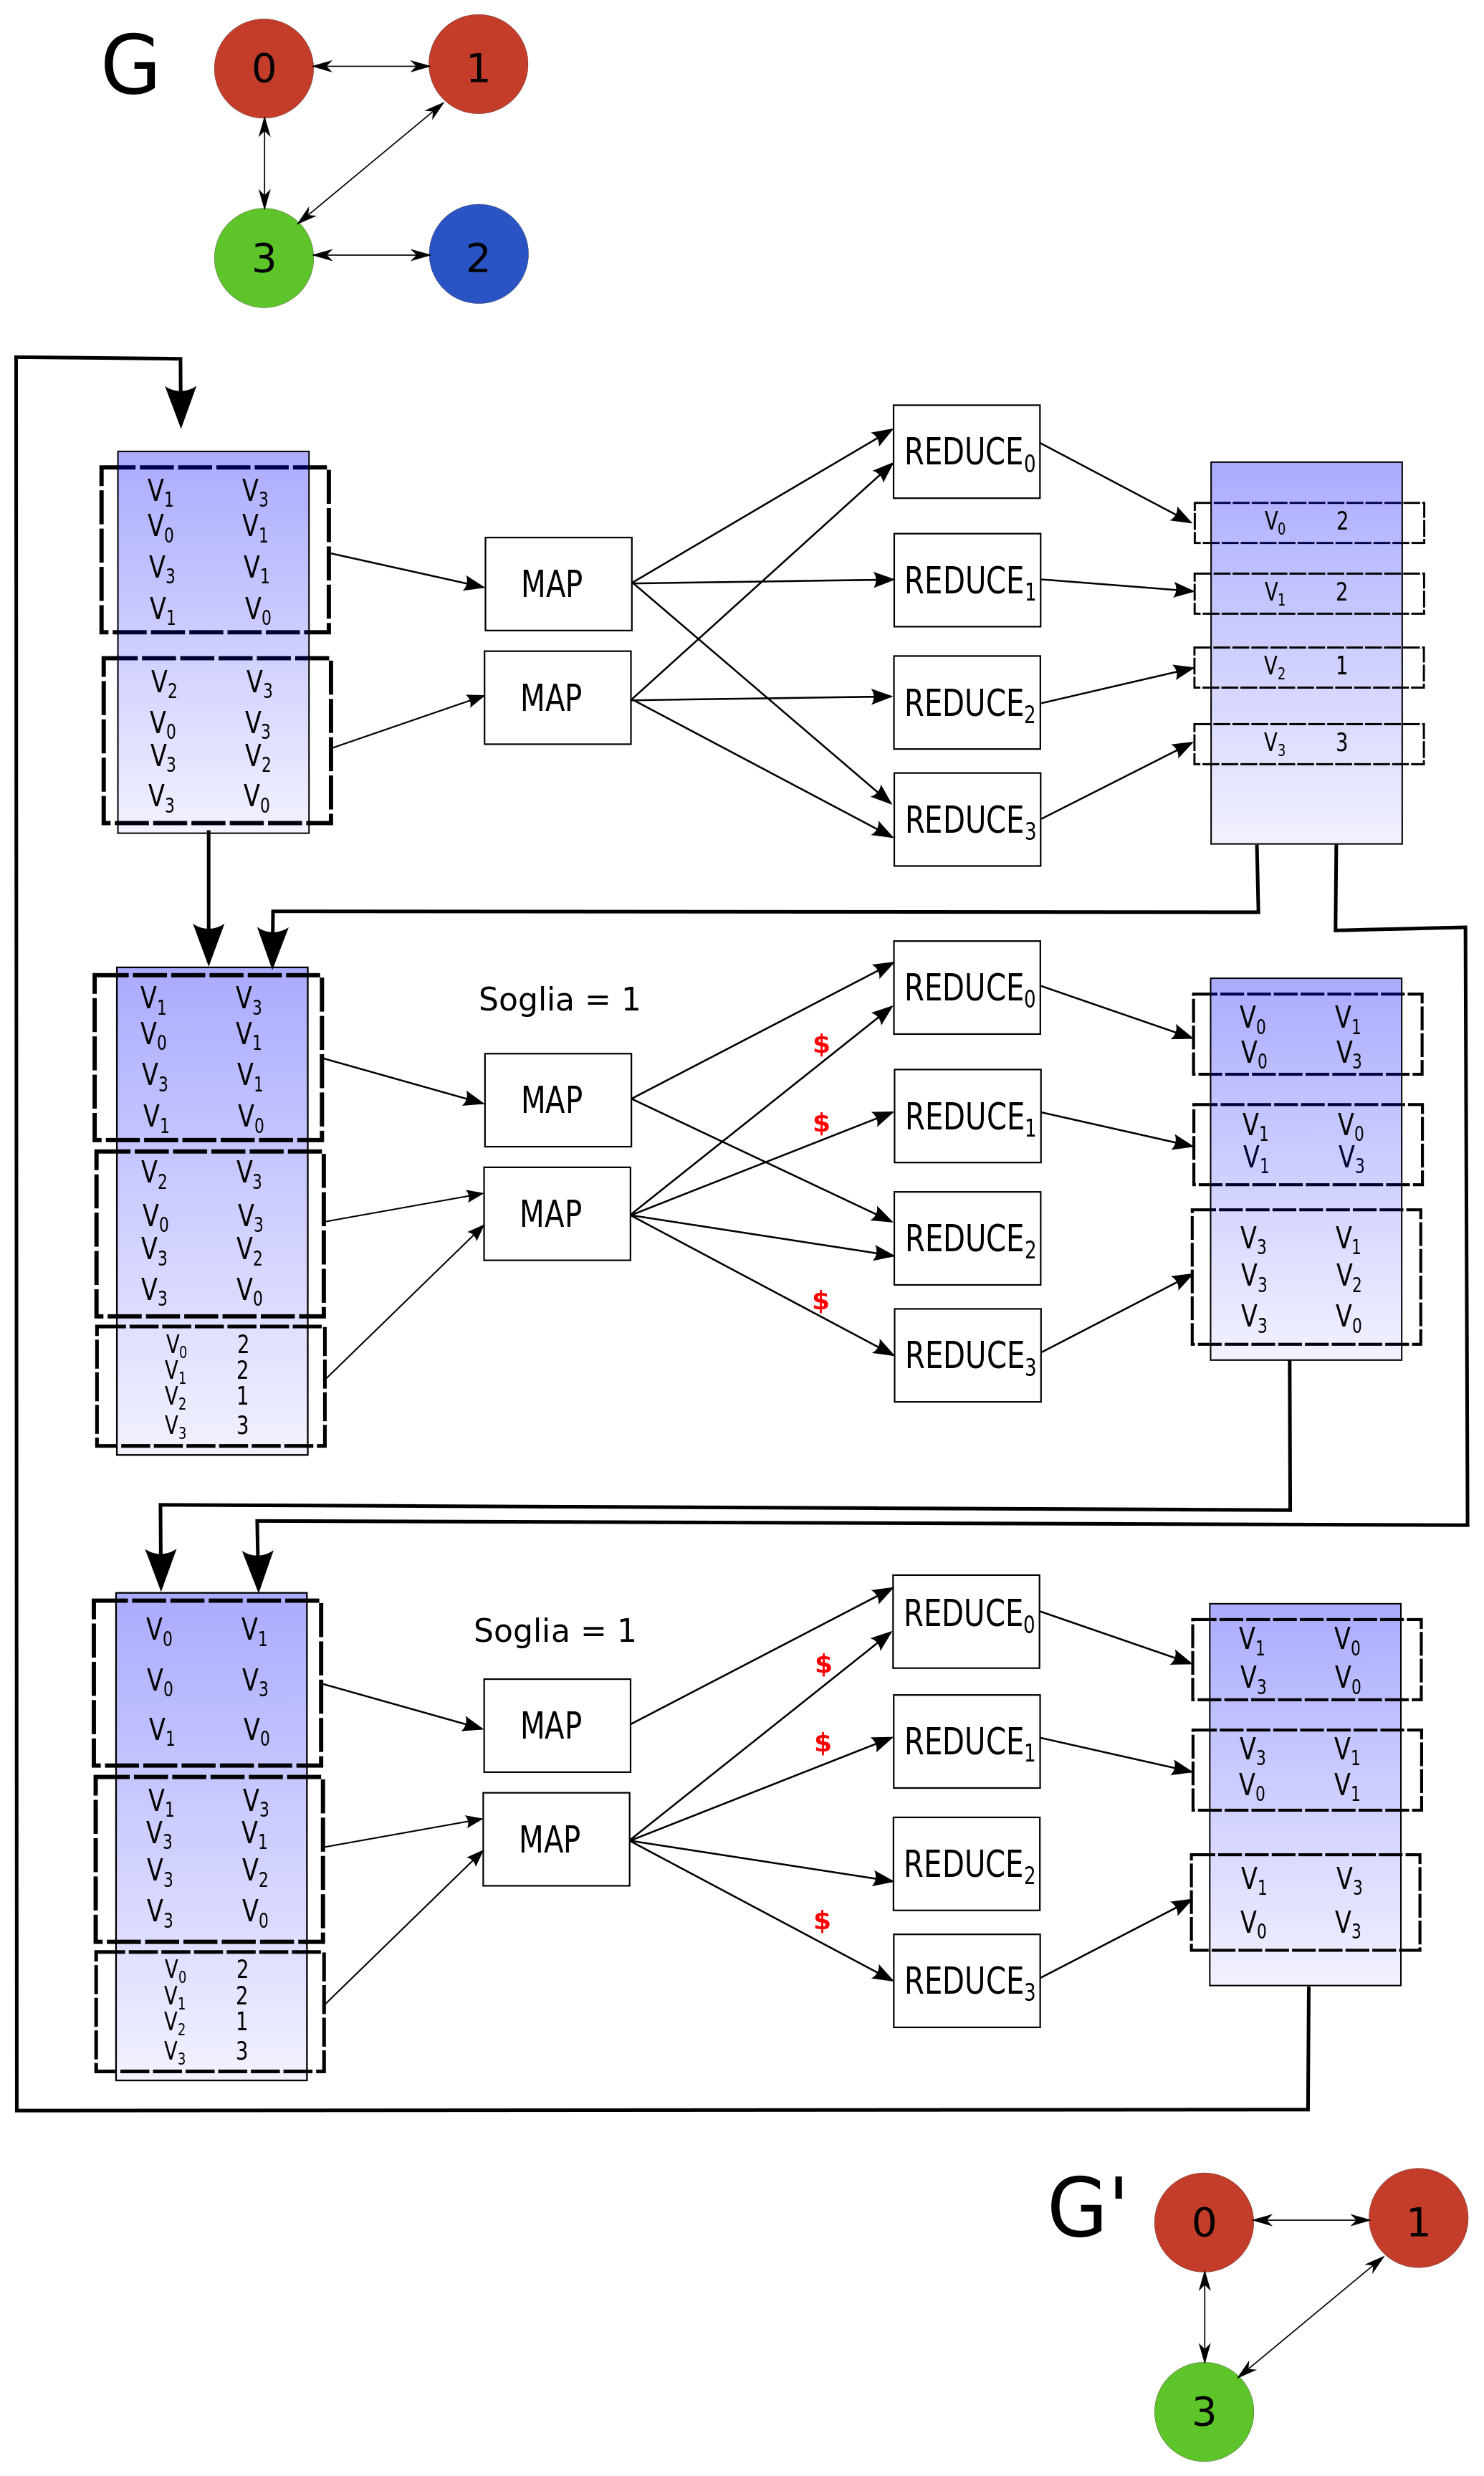
\includegraphics[width=1\textwidth]{MR-denesestU}
\caption{Esempio calcolo Densest Subgraph per grafi non orientati in MapReduce con soglia indicativa}
\label{fig:MRDENSESETU}
\end{figure}




\subsection{Pregel}

Nell'implementazione \textit{Pregel} di \cite{Bahmani:2012:DSS:2140436.2140442}, ogni iterazione dell'algoritmo è composta da due \textit{Superstep}.
Nella Figura \ref{fig:PREGELDENSESETU} è rappresentato un esempio di un'iterazione dell'algoritmo.

Nel primo \textit{Superstep} il vertice \textit{v}, utilizzando le informazioni statistiche del grafo mantenute costantemente dal modello \textit{Pregel}, calcola i valori correnti di densità del grafo, $\rho(G')$, e \textit{soglia}. Se il grado del \textit{v} non rispetta il valore definito dalla \textit{soglia}, cioè se \textit{deg(v) < soglia}, il vertice \textit{v} e tutti gli archi \textit{(v,u)} , di cui il nodo \textit{v} è sorgente, vengono eliminati dal grafo. 
In \textit{Pregel}, come visto in precedenza, gli archi non orientati sono composti da 2 archi orientati e la struttura di ogni arco è mantenuta dal vertice sorgente dall'arco, l'eliminazione di ogni arco viene notificata ai nodi vicini tramite l'invio di opportuni messaggi.
  
Nel secondo \textit{Superstep} i nodi che ricevono i messaggi, che non sono stati già eliminati nel passo precedente, eliminano il verso opposto degli archi eliminati \textit{Superstep} precedente.

Alla fine di ogni iterazione viene controllata la densità corrente dal nodo \textit{Master} definito dell'architettura \textit{Pregel}, ogni volta che si ottiene un valore \textit{densità} migliore viene salvato il sottografo. 

La computazione termina quando non ci sono più vertici attivi nel grafo.

\begin{minipage}{\linewidth}
\lstinputlisting[style=customc,caption={Pseudocodice dell'algoritmo Denesest Subgraph per grafi non orientati}]{code/esempioPregeleDensetU.c}
\end{minipage}


\begin{figure}
\centering
 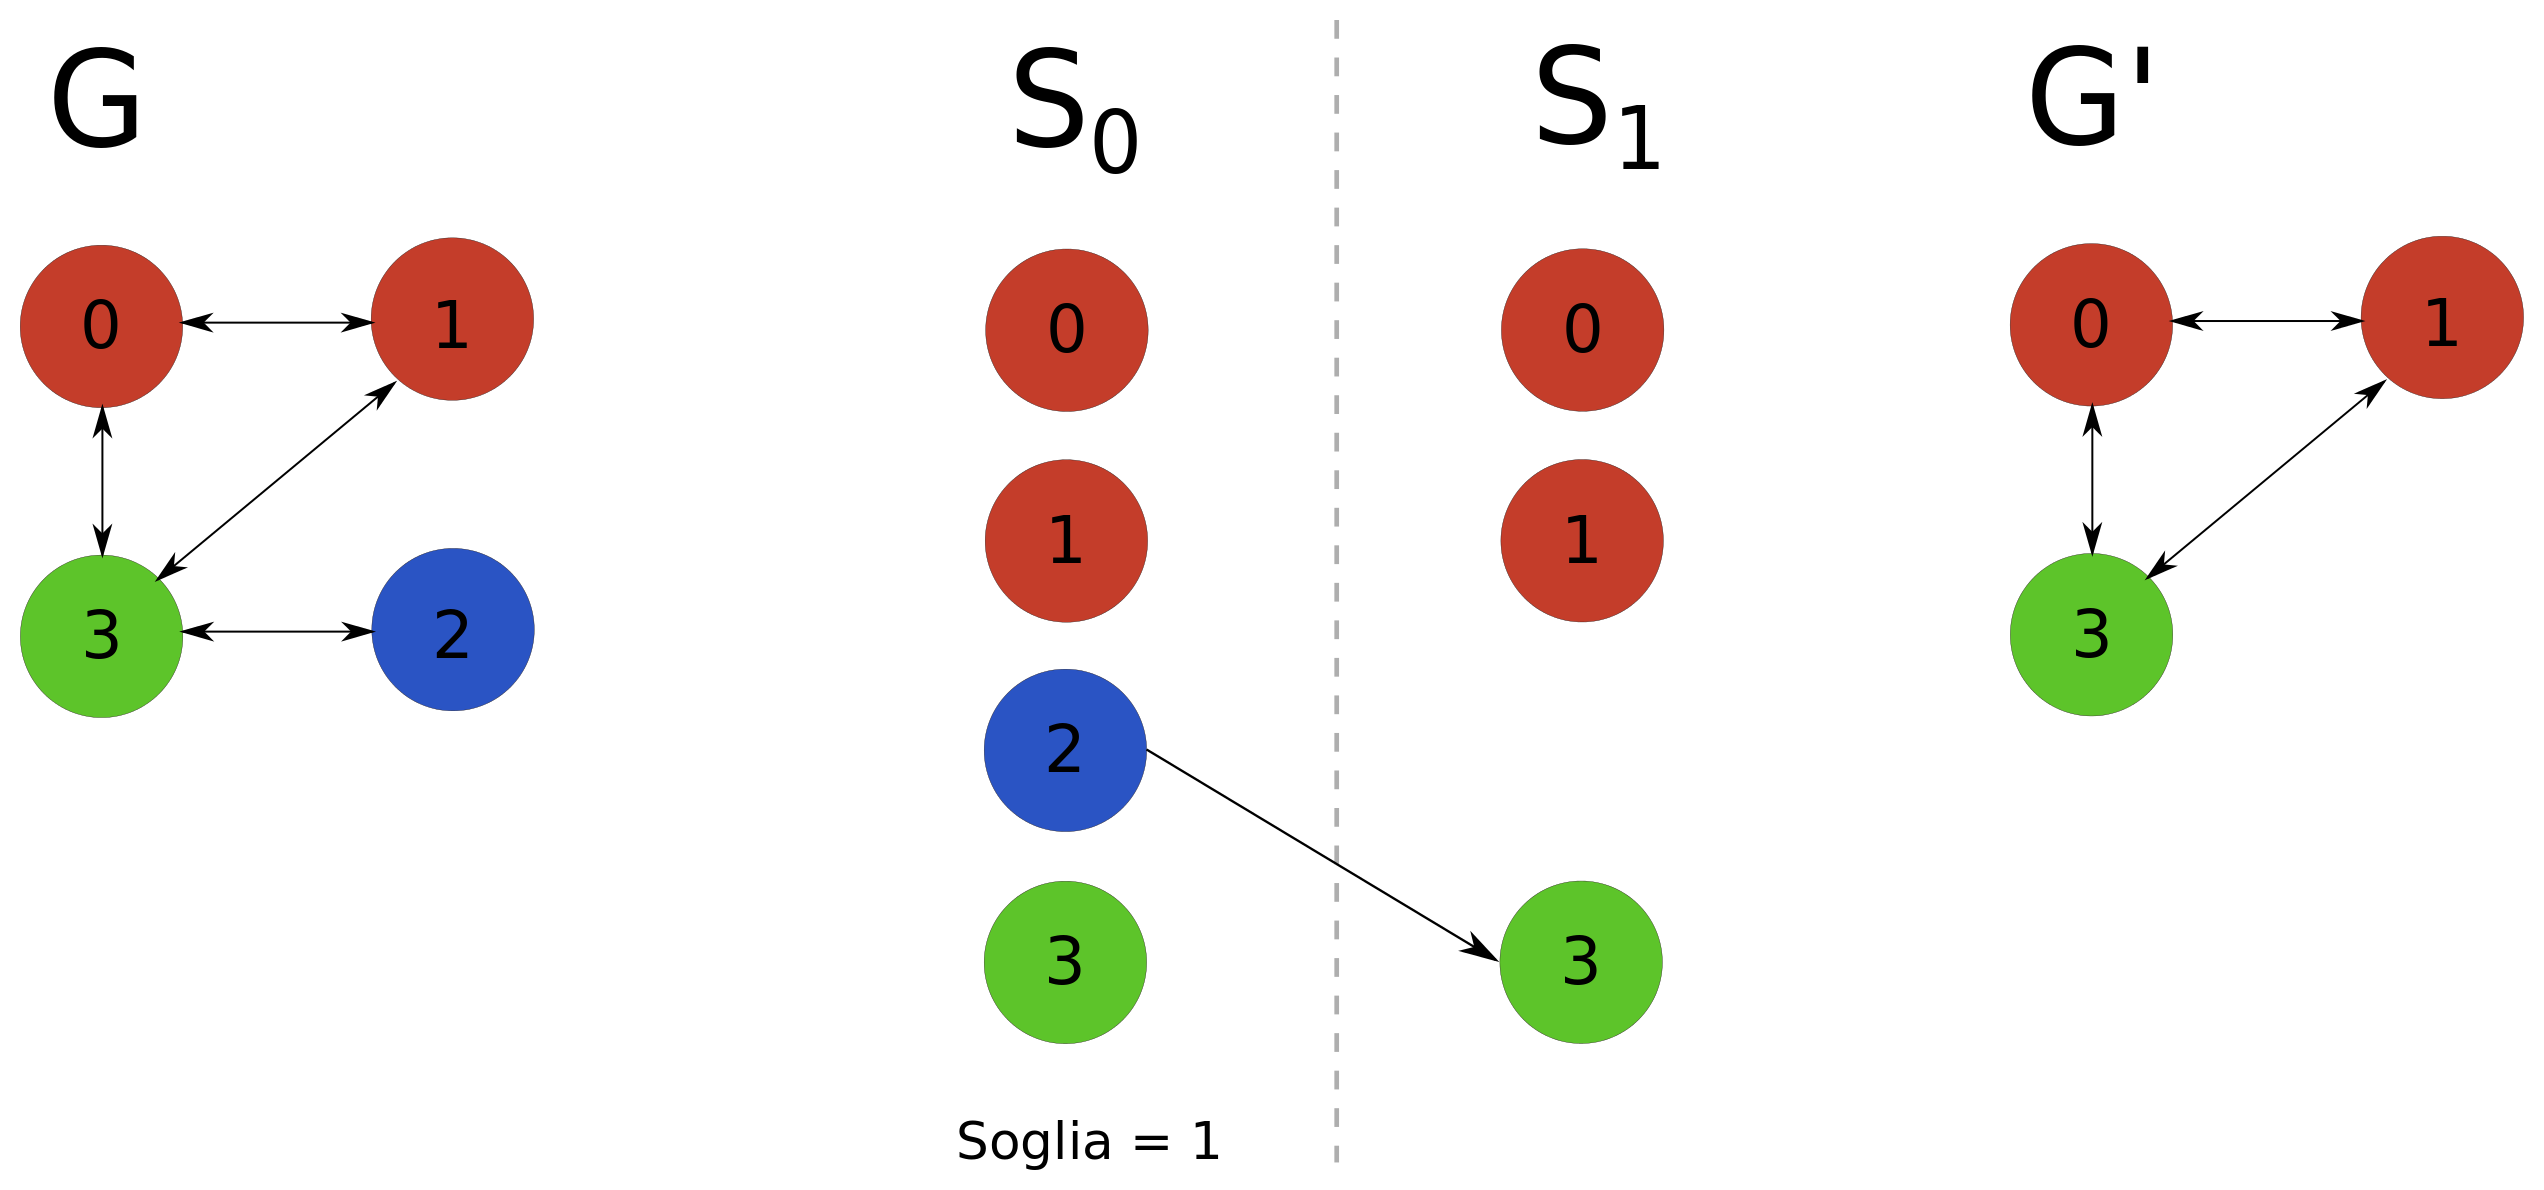
\includegraphics[width=1\textwidth]{PREGEL-denesestU}
\caption{Esempio iterazione Densest Subgraph per grafi non orientati in Pregel}
\label{fig:PREGELDENSESETU}
\end{figure}

\section{Densest Subgraph, Ricerca del sottografo più denso in grafi orientati}

La versione dell'algoritmo per la ricerca del sottografo più denso \cite{Bahmani:2012:DSS:2140436.2140442} per grafi diretti procede in modo simile alla versione per grafi non diretti visto in precedenza. Come per grafi non diretti, l'algoritmo raggiunte, nel caso peggiore, una \textit{2(1+$\epsilon$)-approssimazione} del valore della densità maggiore tra tutti i sottografi del grafo \textit{G}, \textit{$\rho*(G)$}.

L'algoritmo per la  ricerca del sottografo più denso nella versione per grafi orientati prende in input un grafo \textit{G = (V,E)} non orientato, un valore \textit{$\epsilon > 0$} ed un valore \textit{$c > 0$}.
L'algoritmo, il cui pseudocodice è mostrato in  procede in modo iterativo ed ad ogni passo dell'algoritmo:
\begin{enumerate}
\item E' calcolata la densità corrente del grafo \textit{G'}, per un grafo diretto la densità è calcolata come \textit{$\rho(G') = |E(S,T)| /  \sqrt{|S| |T|} $}, con \textit{$S,T \subseteq V$}, $|E(S,T)| = |E| \cap (|S| \times |T|)$. Gli insieme \textit{S} e \textit{T} sono inizializzati come \textit{S = T = V}. Nella Figura \ref{fig:DENSESET} è mostrato un esempio di come vengono ripartiti i vertici del grafo \textit{G} sugli insieme \textit{S} e \textit{T}.
\item Se \textit{|S| / |T| > c} allora vengono eliminati vertici dall'insieme S nel caso in cui il grado uscente del vertice è minore del valore \textit{soglia}, altrimenti vengono eliminati vertici dall'insieme T nel caso in cui grado entrante del vertice è minore del valore \textit{soglia}.
Nel primo il valore di soglia viene calcolato come \textit{$soglia = (1 + \epsilon) |E(S,T)| / |S|$} mentre nel secondo caso viene calcolato come \textit{$soglia = (1 + \epsilon) |E(S,T)| / |T|$}.
\item Se nel grafo \textit{G"} ottenuto dopo l'eliminazione dei vertici nel passo precedente, sono ancora presenti vertici in una degli insieme S o T, l'iterazione dell'algoritmo ricomincia dal passo 1.
\end{enumerate}

In \cite{Bahmani:2012:DSS:2140436.2140442} viene dimostrato che uno dei grafi \textit{G"} ottenuti nel corso dell'algoritmo  è una \textit{(2$\epsilon$ + 2)-approssimazione} del sottografo più denso del grafo iniziale \textit{G}.

\begin{figure}
\centering
 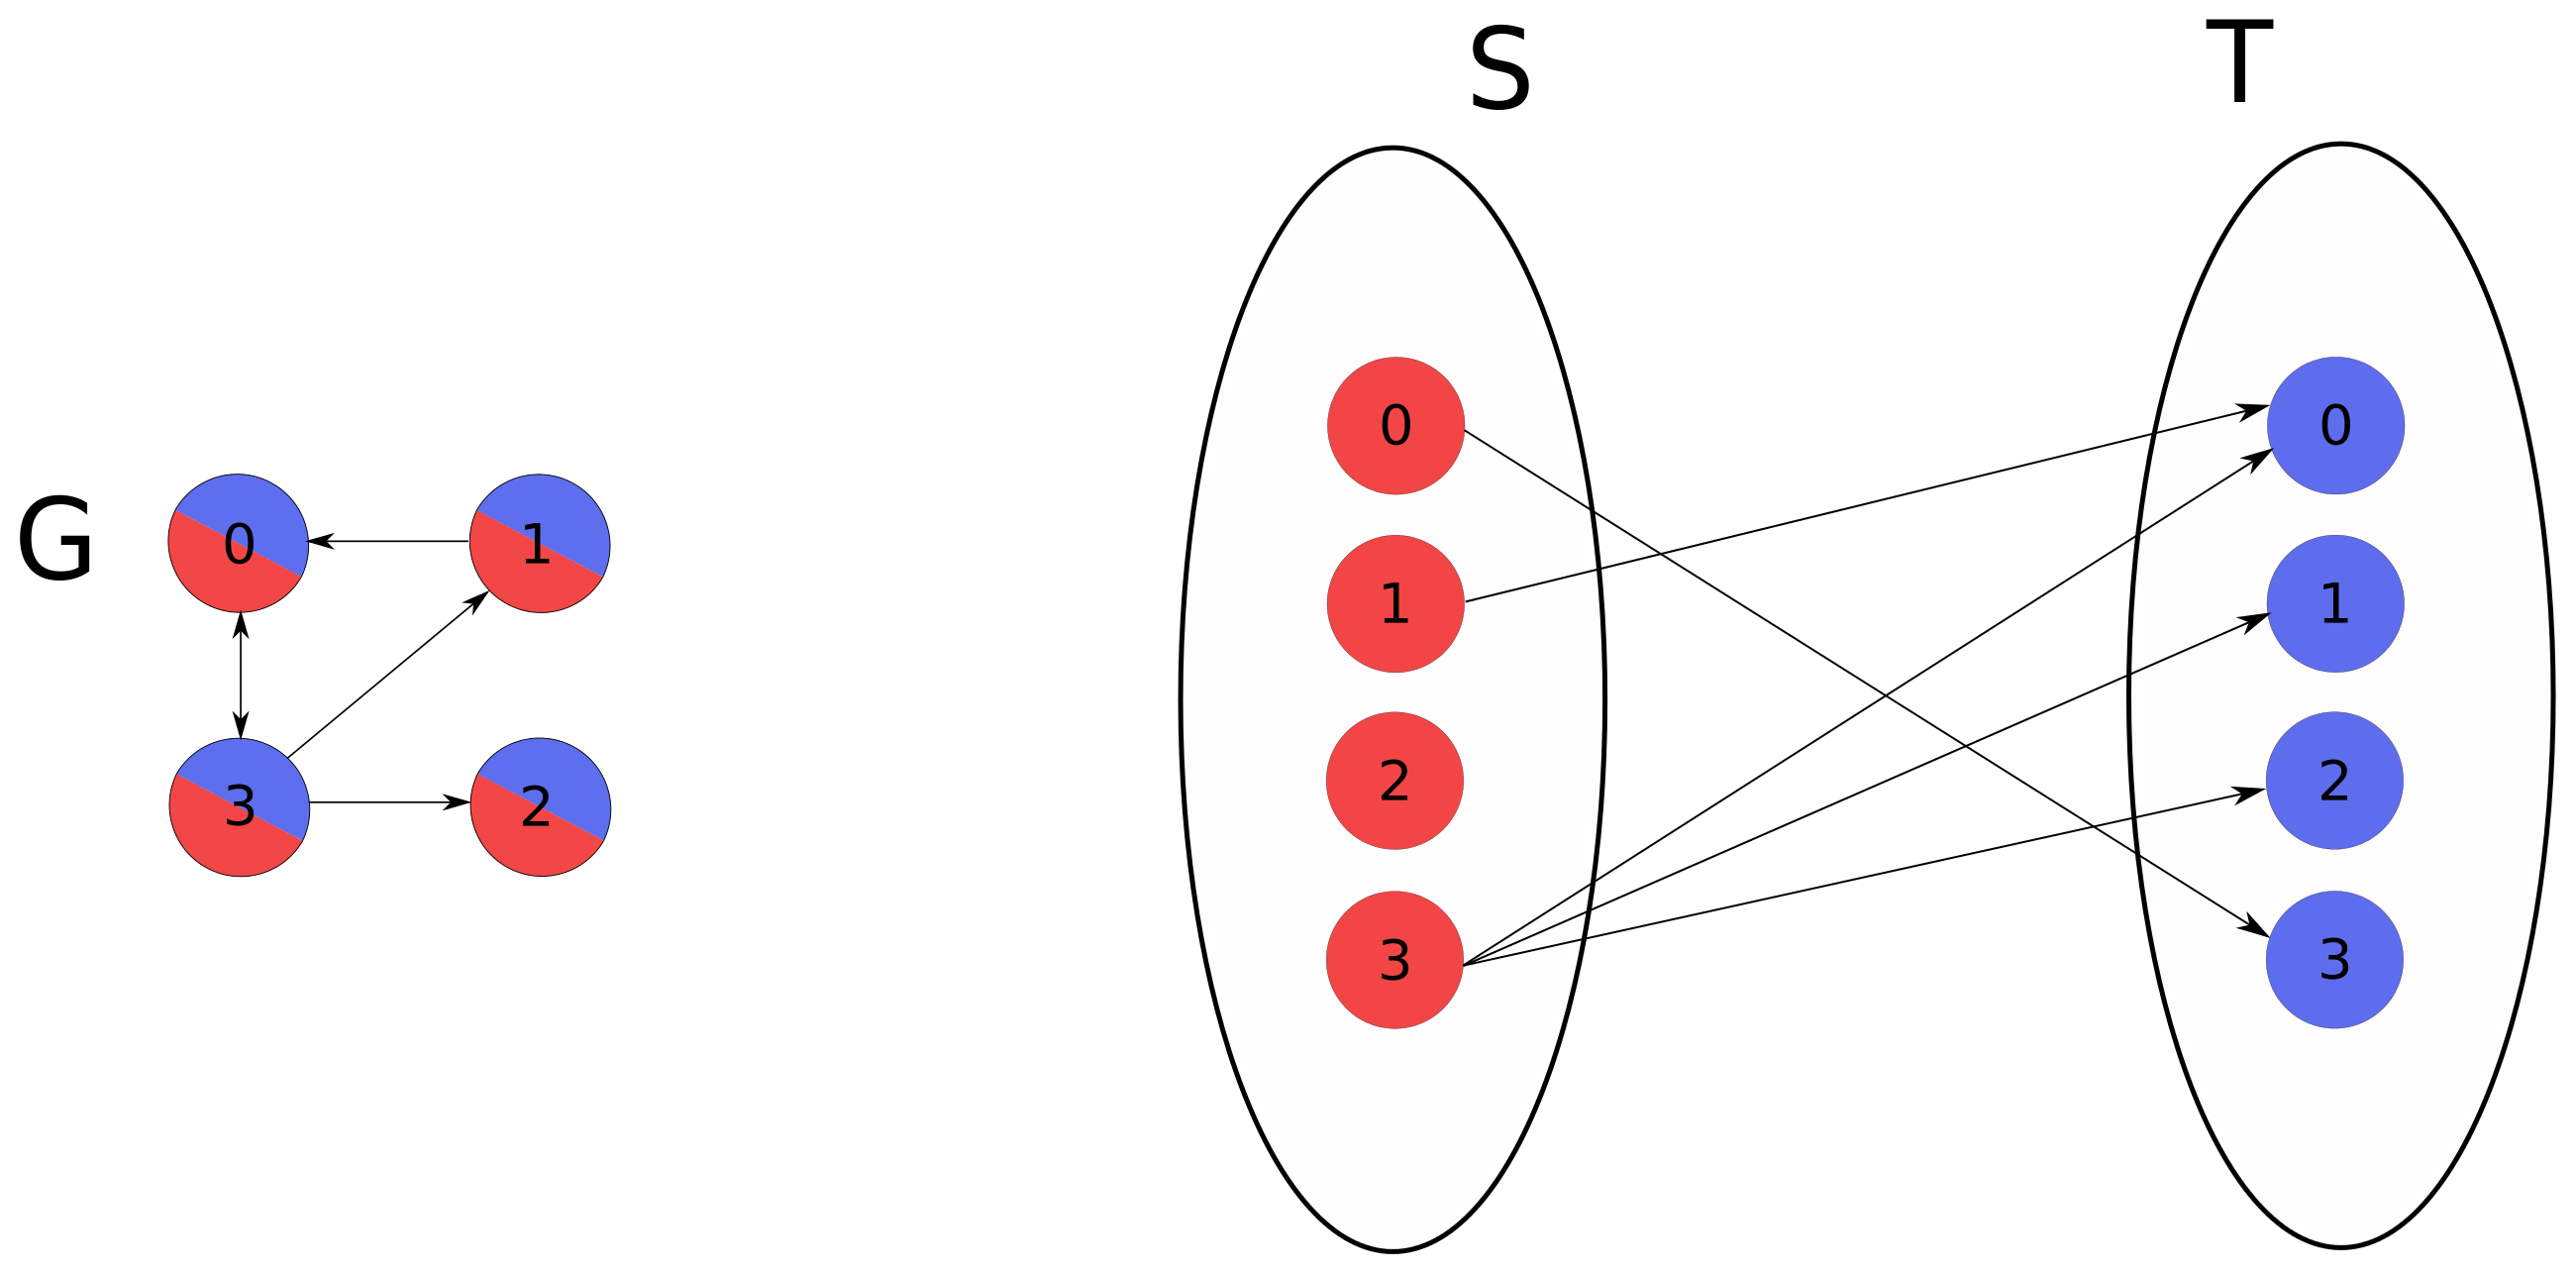
\includegraphics[width=1\textwidth]{denesestD}
\caption{Esempio ripartizione vertici di \textit{G} sugli insiemi\textit{ S} e \textit{T} }
\label{fig:DENSESET}
\end{figure}

\begin{minipage}{\linewidth}
\lstinputlisting[style=customc,caption={Pseudocodice Denesest Subgraph per grafi orientati},label={lst:densestD}]{code/densestD.c}
\end{minipage}

\subsection{MapReduce}

Ogni iterazione dell'algoritmo per la ricerca del sottografo più denso in grafi orientati è stata sviluppata attraverso 3 iterazioni \textit{MapReduce}. Nelle prime due iterazioni è calcolato il grado uscente dei vertici che si trovano nell'insieme S ed il grado entrante dei vertici che appartengono all'insieme T. La terza iterazione MapReduce varia a seconda che l'algoritmo decida di eliminare vertici dall'insieme S oppure di eliminare i  vertici dell'inseme T.

In Figura \ref{fig:MRDENSESESTD} è rappresentato un esempio di iterazione in \textit{MapReduce} dell'algoritmo.

Entrambe le funzioni \textit{Map}  delle prime due iterazioni \textit{MapReduce} prendono in input la coppia di valori \textit{<v,u>} relativi agli archi del grafo G. Nel primo caso, in cui è calcolato il grado uscente dei vertici nell'insieme \textit{S}, \textit{Map} restituisce in output la coppia di vertici \textit{<v,u>}. Nella seconda iterazione, in cui è calcolato il grado uscente dei vertici in \textit{T}, l'output della funzione \textit{Map} è \textit{<u,v>}.

Le funzioni \textit{Reduce} relative alle prime due fasi \textit{MapRedce} ricevono valori in input nel formato \textit{<v,list(u)>}, dove \textit{list(u)} sono i nodi  \textit{u} del grafo corrente collegati da un arco (entrante o uscente) al vertice \textit{v}. L'output restituito dalla funzione è \textit{<v, deg(v)>} dove \textit{deg(v)} è il numero di vertici in \textit{list(u)}, che rappresenta, a seconda della fase \textit{MapReduce} il grado entrante o uscente di \textit{v}.

Contestualmente alle prime due fasi vengono contati il numero di vertici presenti nei due insieme, \textit{|S|} e \textit{|T|}, ed il numeri di archi \textit{|E(S,T)|}. Inoltre è calcolato la densità $\rho(G')$ dove \textit{G'} è lo il sottografo corrente. Nel caso $\rho(G')$ è il valore densità più alto rilevato fino a quel momento viene salvato lo stato di \textit{G'}.

Se \textit{|S| / |C| > c} allora è eseguita l'iterazione \textit{MapReduce} che elimina vertici dall'insieme \textit{S}, altrimenti è eseguita l'iterazione \textit{MapReduce} in cui sono eliminati vertici dall'insieme \textit{T}. Entrambe le iterazione prendono due differenti tipi di dati in input:l'input iniziale contente la lista di archi del grafo G, nella forma <v,u>, e uno degli output generati da una delle due iterazioni precedenti in cui sono calcolati rispettivamente il grado dei nodi degli insiemi \textit{S} e \textit{T}, a seconda di qual'è l'insieme in cui si andrà a verificare il grado dei vertici.
%l'output in entrambi i casi e nella forma \textit{<v,deg(v)>}, dove \textit{deg(v)} indica, a seconda dei casi, il grado uscente o entrante di \textit{v}. 
La funzione \textit{Map} per il primo input (nel formato \textit{<v, u>}) restituisce in output la coppia di valori <\textit{v,u}> nel caso in cui siano controllati i vertici in \textit{S} ( \textit{<u,v>} nel caso siano controllati i vertici nell'insieme \textit{T}). 
Per il secondo  input (nel formato \textit{<v, deg(v)>}) se \textit{deg(v) < soglia} viene generato in output la coppia di valori <v, \$>, dove \$ è un valore segnaposto. \$ ha la funzione di segnalare alla funzione \textit{Reduce} che il vertice \textit{v} ha un grado maggiore del valore \textit{soglia} corrente. Il valore \textit{soglia} dipende dall'insieme, \textit{S} o \textit{T}, che è in esame nell'iterazione corrente dell'algoritmo.

La funzione \textit{Reduce} prende in input la coppia di valori \textit{<v, list(u)>} dove list(u) sono i vertici collegati da un arco entrante a \textit{v} nel caso in cui è in esame l'insieme S ( o da un arco uscente nel caso dell'insieme T).
In output la funzione \textit{Reduce} restituisce, per ogni elemento \textit{$w \in list(u)$} i valori \textit{<v, w>} o \textit{<v,w>} nel caso siano in esame, rispettivamente, gli archi uscenti da un nodo in S o gli archi entranti nei nodi in T. In entrambi i casi la funzione \textit{Reduce} restituisce valori solo se il vertice v rispetta la soglia imposta dall'algoritmo, cioè se il valore segnaposto \textit{$\$ \in list(u) $}.

L'iterazione termina quando non ci sono più nodi negli insieme \textit{S} e \textit{T}.


\begin{minipage}{\linewidth}
\lstinputlisting[style=customc,caption={Pseudocodice funzione \textit{Map} della fase 3 \textit{MapReduce} dell'iterazione Denesest Subgraph per grafi non orientati}]{code/esempioMRfase23MapDensetD.c}
\end{minipage}
\begin{minipage}{\linewidth}
\lstinputlisting[style=customc,caption={Pseudocodice funzione \textit{Reduce} della fase 3 \textit{MapReduce} dell'iterazione Denesest Subgraph per grafi non orientati}]{code/esempioMRfase23ReduceDensetD.c}
\end{minipage}


\begin{figure}
\centering	
 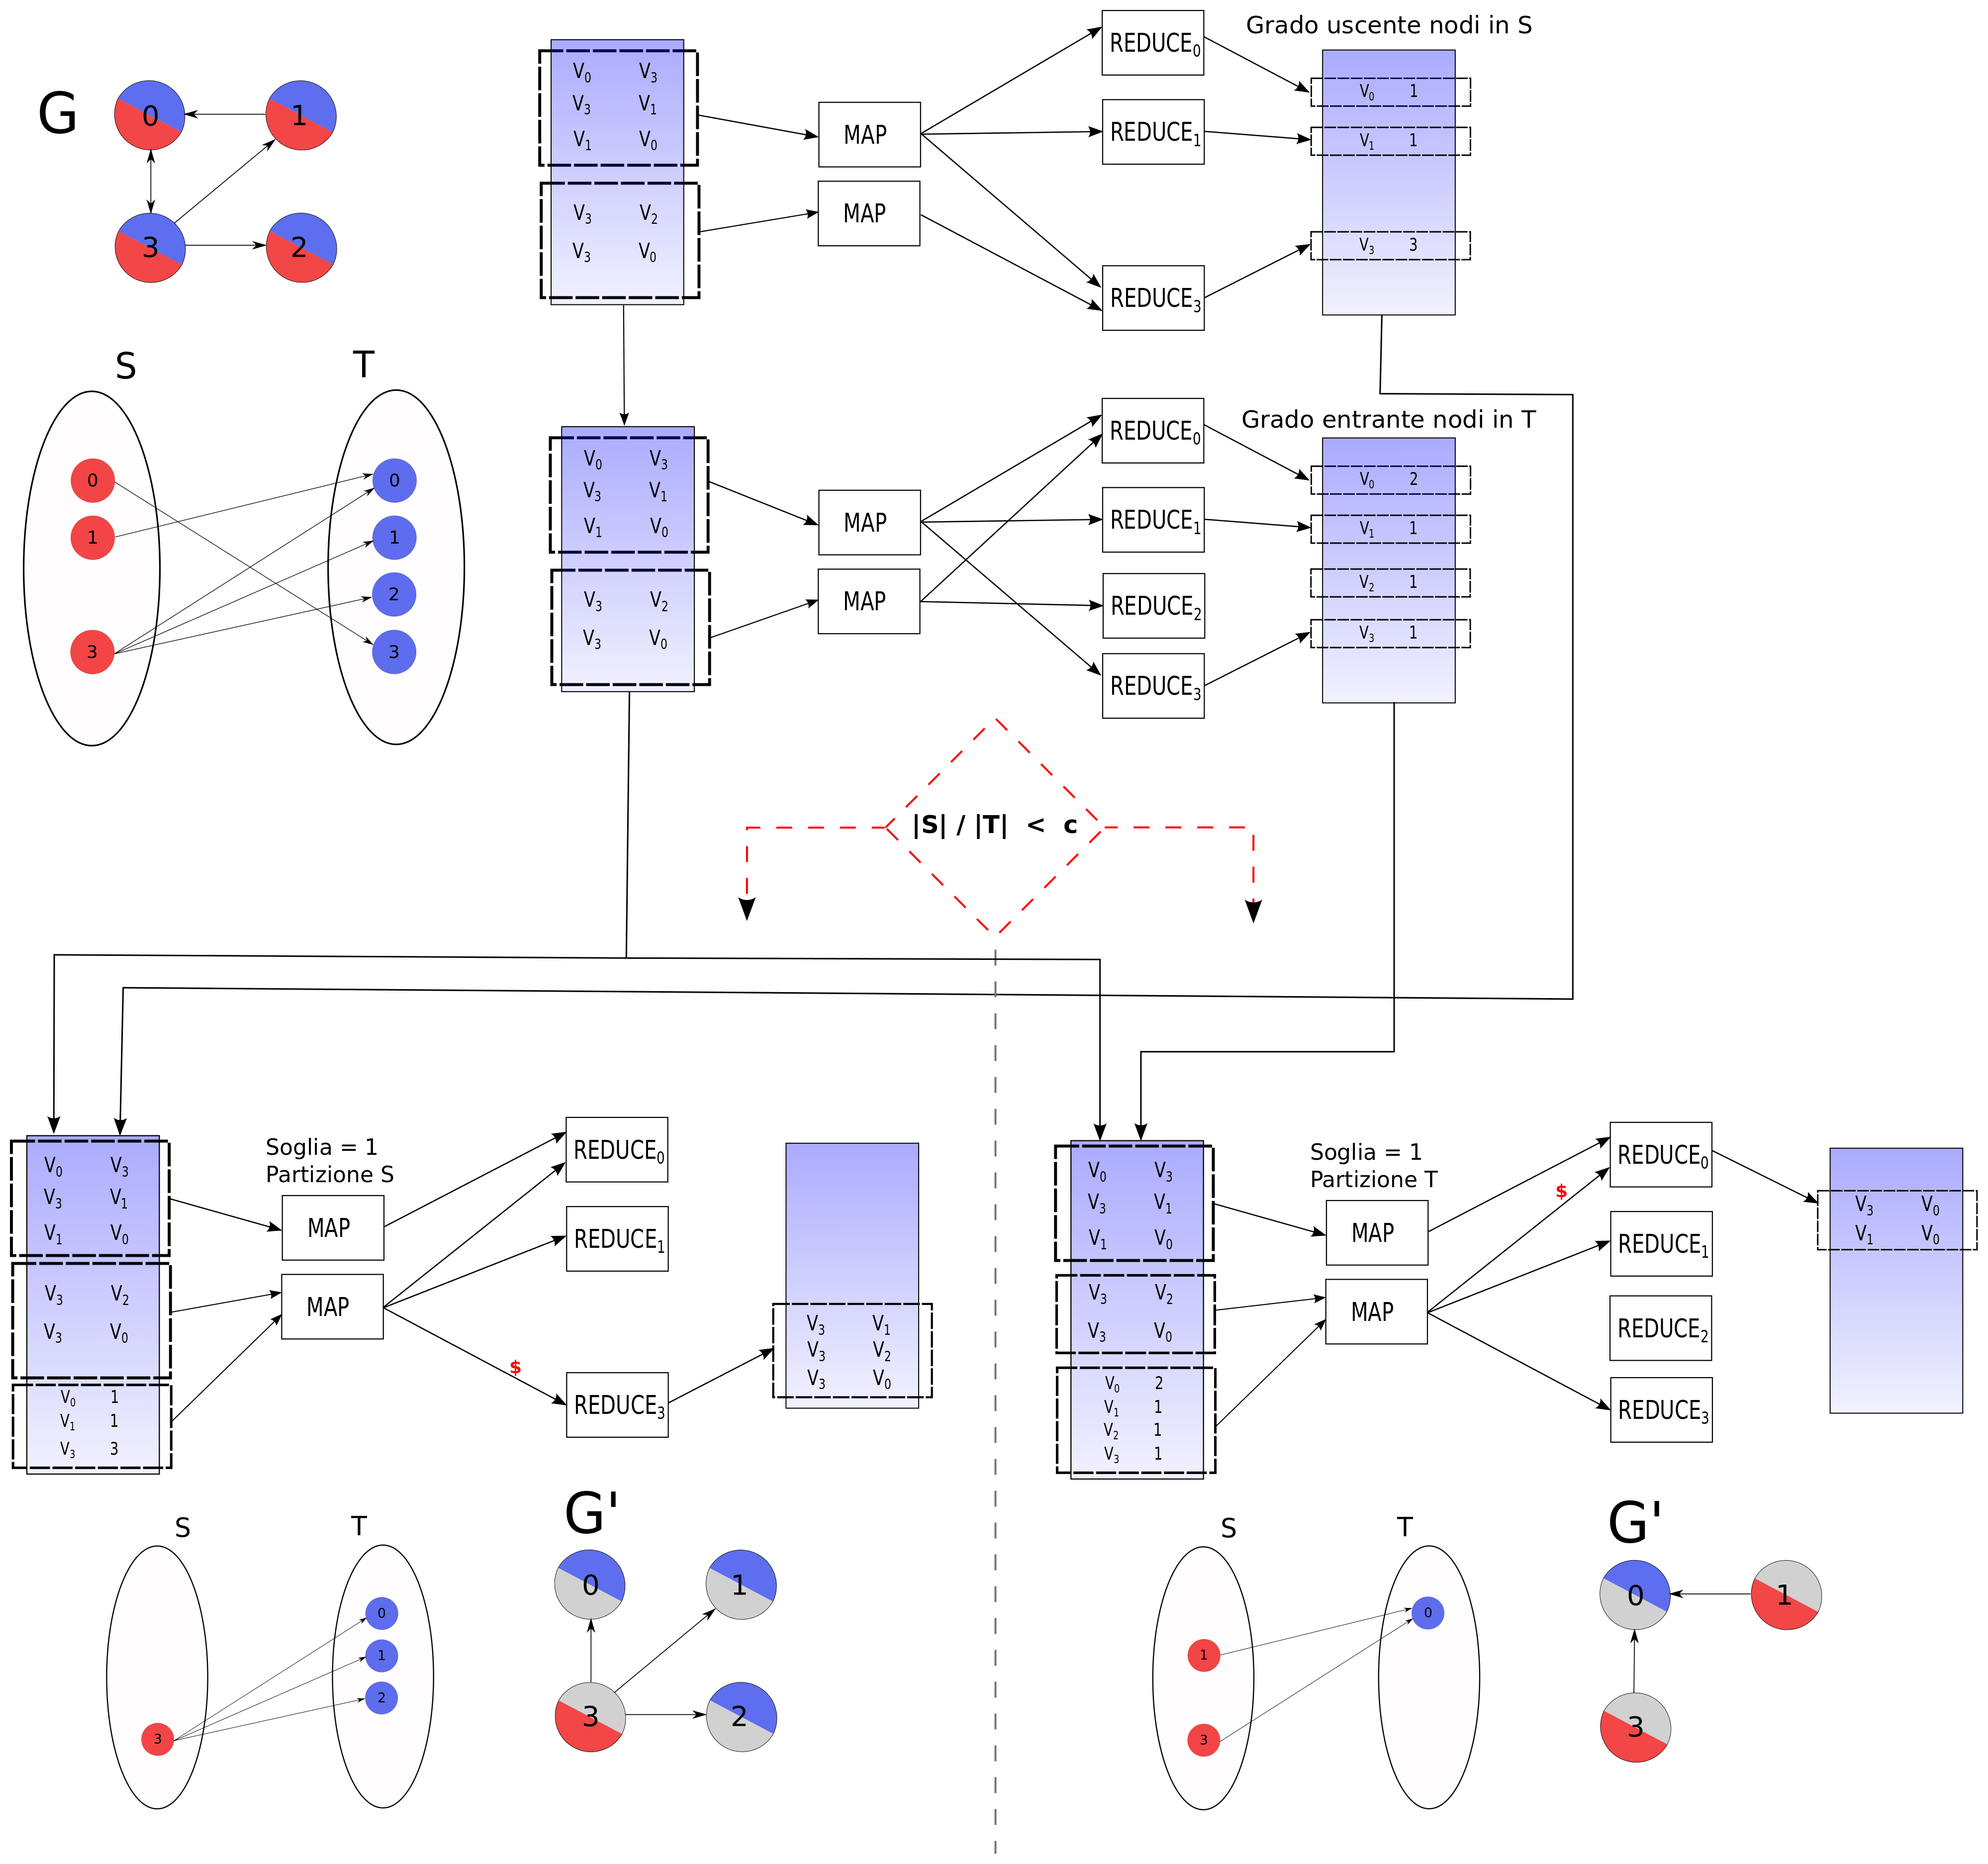
\includegraphics[width=1\textwidth]{MR-denesestD}
\caption{Esempio calcolo Densest Subgraph per grafi orientati in MapReduce}
\label{fig:MRDENSESESTD}
\end{figure}

\subsection{Pregel}

L'implementazione \textit{Pregel} dell'algoritmo prevede la realizzazione di ogni iterazione in due \textit{Superstep}.
 All'inizio di ogni Superstep il nodo Master decide, in base allo stato degli insiemi S e T rilevato tramite sistema di aggregatori, quale funzione \textit{compute} eseguire. Ad ogni Supestep possono essere eseguita la funzione che controlla il grado dei vertici nell'insieme \textit{$v \in S$} o il grado dei vertici nell'insieme \textit{$v \in T$}. 

Il modello \textit{Pregel} prevede che ogni arco del grafo sia associato al vertice \textit{Sorgente} dell'arco. Per poter controllare il grado entrante dei vertici in \textit{T} sono svolti 2 ulteriori\textit{Superstep} di inizializzazione, nel primo \textit{Superstep} ogni vertice invia un messaggio con il proprio valore ID ai nodi vicini. Nel \textit{SuperStep} successivo ogni vertici registra i messaggi ricevuto come arco entrante nella struttura dati associata al vertice.

Nella Figura \ref{fig:PREGELDENSESESTD} è rappresentato un esempio di un iterazione dell'algoritmo in Pregel.

Ad ogni Superstep la funzione \textit{compute} associata al vertice \textit{v} calcola il grado del nodo, entrante o uscente a seconda del caso in cui si trova l'algoritmo. Se il valore è minore della \textit{soglia} corrente allora è eliminato il vertice dalla partizione in esame e tutti gli archi associati.

Nel caso è eliminato un vertice \textit{v} dall'insieme \textit{S}, vengono eliminati gli archi uscenti da \textit{v} e vengono inviati i messaggi ai vertici \textit{u} collegati agli archi eliminati. Nel caso di eliminazione di un arco \textit{v} dall'insieme  \textit{T} allora sono inviati messaggi ai vertici collegati da un arco entrante in \textit{v}. 

I messaggi contengono l'identificativo del nodo \textit{v} eliminato e comunicano al vertice \textit{u} che riceve il messaggio, nel secondo \textit{Superstep} dell'iterazione \textit{Pregel}, di eliminare l'arco associato al vertice \textit{v}. Nel caso che \textit{$v\in S$} allora il vertice \textit{u} elimina l'arco entrante \textit{(u,v)}, nel caso {$v \in S$} allora \textit{u} elimina l'arco uscente \textit{(u,v)}.

Ad ogni iterazione dell'algoritmo è controllata la densità del grafo corrente, nel caso la densità è la maggiore raggiunta dall'algoritmo, viene salvato lo stato del sottografo.


\begin{figure}

\centering
 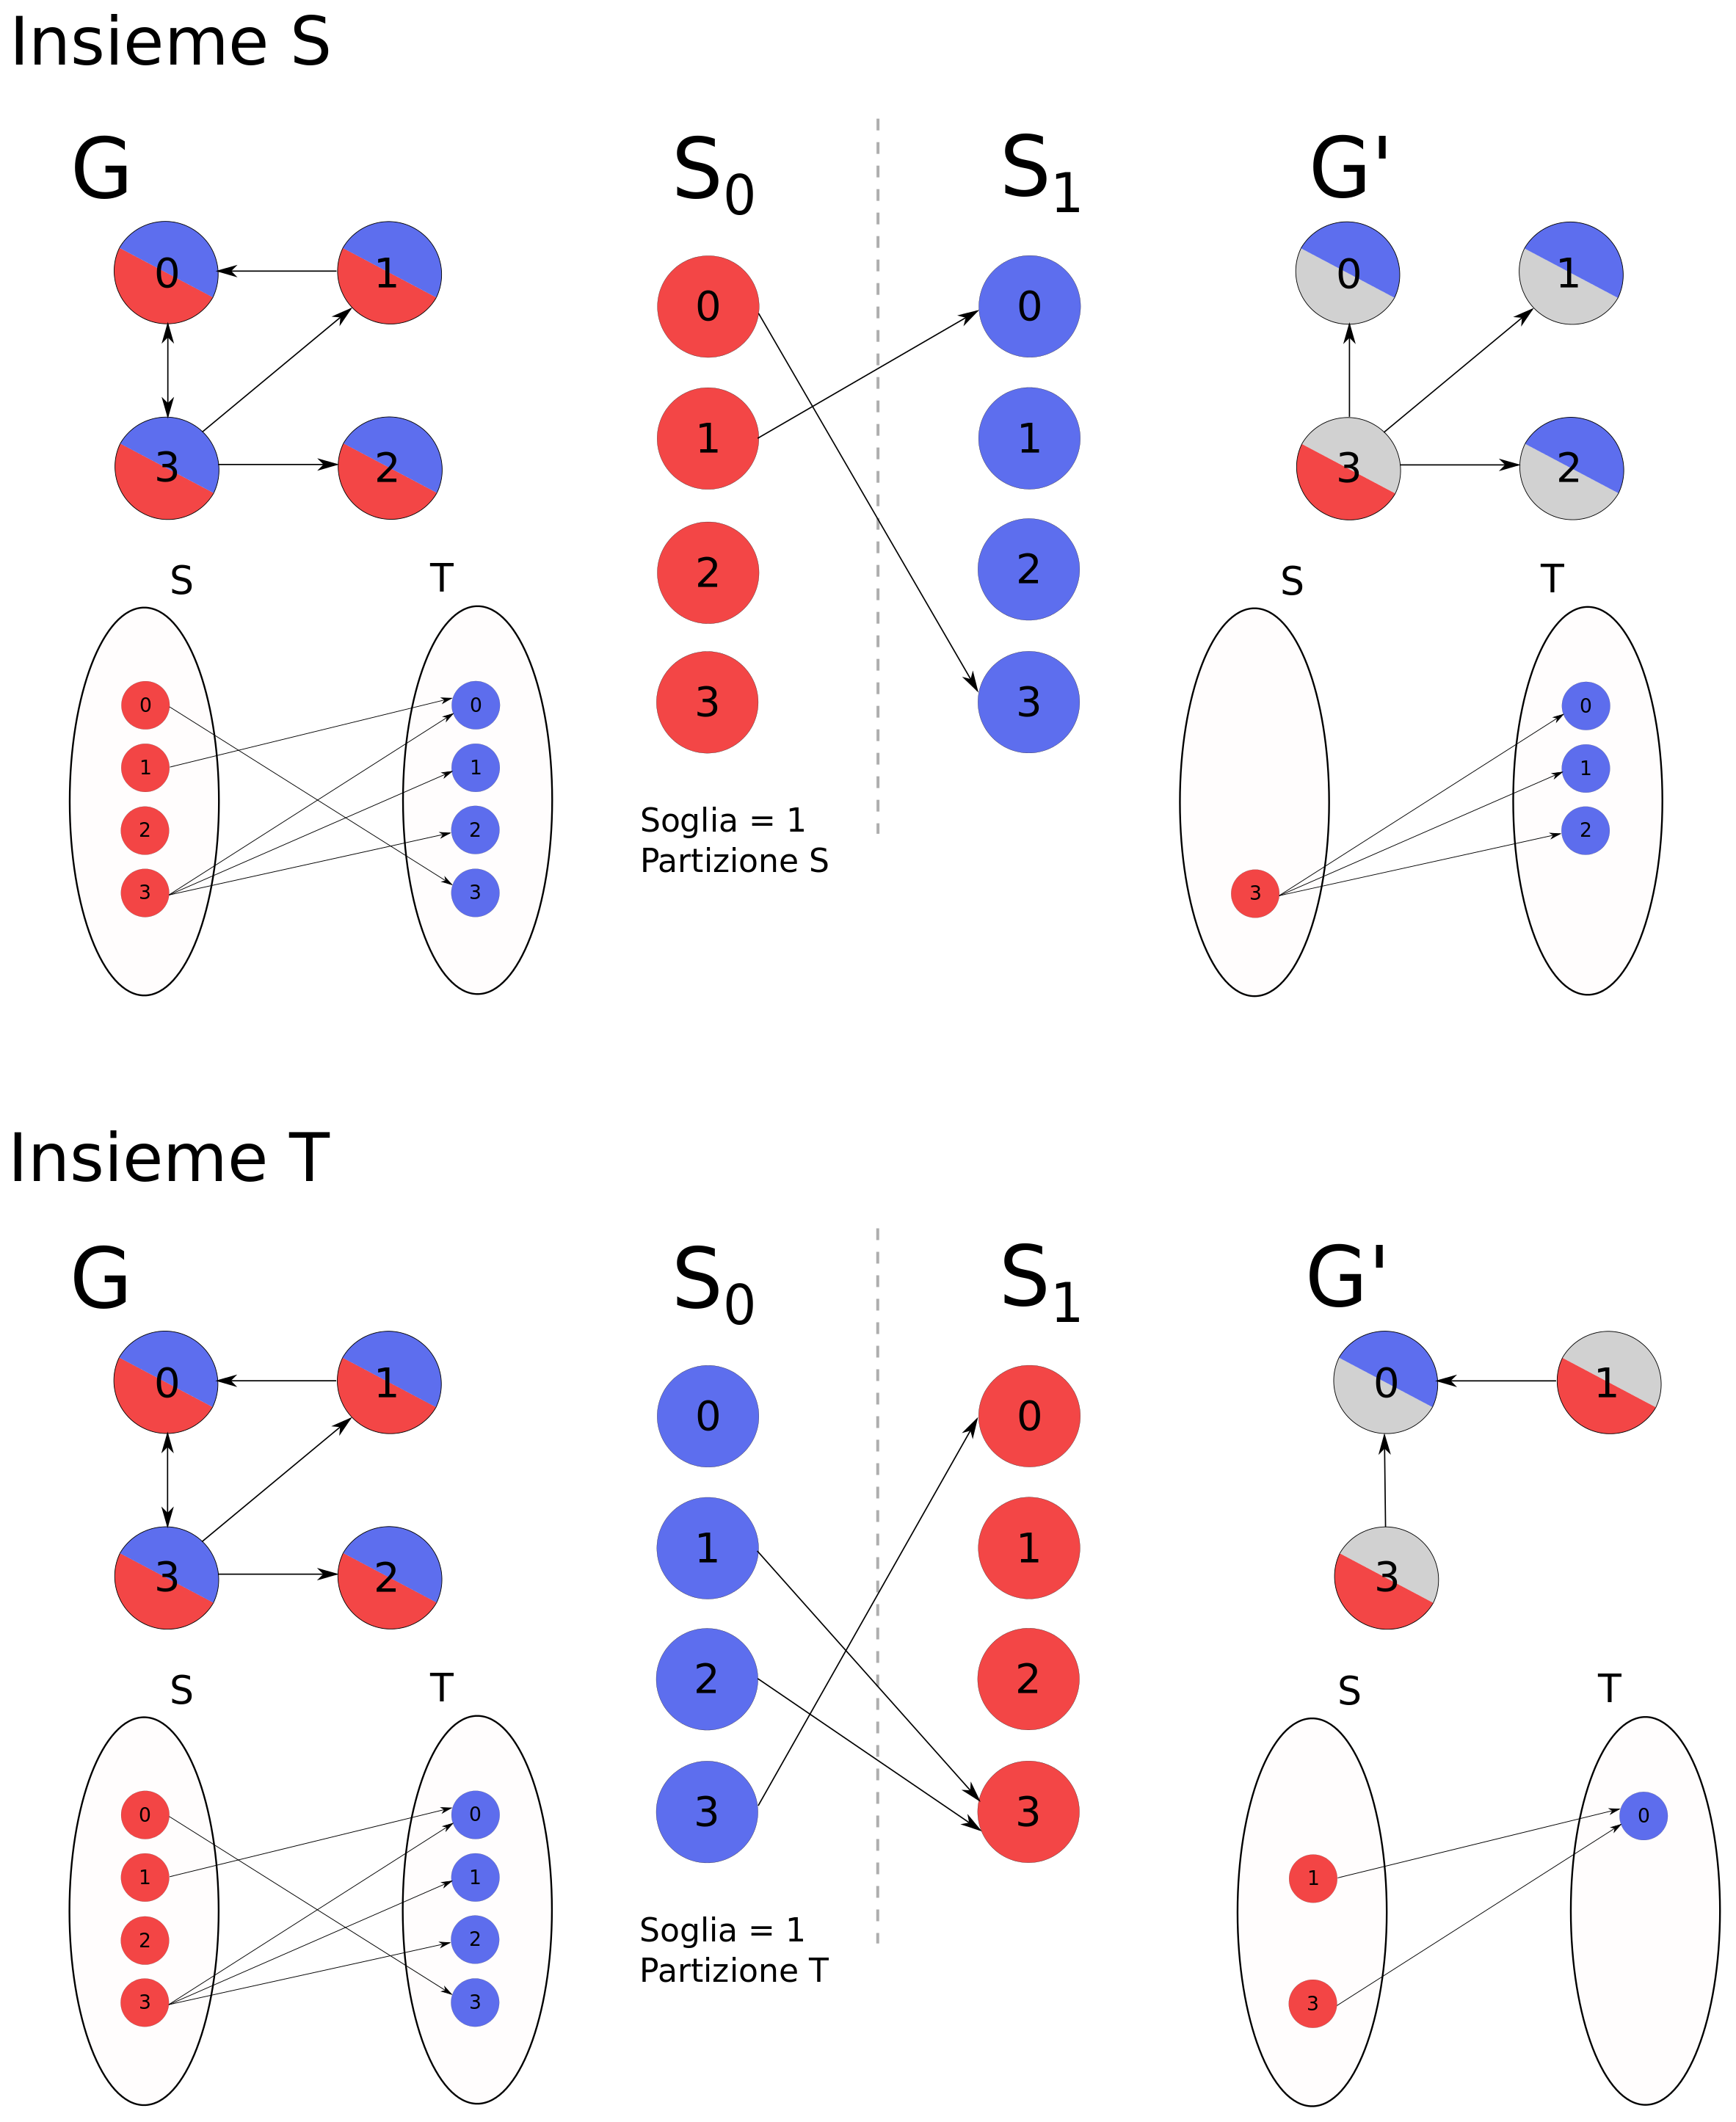
\includegraphics[width=1\textwidth]{PREGEL-denesestD}
\caption{Esempio calcolo Densest Subgraph per grafi orientati in Pregel}
\label{fig:PREGELDENSESESTD}
\end{figure}

\chapter{Test}

Per testare e confrontare i modelli \textit{Mapreduce} e \textit{Pregel}, in questo lavoro di Tesi, sono state eseguite le implementazioni degli algoritmi su \textit{Amazon Web Servicies} (AWS). I risultati ottenuti, dall'esecuzione degli algoritmi sui due modelli, sono stati successivamente analizzati e messi a confronto. 
In questo capitolo verrà prima descritto l'ambiente di test utilizzato e le diverse configurazioni su cui sono stati eseguiti i programmi in Mapreduce e Pregel, verranno descritte successivamente le metriche utilizzate per il confronto delle prestazioni dei due modelli e la metodologia utilizzata per raccogliere i dati necessari. Successivamente verranno mostrati i risultati ottenuti e un analisi delle conclusioni scaturite dal confronto fra i due modelli.

\section{Test}

In questa sezione verranno descritti prima i dataset su cui sono stati eseguiti gli algoritmi implementati sui due modelli. Successivamente saranno analizzate le metriche utilizzate per la rilevazione ed il confronto delle prestazioni ottenute dagli esperimenti effettuati. Infine verrà descritto le modalità con cui sono stati eseguiti i test e la raccolta dei dati utili.

\subsection{Dataset}

Sono stati utilizzati tre dataset selezionati in base alla loro dimensione in modo da testare le prestazioni dei vari modelli su scale di input differenti. Tutti i dataset utilizzati sono stati presi da Stanford Large Network Dataset Collection \cite{snapnets}, \textit{SNAP}.  SNAP è una collezione di dataset di grafi che variano di dimensione e tipologia, da grafi di migliaia di nodi fino a grafi composti da milioni di nodi, da grafi relativi a social network a grafi relativi a reti di co-citazione.

Tra i dataset offerti da SNAP sono stati selezionati tre dataset: 

\begin{itemize}
\item \textit{Facebook}  Un sottografo del social network Facebook, composto da 4039 nodi e 88234 archi.
\item \textit{Twitter } Simile al dataset precedente come tipologia, questo dataset è composto da 81306 nodi e 1768149 archi
\item \textit{LiveJournal} Dataset relativo al social network LiveJournal  composto da 4847571 nodi e 68993773 archi.
\end{itemize}

I dataset sono stati scelti in modo da avere dimensione di input di scala differente. In questo modo oltre ad avere un confronto tra le prestazioni dei diversi modelli, è stato possibile ottenere anche un riscontro di come le prestazione di modelli scalano su grafi di diversa dimensione.


\subsection{Metriche}
Per il confronto tra i modelli sono state scelte quattro metriche:
\begin{itemize}
\item Tempo CPU
\item Utilizzo di memoria
\item Scrittura su memoria distribuita
\item Lettura da memoria distribuita
\end{itemize}

Le prime due metriche sono state scelte per avere un riscontro generale sulle prestazioni del modello sugli algoritmi implementati.
Le metriche relative all'utilizzo delle memoria distribuita sono stati scelti per dare risalto al differente utilizzo che i due modelli ne fanno, in particolare modo in relazione ad algoritmi che prevedono un numero elevato di iterazioni.

Come anticipato nel secondo e terzo capitolo, le implementazioni dei modelli utilizzate sono rispettivamente Apache Hadoop \cite{1_hadoop.apache.org_2015} per Mapreduce e Apache Giraph \cite{4_giraph.apache.org_2015} per Pregel. Essendo Apache Giraph costruito sopra l'architettura di Apache Hadoop, è stato possibile sfruttare il report fornito da quest'ultimo per ricavare i valori relativi alle metriche selezionate.

Il \textit{tempo CPU} è calcolato come la somma totale dei tempi di occupazione della CPU da parte dei processi Mapreduce sul totale delle macchine utilizzate nell'elaborazione. Su ogni macchina l'informazione è ricavata dai dati presenti nel file /proc/cpuinfo del sistema operativo Linux utilizzato da AWS.

In modo simile, L'utilizzo della memoria è calcolato come la quantità totale di memoria utilizzata delle macchine coinvolte nel processo. Le informazioni sono ricavate dal file /proc/meminfo  del sistema operativo Linux utilizzato da AWS.

Le metriche che riguardano la lettura/scrittura su memoria distribuita sono anch'esse direttamente acquisibili dal report fornito da Apache Hadoop.  In entrambi i casi, le metriche vengono raccolte in modo incrementale ad ogni attività di lettura/scrittura svolta dai due framework.

\subsection{Metodo}

Per l'esecuzione dei test  si è seguito il seguente metodo:

\begin{itemize}
	\item Per ogni versione dei vari algoritmi, Mapreduce e Pregel, è stato eseguita una fase di test su ciascuno dei dataset selezionati.
	\item Ogni fase di test è composta da tre ripetizioni della stessa elaborazione.
	\item Ogni fase di test è stata due volte su cluster di macchie di dimensione differente.
\end{itemize}


L'esecuzione degli algoritmi su dataset di dimensioni differenti, come detto in precedenza, permette il confronto delle prestazioni dei modelli in rapporto alla dimensione del grafo in input.
Per ogni fase di test si è deciso di ripetere l'esecuzione dell'algoritmo tre volte. I dati utilizzati per il  confronto sono ricavati della media dei valori emersi dalla ripetizione dell'elaborazione.
Infine l'intero set di esperimenti è stato eseguito su due diversi insiemi di macchine, uno composto da otto unità ed uno composto da sedici. Questo ha permesso di ricavare una stima di come le prestazione dei due modelli possano scalare anche in relazione alla dimensione del cluster su cui vengono eseguiti.
%TODO: Aggiungere analisi su come scalano su cluster%

\subsection{Ambiente di test}

Come anticipato, l'ambiente su cui sono stati eseguiti tutti i test è \textit{Amazon Web Servicis (AWS)}. 
AWS è composto da una serie di servizi basati sul cloud altamente configurabili in base alle necessità, in particolare in termini di numero di macchine, di potenza di calcolo, di memoria e di connettività.

Per i nostri test abbiamo utilizzato il servizio \textit{Amazon Elastic MapReduce (EMR)} \cite{1_amazon web services}. EMR 	permette di stanziare cluster  di macchine per l'esecuzione di programmi in Apache Hadoop e quindi anche per Apache Giraph. Per i nostri test abbiamo utilizzato macchine AWS di classe m1.large. Le macchine di classe m1.large sono composte da 4 processori virtuali, 7.8 GB di RAM e 2 instanze da 420 GB di memoria secondaria.




\section{Analisi Performance}


In questa sezione verranno mostrati i risultati ottenuti dai test effettuati. Per ogni metrica verranno confrontate e analizzate le prestazioni ottenute dall'elaborazione degli algoritmi sui due modelli.



\subsection{Tempo CPU}

L'analisi dei risultati ottenuti sul tempo di occupazione totale della CPU ha evidenziato le migliori prestazioni ottenute dagli algoritmi implementati in Pregel. 
In tutti i risultati ottenuti dagli esperimenti svolti è possibile osservare che, all'aumentare delle iterazioni dell'algoritmo sul grafo, il guadagno in termini di occupazione della CPU aumenta.

Infatti è possibile notare nel confonto dei risultati ottenuti per l'algoritmo \textit{DegreeComputation}, rappresentati nelle Figure \ref{tab:degree8} e \ref{tab:degree16}, come la differenza tra l'occupazione della CPU tra i due modelli risulti meno netta rispetto ai risultati ottenuti utilizzando gli altri algoritmi, i quali effettuano  un numero maggiore di iterazioni sul grafo. Come ad esempio avviene in SSSP e Denset Subgraph nella versione per grafi orientati, i cui risultati sono mostrati rispettivamente nelle tabelle \ref{tab:SSSP8} \ref{tab:SSSP16} e  nelle tabelle \ref{tab:DenesestNO8} \ref{tab:DenesestNO16}.

L'unico test in cui è stato rilevato un minor consumo in termini di CPU è quando è stato effettuato il confronto dei risultati sull'algoritmo  DegreeComputation su cluster di 16 macchine e in input il grafo di dimensioni minori, come mostrato nella tabella \ref{tab:degree16}. In questo caso particolare hanno inciso i tempi di inizializzazione maggiore del framework Apache Giraph rispetto a Apache Hadoop. Tali tempi di inizializzazione sono risultati trascurabili rispetto al tempo totale di computazione in tutti gli altri test svolti su  grafi di dimensione maggiore. 


\begin{table}[h!]
\caption{Risultati su occupazione CPU per DegreeComputation su cluster di 8 macchine} 
\label{tab:degree8}
\centering
\begin{tabular}{l l l }
%%GRAPH colum 1
\resizebox {0.32\textwidth}{!}{
\begin{tikzpicture}
\begin{axis} [ylabel={seconds},ybar,ymin=0,ymax=35,xtick=data,ymajorgrids=true,xtick pos=left,x tick label style={rotate=90,anchor=east},xticklabel interval boundaries,symbolic x coords={$Hadoop$,$Giraph$, $EMPTY$},title style={align=center},title={dataset:Facebook}]
\addplot
[ybar interval,fill=blue,draw=black] coordinates{($Hadoop$, 27.117) ($Giraph$, 24.127) ($EMPTY$,0) };\addplot
[ybar interval,fill=red, draw=black] coordinates{($Giraph$, 24.127) ($EMPTY$,0)};
\end{axis}
\end{tikzpicture}
}
&
%%GRAPH colum 2
\resizebox {0.32\textwidth}{!}{
\begin{tikzpicture}
\begin{axis} [ylabel={seconds},ybar,ymin=0,ymax=55,xtick=data,ymajorgrids=true,xtick pos=left,x tick label style={rotate=90,anchor=east},xticklabel interval boundaries,symbolic x coords={$Hadoop$,$Giraph$, $EMPTY$},title style={align=center},title={dataset:Twitter}]
\addplot
[ybar interval,fill=blue,draw=black] coordinates{($Hadoop$, 42.830) ($Giraph$, 34.203) ($EMPTY$,0) };\addplot
[ybar interval,fill=red, draw=black] coordinates{($Giraph$, 34.203) ($EMPTY$,0)};
\end{axis}
\end{tikzpicture}
}
&
%%GRAPH colum 3
\resizebox {0.32\textwidth}{!}{
\begin{tikzpicture}
\begin{axis} [ylabel={seconds},ybar,ymin=0,ymax=700,xtick=data,ymajorgrids=true,xtick pos=left,x tick label style={rotate=90,anchor=east},xticklabel interval boundaries,symbolic x coords={$Hadoop$,$Giraph$, $EMPTY$},title style={align=center},title={dataset:LiveJournal}]
\addplot
[ybar interval,fill=blue,draw=black] coordinates{($Hadoop$, 600.447) ($Giraph$, 303.620) ($EMPTY$,0) };\addplot
[ybar interval,fill=red, draw=black] coordinates{($Giraph$, 303.620) ($EMPTY$,0)};
\end{axis}
\end{tikzpicture}
}
\end{tabular}
\end{table}

\begin{table}[h!]
\caption{Risultati su occupazione CPU per DegreeComputation su cluster di 16 macchine} 
\label{tab:degree16}
\centering
\begin{tabular}{l l l }
%%GRAPH colum 1
\resizebox {0.32\textwidth}{!}{
\begin{tikzpicture}
\begin{axis} [ylabel={seconds},ybar,ymin=0,ymax=65,xtick=data,ymajorgrids=true,xtick pos=left,x tick label style={rotate=90,anchor=east},xticklabel interval boundaries,symbolic x coords={$Hadoop$,$Giraph$, $EMPTY$},title style={align=center},title={dataset:Facebook}]
\addplot
[ybar interval,fill=blue,draw=black] coordinates{($Hadoop$, 42.577) ($Giraph$, 50.893) ($EMPTY$,0) };\addplot
[ybar interval,fill=red, draw=black] coordinates{($Giraph$, 50.893) ($EMPTY$,0)};
\end{axis}
\end{tikzpicture}
}
&
%%GRAPH colum 2
\resizebox {0.32\textwidth}{!}{
\begin{tikzpicture}
\begin{axis} [ylabel={seconds},ybar,ymin=0,ymax=75,xtick=data,ymajorgrids=true,xtick pos=left,x tick label style={rotate=90,anchor=east},xticklabel interval boundaries,symbolic x coords={$Hadoop$,$Giraph$, $EMPTY$},title style={align=center},title={dataset:Twitter}]
\addplot
[ybar interval,fill=blue,draw=black] coordinates{($Hadoop$, 64.193) ($Giraph$, 63.033) ($EMPTY$,0) };\addplot
[ybar interval,fill=red, draw=black] coordinates{($Giraph$, 63.033) ($EMPTY$,0)};
\end{axis}
\end{tikzpicture}
}
&
%%GRAPH colum 3
\resizebox {0.32\textwidth}{!}{
\begin{tikzpicture}
\begin{axis} [ylabel={seconds},ybar,ymin=0,ymax=700,xtick=data,ymajorgrids=true,xtick pos=left,x tick label style={rotate=90,anchor=east},xticklabel interval boundaries,symbolic x coords={$Hadoop$,$Giraph$, $EMPTY$},title style={align=center},title={dataset:LiveJournal}]
\addplot
[ybar interval,fill=blue,draw=black] coordinates{($Hadoop$, 620.267) ($Giraph$, 344.107) ($EMPTY$,0) };\addplot
[ybar interval,fill=red, draw=black] coordinates{($Giraph$, 344.107) ($EMPTY$,0)};
\end{axis}
\end{tikzpicture}
}
\end{tabular}
\end{table}





\begin{table}[h!]
\caption{Risultati su occupazione CPU per SSSP su cluster di 8 macchine} 
\label{tab:SSSP8}
\centering
\begin{tabular}{l l l }
%%GRAPH colum 1
\resizebox {0.32\textwidth}{!}{
\begin{tikzpicture}
\begin{axis} [ylabel={seconds},ybar,ymin=0,ymax=750,xtick=data,ymajorgrids=true,xtick pos=left,x tick label style={rotate=90,anchor=east},xticklabel interval boundaries,symbolic x coords={$Hadoop$,$Giraph$, $EMPTY$},title style={align=center},title={dataset:Facebook}]
\addplot
[ybar interval,fill=blue,draw=black] coordinates{($Hadoop$, 672.320) ($Giraph$, 31.517) ($EMPTY$,0) };\addplot
[ybar interval,fill=red, draw=black] coordinates{($Giraph$, 31.517) ($EMPTY$,0)};
\end{axis}
\end{tikzpicture}
}
&
%%GRAPH colum 2
\resizebox {0.32\textwidth}{!}{
\begin{tikzpicture}
\begin{axis} [ylabel={seconds},ybar,ymin=0,ymax=1050,xtick=data,ymajorgrids=true,xtick pos=left,x tick label style={rotate=90,anchor=east},xticklabel interval boundaries,symbolic x coords={$Hadoop$,$Giraph$, $EMPTY$},title style={align=center},title={dataset:Twitter}]
\addplot
[ybar interval,fill=blue,draw=black] coordinates{($Hadoop$, 906.193) ($Giraph$, 45.087) ($EMPTY$,0) };\addplot
[ybar interval,fill=red, draw=black] coordinates{($Giraph$, 45.087) ($EMPTY$,0)};
\end{axis}
\end{tikzpicture}
}
&
%%GRAPH colum 3
\resizebox {0.32\textwidth}{!}{
\begin{tikzpicture}
\begin{axis} [ylabel={seconds},ybar,ymin=0,ymax=19000,xtick=data,ymajorgrids=true,xtick pos=left,x tick label style={rotate=90,anchor=east},xticklabel interval boundaries,symbolic x coords={$Hadoop$,$Giraph$, $EMPTY$},title style={align=center},title={dataset:LiveJournal}]
\addplot
[ybar interval,fill=blue,draw=black] coordinates{($Hadoop$, 16914.640) ($Giraph$, 442.267) ($EMPTY$,0) };\addplot
[ybar interval,fill=red, draw=black] coordinates{($Giraph$, 442.267) ($EMPTY$,0)};
\end{axis}
\end{tikzpicture}
}
\end{tabular}
\end{table}

\begin{table}[h!]
\caption{Risultati su occupazione CPU per SSSP su cluster di 16 macchine} 
\label{tab:SSSP16}
\centering
\begin{tabular}{l l l }
%%GRAPH colum 1
\resizebox {0.32\textwidth}{!}{
\begin{tikzpicture}
\begin{axis} [ylabel={seconds},ybar,ymin=0,ymax=1200,xtick=data,ymajorgrids=true,xtick pos=left,x tick label style={rotate=90,anchor=east},xticklabel interval boundaries,symbolic x coords={$Hadoop$,$Giraph$, $EMPTY$},title style={align=center},title={dataset:Facebook}]
\addplot
[ybar interval,fill=blue,draw=black] coordinates{($Hadoop$, 1090.403) ($Giraph$, 67.773) ($EMPTY$,0) };\addplot
[ybar interval,fill=red, draw=black] coordinates{($Giraph$, 67.773) ($EMPTY$,0)};
\end{axis}
\end{tikzpicture}
}
&
%%GRAPH colum 2
\resizebox {0.32\textwidth}{!}{
\begin{tikzpicture}
\begin{axis} [ylabel={seconds},ybar,ymin=0,ymax=1750,xtick=data,ymajorgrids=true,xtick pos=left,x tick label style={rotate=90,anchor=east},xticklabel interval boundaries,symbolic x coords={$Hadoop$,$Giraph$, $EMPTY$},title style={align=center},title={dataset:Twitter}]
\addplot
[ybar interval,fill=blue,draw=black] coordinates{($Hadoop$, 1615.987) ($Giraph$, 90.937) ($EMPTY$,0) };\addplot
[ybar interval,fill=red, draw=black] coordinates{($Giraph$, 90.937) ($EMPTY$,0)};
\end{axis}
\end{tikzpicture}
}
&
%%GRAPH colum 3
\resizebox {0.32\textwidth}{!}{
\begin{tikzpicture}
\begin{axis} [ylabel={seconds},ybar,ymin=0,ymax=18000,xtick=data,ymajorgrids=true,xtick pos=left,x tick label style={rotate=90,anchor=east},xticklabel interval boundaries,symbolic x coords={$Hadoop$,$Giraph$, $EMPTY$},title style={align=center},title={dataset:LiveJournal}]
\addplot
[ybar interval,fill=blue,draw=black] coordinates{($Hadoop$, 17332.257) ($Giraph$, 447.707) ($EMPTY$,0) };\addplot
[ybar interval,fill=red, draw=black] coordinates{($Giraph$, 447.707) ($EMPTY$,0)};
\end{axis}
\end{tikzpicture}
}
\end{tabular}
\end{table}


\begin{table}[h!]
\caption{Risultati su occupazione CPU per NodeIterator su cluster di 8 macchine} 
\label{tab:NodeIterator8} 
\centering
\begin{tabular}{l l l }
%%GRAPH colum 1
\resizebox {0.32\textwidth}{!}{
\begin{tikzpicture}
\begin{axis} [ylabel={seconds},ybar,ymin=0,ymax=200,xtick=data,ymajorgrids=true,xtick pos=left,x tick label style={rotate=90,anchor=east},xticklabel interval boundaries,symbolic x coords={$Hadoop$,$Giraph$, $EMPTY$},title style={align=center},title={dataset:Facebook}]
\addplot
[ybar interval,fill=blue,draw=black] coordinates{($Hadoop$, 182.780) ($Giraph$, 41.880) ($EMPTY$,0) };\addplot
[ybar interval,fill=red, draw=black] coordinates{($Giraph$, 41.880) ($EMPTY$,0)};
\end{axis}
\end{tikzpicture}
}
&
%%GRAPH colum 2
\resizebox {0.32\textwidth}{!}{
\begin{tikzpicture}
\begin{axis} [ylabel={seconds},ybar,ymin=0,ymax=600,xtick=data,ymajorgrids=true,xtick pos=left,x tick label style={rotate=90,anchor=east},xticklabel interval boundaries,symbolic x coords={$Hadoop$,$Giraph$, $EMPTY$},title style={align=center},title={dataset:Twitter}]
\addplot
[ybar interval,fill=blue,draw=black] coordinates{($Hadoop$, 449.673) ($Giraph$, 96.453) ($EMPTY$,0) };\addplot
[ybar interval,fill=red, draw=black] coordinates{($Giraph$, 96.453) ($EMPTY$,0)};
\end{axis}
\end{tikzpicture}
}
&
%%GRAPH colum 3
\iffalse
\resizebox {0.32\textwidth}{!}{
\begin{tikzpicture}
\begin{axis} [ylabel={seconds},ybar,ymin=0,ymax=6000,xtick=data,ymajorgrids=true,xtick pos=left,x tick label style={rotate=90,anchor=east},xticklabel interval boundaries,symbolic x coords={$Hadoop$,$Giraph$, $EMPTY$},title style={align=center},title={dataset:LiveJournal}]
\addplot
[ybar interval,fill=blue,draw=black] coordinates{($Hadoop$, 5525.450) ($Giraph$, 0) ($EMPTY$,0) };\addplot
[ybar interval,fill=red, draw=black] coordinates{($Giraph$, 0) ($EMPTY$,0)};
\end{axis}
\end{tikzpicture}
}
\fi
\end{tabular}
\end{table}

\begin{table}[h!]
\caption{Risultati su occupazione CPU per NodeIterator su cluster di 16 macchine} 
\label{tab:NodeIterator16}
\centering
\begin{tabular}{l l l }
%%GRAPH colum 1
\resizebox {0.32\textwidth}{!}{
\begin{tikzpicture}
\begin{axis} [ylabel={seconds},ybar,ymin=0,ymax=500,xtick=data,ymajorgrids=true,xtick pos=left,x tick label style={rotate=90,anchor=east},xticklabel interval boundaries,symbolic x coords={$Hadoop$,$Giraph$, $EMPTY$},title style={align=center},title={dataset:Facebook}]
\addplot
[ybar interval,fill=blue,draw=black] coordinates{($Hadoop$, 342.417) ($Giraph$, 83.980) ($EMPTY$,0) };\addplot
[ybar interval,fill=red, draw=black] coordinates{($Giraph$, 83.980) ($EMPTY$,0)};
\end{axis}
\end{tikzpicture}
}
&
%%GRAPH colum 2
\resizebox {0.32\textwidth}{!}{
\begin{tikzpicture}
\begin{axis} [ylabel={seconds},ybar,ymin=0,ymax=700,xtick=data,ymajorgrids=true,xtick pos=left,x tick label style={rotate=90,anchor=east},xticklabel interval boundaries,symbolic x coords={$Hadoop$,$Giraph$, $EMPTY$},title style={align=center},title={dataset:Twitter}]
\addplot
[ybar interval,fill=blue,draw=black] coordinates{($Hadoop$, 659.803) ($Giraph$, 167.677) ($EMPTY$,0) };\addplot
[ybar interval,fill=red, draw=black] coordinates{($Giraph$, 167.677) ($EMPTY$,0)};
\end{axis}
\end{tikzpicture}
}
&
%%GRAPH colum 3
\iffalse
\resizebox {0.32\textwidth}{!}{
\begin{tikzpicture}
\begin{axis} [ylabel={seconds},ybar,ymin=0,ymax=6500,xtick=data,ymajorgrids=true,xtick pos=left,x tick label style={rotate=90,anchor=east},xticklabel interval boundaries,symbolic x coords={$Hadoop$,$Giraph$, $EMPTY$},title style={align=center},title={dataset:LiveJournal}]
\addplot
[ybar interval,fill=blue,draw=black] coordinates{($Hadoop$, 5856.970) ($Giraph$, 0) ($EMPTY$,0) };\addplot
[ybar interval,fill=red, draw=black] coordinates{($Giraph$, 0) ($EMPTY$,0)};
\end{axis}
\end{tikzpicture}
}
\fi
\end{tabular}
\end{table}



\begin{table}[h!]
\caption{Risultati su occupazione CPU per Denesest Subgraph su grafi non orientati su cluster di 8 macchine} 
\label{tab:DenesestNO8}
\centering
\begin{tabular}{l l l }
%%GRAPH colum 1
\resizebox {0.32\textwidth}{!}{
\begin{tikzpicture}
\begin{axis} [ylabel={seconds},ybar,ymin=0,ymax=700,xtick=data,ymajorgrids=true,xtick pos=left,x tick label style={rotate=90,anchor=east},xticklabel interval boundaries,symbolic x coords={$Hadoop$,$Giraph$, $EMPTY$},title style={align=center},title={dataset:Facebook}]
\addplot
[ybar interval,fill=blue,draw=black] coordinates{($Hadoop$, 596.170) ($Giraph$, 35.110) ($EMPTY$,0) };\addplot
[ybar interval,fill=red, draw=black] coordinates{($Giraph$, 35.110) ($EMPTY$,0)};
\end{axis}
\end{tikzpicture}
}
&
%%GRAPH colum 2
\resizebox {0.32\textwidth}{!}{
\begin{tikzpicture}
\begin{axis} [ylabel={seconds},ybar,ymin=0,ymax=1300,xtick=data,ymajorgrids=true,xtick pos=left,x tick label style={rotate=90,anchor=east},xticklabel interval boundaries,symbolic x coords={$Hadoop$,$Giraph$, $EMPTY$},title style={align=center},title={dataset:Twitter}]
\addplot
[ybar interval,fill=blue,draw=black] coordinates{($Hadoop$, 1103.573) ($Giraph$, 56.273) ($EMPTY$,0) };\addplot
[ybar interval,fill=red, draw=black] coordinates{($Giraph$, 56.273) ($EMPTY$,0)};
\end{axis}
\end{tikzpicture}
}
&
%%GRAPH colum 3
\resizebox {0.32\textwidth}{!}{
\begin{tikzpicture}
\begin{axis} [ylabel={seconds},ybar,ymin=0,ymax=6000,xtick=data,ymajorgrids=true,xtick pos=left,x tick label style={rotate=90,anchor=east},xticklabel interval boundaries,symbolic x coords={$Hadoop$,$Giraph$, $EMPTY$},title style={align=center},title={dataset:LiveJournal}]
\addplot
[ybar interval,fill=blue,draw=black] coordinates{($Hadoop$, 5367.470) ($Giraph$, 529.577) ($EMPTY$,0) };\addplot
[ybar interval,fill=red, draw=black] coordinates{($Giraph$, 529.577) ($EMPTY$,0)};
\end{axis}
\end{tikzpicture}
}
\end{tabular}
\end{table}

\begin{table}[h!]
\caption{Risultati su occupazione CPU per Denesest Subgraph su grafi non orientati su cluster di 16 macchine} 
\label{tab:DenesestNO16}
\centering
\begin{tabular}{l l l }
%%GRAPH colum 1
\resizebox {0.32\textwidth}{!}{
\begin{tikzpicture}
\begin{axis} [ylabel={seconds},ybar,ymin=0,ymax=1300,xtick=data,ymajorgrids=true,xtick pos=left,x tick label style={rotate=90,anchor=east},xticklabel interval boundaries,symbolic x coords={$Hadoop$,$Giraph$, $EMPTY$},title style={align=center},title={dataset:Facebook}]
\addplot
[ybar interval,fill=blue,draw=black] coordinates{($Hadoop$, 1130.235) ($Giraph$, 83.507) ($EMPTY$,0) };\addplot
[ybar interval,fill=red, draw=black] coordinates{($Giraph$, 83.507) ($EMPTY$,0)};
\end{axis}
\end{tikzpicture}
}
&
%%GRAPH colum 2
\resizebox {0.32\textwidth}{!}{
\begin{tikzpicture}
\begin{axis} [ylabel={seconds},ybar,ymin=0,ymax=2500,xtick=data,ymajorgrids=true,xtick pos=left,x tick label style={rotate=90,anchor=east},xticklabel interval boundaries,symbolic x coords={$Hadoop$,$Giraph$, $EMPTY$},title style={align=center},title={dataset:Twitter}]
\addplot
[ybar interval,fill=blue,draw=black] coordinates{($Hadoop$, 2070.940) ($Giraph$, 119.790) ($EMPTY$,0) };\addplot
[ybar interval,fill=red, draw=black] coordinates{($Giraph$, 119.790) ($EMPTY$,0)};
\end{axis}
\end{tikzpicture}
}
&
%%GRAPH colum 3
\resizebox {0.32\textwidth}{!}{
\begin{tikzpicture}
\begin{axis} [ylabel={seconds},ybar,ymin=0,ymax=7000,xtick=data,ymajorgrids=true,xtick pos=left,x tick label style={rotate=90,anchor=east},xticklabel interval boundaries,symbolic x coords={$Hadoop$,$Giraph$, $EMPTY$},title style={align=center},title={dataset:LiveJournal}]
\addplot
[ybar interval,fill=blue,draw=black] coordinates{($Hadoop$, 6494.905) ($Giraph$, 552.150) ($EMPTY$,0) };\addplot
[ybar interval,fill=red, draw=black] coordinates{($Giraph$, 552.150) ($EMPTY$,0)};
\end{axis}
\end{tikzpicture}
}
\end{tabular}
\end{table}


\begin{table}[h!]
\caption{Risultati su occupazione CPU per Denesest Subgraph su grafi orientati su cluster di 8 macchine} 
\label{tab:DenesestO8}
\centering
\begin{tabular}{l l l }
%%GRAPH colum 1
\resizebox {0.32\textwidth}{!}{
\begin{tikzpicture}
\begin{axis} [ylabel={seconds},ybar,ymin=0,ymax=900,xtick=data,ymajorgrids=true,xtick pos=left,x tick label style={rotate=90,anchor=east},xticklabel interval boundaries,symbolic x coords={$Hadoop$,$Giraph$, $EMPTY$},title style={align=center},title={dataset:Facebook}]
\addplot
[ybar interval,fill=blue,draw=black] coordinates{($Hadoop$, 842.230) ($Giraph$, 44.390) ($EMPTY$,0) };\addplot
[ybar interval,fill=red, draw=black] coordinates{($Giraph$, 44.390) ($EMPTY$,0)};
\end{axis}
\end{tikzpicture}
}
&
%%GRAPH colum 2
\resizebox {0.32\textwidth}{!}{
\begin{tikzpicture}
\begin{axis} [ylabel={seconds},ybar,ymin=0,ymax=2000,xtick=data,ymajorgrids=true,xtick pos=left,x tick label style={rotate=90,anchor=east},xticklabel interval boundaries,symbolic x coords={$Hadoop$,$Giraph$, $EMPTY$},title style={align=center},title={dataset:Twitter}]
\addplot
[ybar interval,fill=blue,draw=black] coordinates{($Hadoop$, 1759.820) ($Giraph$, 75.840) ($EMPTY$,0) };\addplot
[ybar interval,fill=red, draw=black] coordinates{($Giraph$, 75.840) ($EMPTY$,0)};
\end{axis}
\end{tikzpicture}
}
&
%%GRAPH colum 3
\iffalse
\resizebox {0.32\textwidth}{!}{
\begin{tikzpicture}
\begin{axis} [ylabel={seconds},ybar,ymin=0,ymax=6000,xtick=data,ymajorgrids=true,xtick pos=left,x tick label style={rotate=90,anchor=east},xticklabel interval boundaries,symbolic x coords={$Hadoop$,$Giraph$, $EMPTY$},title style={align=center},title={dataset:LiveJournal}]
\addplot
[ybar interval,fill=blue,draw=black] coordinates{($Hadoop$, 7356.980) ($Giraph$, 0) ($EMPTY$,0) };\addplot
[ybar interval,fill=red, draw=black] coordinates{($Giraph$, 0) ($EMPTY$,0)};
\end{axis}
\end{tikzpicture}
}
\fi
\end{tabular}
\end{table}

\begin{table}[h!]
\caption{Risultati su occupazione CPU per Denesest Subgraph su grafi orientati su cluster di 16 macchine} 
\label{tab:DenesestO16}
\centering
\begin{tabular}{l l l }
%%GRAPH colum 1
\resizebox {0.32\textwidth}{!}{
\begin{tikzpicture}
\begin{axis} [ylabel={seconds},ybar,ymin=0,ymax=2000,xtick=data,ymajorgrids=true,xtick pos=left,x tick label style={rotate=90,anchor=east},xticklabel interval boundaries,symbolic x coords={$Hadoop$,$Giraph$, $EMPTY$},title style={align=center},title={dataset:Facebook}]
\addplot
[ybar interval,fill=blue,draw=black] coordinates{($Hadoop$, 1652.400) ($Giraph$, 104.637) ($EMPTY$,0) };\addplot
[ybar interval,fill=red, draw=black] coordinates{($Giraph$, 104.637) ($EMPTY$,0)};
\end{axis}
\end{tikzpicture}
}
&
%%GRAPH colum 2
\resizebox {0.32\textwidth}{!}{
\begin{tikzpicture}
\begin{axis} [ylabel={seconds},ybar,ymin=0,ymax=3700,xtick=data,ymajorgrids=true,xtick pos=left,x tick label style={rotate=90,anchor=east},xticklabel interval boundaries,symbolic x coords={$Hadoop$,$Giraph$, $EMPTY$},title style={align=center},title={dataset:Twitter}]
\addplot
[ybar interval,fill=blue,draw=black] coordinates{($Hadoop$, 3416.520) ($Giraph$, 168.170) ($EMPTY$,0) };\addplot
[ybar interval,fill=red, draw=black] coordinates{($Giraph$, 168.170) ($EMPTY$,0)};
\end{axis}
\end{tikzpicture}
}
&
%%GRAPH colum 3
\iffalse
\resizebox {0.32\textwidth}{!}{
\begin{tikzpicture}
\begin{axis} [ylabel={seconds},ybar,ymin=0,ymax=10000,xtick=data,ymajorgrids=true,xtick pos=left,x tick label style={rotate=90,anchor=east},xticklabel interval boundaries,symbolic x coords={$Hadoop$,$Giraph$, $EMPTY$},title style={align=center},title={dataset:LiveJournal}]
\addplot
[ybar interval,fill=blue,draw=black] coordinates{($Hadoop$, 9766.340) ($Giraph$, 0) ($EMPTY$,0) };\addplot
[ybar interval,fill=red, draw=black] coordinates{($Giraph$, 0) ($EMPTY$,0)};
\end{axis}
\end{tikzpicture}
}
\fi
\end{tabular}
\end{table}

\clearpage


\subsection{Utilizzo Memoria}

I test effettuati hanno mostrato che, anche in termini di memoria utilizzata, gli algoritimi sviluppati in Pregel raggiungono performance migliori rispetto agli algoritmi sviluppati secondo il modello MapReduce.

Infatti, l'analisi dei risultati ottenuti sul consumo di memoria ha mostrato che, all'aumentare del numero di volte che l'algoritmo itera sul grafo, gli algoritmi sviluppati in \textit{Pregel} hanno un consumo minore di memoria in confronto agli stessi algoritmi sviluppati in \textit{Mapreduce}. Questo comportamento si può notare, per esempio, nei test effettuati per l'algortimo SSSP, i cui risultati sono mostati nelle tabelle \ref{tab:GRPHSSSP8} \ref{tab:GRPHSSSP16}, e Denesest Subgraph su grafi non orientati, i cui risultati sono mostrati nelle tabelle \ref{tab:GRPHDenesestNO8} e \ref{tab:GRPHDenesestNO16}. In questi test di esempio viene mostrato il guadagno netto in termini di memoria per le versioni degli algoritmi sviluppati in Pregel. Al contrario, si può notare che nei risultati relativi a DegreeComputation \ref{tab:GRPHdegreeMem8} \ref{tab:GRPHdegree16}, il cui algoritmo prevede una singola iterazione sul grafo, il guadagno nell'utilizzo di memoria risulta meno netto nel confronto con l'implementazione dell'algoritmo in Mapreduce.

Il maggior consumo di memoria degli algoritmi sviluppati in \textit{Mapreduce} è dovuto al fatto che il grafo, ad ogni iterazione, deve essere ricaricato nuovamente. Questo non avviene solo ad ogni iterazione dell'algoritmo ma ad ogni singola iterazione di Mapreduce. Come visto in precedenza, ad ogni singola iterazione di MapReduce i dati prima vengono caricati in memoria ed elaborati prima dai Mapper e successivamente dai Reducer.
In Pregel, invece, lo stato del grafo viene caricato in memoria durante la fase iniziale e mantenuto durante tutte le fasi dell'algoritmo. Durante l'esecuzione il consumo di memoria dovuto al modello Pregel è dovuto soltanto allo scambio dei messaggi tra i vertici ad all'utilizzo degli aggregatori.

Lo svantaggio nel mantenere in memoria l'intero stato del grafo è che il cluster deve avere un numero totale di risorse tali da poter supportare l'elaborazione dell'intera computazione in \textit{Pregel}. Al contrario \textit{Mapreduce} suddivide l'elaborazione in task che vengono eseguiti in serie dalle macchine che compongono il cluster e ogni task viene  elaborato in istanti differenti. In \textit{Pregel} ogni macchina deve avere un numero di risorse tale da sopportare il calcolo di tutta la porzione di sottografo assegnata.
Questo è possibile notarlo, per esempio, negli esperimenti eseguiti sull'algoritmo \textit{NodeIterator++} \ref{tab:GRPHNodeIterator8} \ref{tab:GRPHNodeIterator16}. Per questo algoritmo, i cluster utilizzati non possedevano risorse sufficienti a mantenere l'intera elaborazione del grafo relativo al dataset \textit{LiveJournal}.



\begin{table}[h!]
\caption{Risultati occupazione memoria  per DegreeComputation su cluster di 8 macchine} 
\label{tab:GRPHdegreeMem8}
\centering
\begin{tabular}{l l l }
%%GRAPH colum 1
\resizebox {0.32\textwidth}{!}{
\begin{tikzpicture}
\begin{axis} [ylabel={GB},ybar,ymin=0,ymax=3,xtick=data,ymajorgrids=true,xtick pos=left,x tick label style={rotate=90,anchor=east},xticklabel interval boundaries,symbolic x coords={$Hadoop$,$Giraph$, $EMPTY$},title style={align=center},title={dataset:Facebook}]
\addplot
[ybar interval,fill=blue,draw=black] coordinates{($Hadoop$, 1.93632) ($Giraph$, 1.43985) ($EMPTY$,0) };\addplot
[ybar interval,fill=red, draw=black] coordinates{($Giraph$, 1.43985) ($EMPTY$,0)};
\end{axis}
\end{tikzpicture}
}
&
%%GRAPH colum 2
\resizebox {0.32\textwidth}{!}{
\begin{tikzpicture}
\begin{axis} [ylabel={GB},ybar,ymin=0,ymax=4,xtick=data,ymajorgrids=true,xtick pos=left,x tick label style={rotate=90,anchor=east},xticklabel interval boundaries,symbolic x coords={$Hadoop$,$Giraph$, $EMPTY$},title style={align=center},title={dataset:Twitter}]
\addplot
[ybar interval,fill=blue,draw=black] coordinates{($Hadoop$, 2.30313) ($Giraph$, 1.60715) ($EMPTY$,0) };\addplot
[ybar interval,fill=red, draw=black] coordinates{($Giraph$, 1.60715) ($EMPTY$,0)};
\end{axis}
\end{tikzpicture}
}
&
%%GRAPH colum 3
\resizebox {0.32\textwidth}{!}{
\begin{tikzpicture}
\begin{axis} [ylabel={GB},ybar,ymin=0,ymax=10,xtick=data,ymajorgrids=true,xtick pos=left,x tick label style={rotate=90,anchor=east},xticklabel interval boundaries,symbolic x coords={$Hadoop$,$Giraph$, $EMPTY$},title style={align=center},title={dataset:LiveJournal}]
\addplot
[ybar interval,fill=blue,draw=black] coordinates{($Hadoop$, 8.13251) ($Giraph$, 3.6305) ($EMPTY$,0) };\addplot
[ybar interval,fill=red, draw=black] coordinates{($Giraph$, 3.6305) ($EMPTY$,0)};
\end{axis}
\end{tikzpicture}
}
\end{tabular}
\end{table}

\begin{table}[h!]
\caption{Risultati occupazione memoria per DegreeComputation su cluster di 16 macchine} 
\label{tab:GRPHdegree16}
\centering
\begin{tabular}{l l l }
%%GRAPH colum 1
\resizebox {0.32\textwidth}{!}{
\begin{tikzpicture}
\begin{axis} [ylabel={GB},ybar,ymin=0,ymax=6,xtick=data,ymajorgrids=true,xtick pos=left,x tick label style={rotate=90,anchor=east},xticklabel interval boundaries,symbolic x coords={$Hadoop$,$Giraph$, $EMPTY$},title style={align=center},title={dataset:Facebook}]
\addplot
[ybar interval,fill=blue,draw=black] coordinates{($Hadoop$, 3.18464) ($Giraph$, 3.11401) ($EMPTY$,0) };\addplot
[ybar interval,fill=red, draw=black] coordinates{($Giraph$, 3.11401) ($EMPTY$,0)};
\end{axis}
\end{tikzpicture}
}
&
%%GRAPH colum 2
\resizebox {0.32\textwidth}{!}{
\begin{tikzpicture}
\begin{axis} [ylabel={GB},ybar,ymin=0,ymax=6,xtick=data,ymajorgrids=true,xtick pos=left,x tick label style={rotate=90,anchor=east},xticklabel interval boundaries,symbolic x coords={$Hadoop$,$Giraph$, $EMPTY$},title style={align=center},title={dataset:Twitter}]
\addplot
[ybar interval,fill=blue,draw=black] coordinates{($Hadoop$, 3.55569) ($Giraph$, 3.34456) ($EMPTY$,0) };\addplot
[ybar interval,fill=red, draw=black] coordinates{($Giraph$, 3.34456) ($EMPTY$,0)};
\end{axis}
\end{tikzpicture}
}
&
%%GRAPH colum 3
\resizebox {0.32\textwidth}{!}{
\begin{tikzpicture}
\begin{axis} [ylabel={GB},ybar,ymin=0,ymax=15,xtick=data,ymajorgrids=true,xtick pos=left,x tick label style={rotate=90,anchor=east},xticklabel interval boundaries,symbolic x coords={$Hadoop$,$Giraph$, $EMPTY$},title style={align=center},title={dataset:LiveJournal}]
\addplot
[ybar interval,fill=blue,draw=black] coordinates{($Hadoop$, 11.33021) ($Giraph$, 6.05319) ($EMPTY$,0) };\addplot
[ybar interval,fill=red, draw=black] coordinates{($Giraph$, 6.05319) ($EMPTY$,0)};
\end{axis}
\end{tikzpicture}
}
\end{tabular}
\end{table}





\begin{table}[h!]
\caption{Risultati occupazione memoria per SSSP su cluster di 8 macchine} 
\label{tab:GRPHSSSP8}
\centering
\begin{tabular}{l l l }
%%GRAPH colum 1
\resizebox {0.32\textwidth}{!}{
\begin{tikzpicture}
\begin{axis} [ylabel={GB},ybar,ymin=0,ymax=80,xtick=data,ymajorgrids=true,xtick pos=left,x tick label style={rotate=90,anchor=east},xticklabel interval boundaries,symbolic x coords={$Hadoop$,$Giraph$, $EMPTY$},title style={align=center},title={dataset:Facebook}]
\addplot
[ybar interval,fill=blue,draw=black] coordinates{($Hadoop$, 52.39931) ($Giraph$, 1.47349) ($EMPTY$,0) };\addplot
[ybar interval,fill=red, draw=black] coordinates{($Giraph$, 1.47349) ($EMPTY$,0)};
\end{axis}
\end{tikzpicture}
}
&
%%GRAPH colum 2
\resizebox {0.32\textwidth}{!}{
\begin{tikzpicture}
\begin{axis} [ylabel={GB},ybar,ymin=0,ymax=70,xtick=data,ymajorgrids=true,xtick pos=left,x tick label style={rotate=90,anchor=east},xticklabel interval boundaries,symbolic x coords={$Hadoop$,$Giraph$, $EMPTY$},title style={align=center},title={dataset:Twitter}]
\addplot
[ybar interval,fill=blue,draw=black] coordinates{($Hadoop$, 53.78323) ($Giraph$, 1.77134) ($EMPTY$,0) };\addplot
[ybar interval,fill=red, draw=black] coordinates{($Giraph$, 1.77134) ($EMPTY$,0)};
\end{axis}
\end{tikzpicture}
}
&
%%GRAPH colum 3
\resizebox {0.32\textwidth}{!}{
\begin{tikzpicture}
\begin{axis} [ylabel={GB},ybar,ymin=0,ymax=250,xtick=data,ymajorgrids=true,xtick pos=left,x tick label style={rotate=90,anchor=east},xticklabel interval boundaries,symbolic x coords={$Hadoop$,$Giraph$, $EMPTY$},title style={align=center},title={dataset:LiveJournal}]
\addplot
[ybar interval,fill=blue,draw=black] coordinates{($Hadoop$, 202.3647) ($Giraph$, 3.92107) ($EMPTY$,0) };\addplot
[ybar interval,fill=red, draw=black] coordinates{($Giraph$, 3.92107) ($EMPTY$,0)};
\end{axis}
\end{tikzpicture}
}
\end{tabular}
\end{table}

\begin{table}[h!]
\caption{Risultati occupazione memoria per SSSP su cluster di 16 macchine} 
\label{tab:GRPHSSSP16}
\centering
\begin{tabular}{l l l }
%%GRAPH colum 1
\resizebox {0.32\textwidth}{!}{
\begin{tikzpicture}
\begin{axis} [ylabel={GB},ybar,ymin=0,ymax=100,xtick=data,ymajorgrids=true,xtick pos=left,x tick label style={rotate=90,anchor=east},xticklabel interval boundaries,symbolic x coords={$Hadoop$,$Giraph$, $EMPTY$},title style={align=center},title={dataset:Facebook}]
\addplot
[ybar interval,fill=blue,draw=black] coordinates{($Hadoop$, 88.79197) ($Giraph$, 3.41312) ($EMPTY$,0) };\addplot
[ybar interval,fill=red, draw=black] coordinates{($Giraph$, 3.41312) ($EMPTY$,0)};
\end{axis}
\end{tikzpicture}
}
&
%%GRAPH colum 2
\resizebox {0.32\textwidth}{!}{
\begin{tikzpicture}
\begin{axis} [ylabel={GB},ybar,ymin=0,ymax=150,xtick=data,ymajorgrids=true,xtick pos=left,x tick label style={rotate=90,anchor=east},xticklabel interval boundaries,symbolic x coords={$Hadoop$,$Giraph$, $EMPTY$},title style={align=center},title={dataset:Twitter}]
\addplot
[ybar interval,fill=blue,draw=black] coordinates{($Hadoop$, 114.78011) ($Giraph$, 3.67339) ($EMPTY$,0) };\addplot
[ybar interval,fill=red, draw=black] coordinates{($Giraph$, 3.67339) ($EMPTY$,0)};
\end{axis}
\end{tikzpicture}
}
&
%%GRAPH colum 3
\resizebox {0.32\textwidth}{!}{
\begin{tikzpicture}
\begin{axis} [ylabel={GB},ybar,ymin=0,ymax=350,xtick=data,ymajorgrids=true,xtick pos=left,x tick label style={rotate=90,anchor=east},xticklabel interval boundaries,symbolic x coords={$Hadoop$,$Giraph$, $EMPTY$},title style={align=center},title={dataset:LiveJournal}]
\addplot
[ybar interval,fill=blue,draw=black] coordinates{($Hadoop$, 272.52595) ($Giraph$, 6.70879) ($EMPTY$,0) };\addplot
[ybar interval,fill=red, draw=black] coordinates{($Giraph$, 6.70879) ($EMPTY$,0)};
\end{axis}
\end{tikzpicture}
}
\end{tabular}
\end{table}


\begin{table}[h!]
\caption{Risultati occupazione memoria per NodeIterator su cluster di 8 macchine} 
\label{tab:GRPHNodeIterator8} 
\centering
\begin{tabular}{l l l }
%%GRAPH colum 1
\resizebox {0.32\textwidth}{!}{
\begin{tikzpicture}
\begin{axis} [ylabel={GB},ybar,ymin=0,ymax=20,xtick=data,ymajorgrids=true,xtick pos=left,x tick label style={rotate=90,anchor=east},xticklabel interval boundaries,symbolic x coords={$Hadoop$,$Giraph$, $EMPTY$},title style={align=center},title={dataset:Facebook}]
\addplot
[ybar interval,fill=blue,draw=black] coordinates{($Hadoop$, 14.93331) ($Giraph$, 1.57294) ($EMPTY$,0) };\addplot
[ybar interval,fill=red, draw=black] coordinates{($Giraph$, 1.57294) ($EMPTY$,0)};
\end{axis}
\end{tikzpicture}
}
&
%%GRAPH colum 2
\resizebox {0.32\textwidth}{!}{
\begin{tikzpicture}
\begin{axis} [ylabel={GB},ybar,ymin=0,ymax=30,xtick=data,ymajorgrids=true,xtick pos=left,x tick label style={rotate=90,anchor=east},xticklabel interval boundaries,symbolic x coords={$Hadoop$,$Giraph$, $EMPTY$},title style={align=center},title={dataset:Twitter}]
\addplot
[ybar interval,fill=blue,draw=black] coordinates{($Hadoop$, 21.74733) ($Giraph$, 2.34856) ($EMPTY$,0) };\addplot
[ybar interval,fill=red, draw=black] coordinates{($Giraph$, 2.34856) ($EMPTY$,0)};
\end{axis}
\end{tikzpicture}
}
&
%%GRAPH colum 3
\iffalse
\resizebox {0.32\textwidth}{!}{
\begin{tikzpicture}
\begin{axis} [ylabel={GB},ybar,ymin=0,ymax=6000,xtick=data,ymajorgrids=true,xtick pos=left,x tick label style={rotate=90,anchor=east},xticklabel interval boundaries,symbolic x coords={$Hadoop$,$Giraph$, $EMPTY$},title style={align=center},title={dataset:LiveJournal}]
\addplot
[ybar interval,fill=blue,draw=black] coordinates{($Hadoop$, 5525.450) ($Giraph$, 0) ($EMPTY$,0) };\addplot
[ybar interval,fill=red, draw=black] coordinates{($Giraph$, 0) ($EMPTY$,0)};
\end{axis}
\end{tikzpicture}
}
\fi
\end{tabular}
\end{table}

\begin{table}[h!]
\caption{Risultati occupazione memoria per NodeIterator su cluster di 16 macchine} 
\label{tab:GRPHNodeIterator16}
\centering
\begin{tabular}{l l l }
%%GRAPH colum 1
\resizebox {0.32\textwidth}{!}{
\begin{tikzpicture}
\begin{axis} [ylabel={GB},ybar,ymin=0,ymax=50,xtick=data,ymajorgrids=true,xtick pos=left,x tick label style={rotate=90,anchor=east},xticklabel interval boundaries,symbolic x coords={$Hadoop$,$Giraph$, $EMPTY$},title style={align=center},title={dataset:Facebook}]
\addplot
[ybar interval,fill=blue,draw=black] coordinates{($Hadoop$, 32.11352) ($Giraph$, 3.3098) ($EMPTY$,0) };\addplot
[ybar interval,fill=red, draw=black] coordinates{($Giraph$, 3.3098) ($EMPTY$,0)};
\end{axis}
\end{tikzpicture}
}
&
%%GRAPH colum 2
\resizebox {0.32\textwidth}{!}{
\begin{tikzpicture}
\begin{axis} [ylabel={GB},ybar,ymin=0,ymax=60,xtick=data,ymajorgrids=true,xtick pos=left,x tick label style={rotate=90,anchor=east},xticklabel interval boundaries,symbolic x coords={$Hadoop$,$Giraph$, $EMPTY$},title style={align=center},title={dataset:Twitter}]
\addplot
[ybar interval,fill=blue,draw=black] coordinates{($Hadoop$, 39.26485) ($Giraph$, 4.48561) ($EMPTY$,0) };\addplot
[ybar interval,fill=red, draw=black] coordinates{($Giraph$, 4.48561) ($EMPTY$,0)};
\end{axis}
\end{tikzpicture}
}
&
%%GRAPH colum 3
\iffalse
\resizebox {0.32\textwidth}{!}{
\begin{tikzpicture}
\begin{axis} [ylabel={GB},ybar,ymin=0,ymax=6500,xtick=data,ymajorgrids=true,xtick pos=left,x tick label style={rotate=90,anchor=east},xticklabel interval boundaries,symbolic x coords={$Hadoop$,$Giraph$, $EMPTY$},title style={align=center},title={dataset:LiveJournal}]
\addplot
[ybar interval,fill=blue,draw=black] coordinates{($Hadoop$, 5856.970) ($Giraph$, 0) ($EMPTY$,0) };\addplot
[ybar interval,fill=red, draw=black] coordinates{($Giraph$, 0) ($EMPTY$,0)};
\end{axis}
\end{tikzpicture}
}
\fi
\end{tabular}
\end{table}



\begin{table}[h!]
\caption{Risultati occupazione memoria per Denesest Subgraph su grafi non orientati su cluster di 8 macchine} 
\label{tab:GRPHDenesestNO8}
\centering
\begin{tabular}{l l l }
%%GRAPH colum 1
\resizebox {0.32\textwidth}{!}{
\begin{tikzpicture}
\begin{axis} [ylabel={GB},ybar,ymin=0,ymax=110,xtick=data,ymajorgrids=true,xtick pos=left,x tick label style={rotate=90,anchor=east},xticklabel interval boundaries,symbolic x coords={$Hadoop$,$Giraph$, $EMPTY$},title style={align=center},title={dataset:Facebook}]
\addplot
[ybar interval,fill=blue,draw=black] coordinates{($Hadoop$, 102.6726) ($Giraph$, 1.57015) ($EMPTY$,0) };\addplot
[ybar interval,fill=red, draw=black] coordinates{($Giraph$, 1.57015) ($EMPTY$,0)};
\end{axis}
\end{tikzpicture}
}
&
%%GRAPH colum 2
\resizebox {0.32\textwidth}{!}{
\begin{tikzpicture}
\begin{axis} [ylabel={GB},ybar,ymin=0,ymax=170,xtick=data,ymajorgrids=true,xtick pos=left,x tick label style={rotate=90,anchor=east},xticklabel interval boundaries,symbolic x coords={$Hadoop$,$Giraph$, $EMPTY$},title style={align=center},title={dataset:Twitter}]
\addplot
[ybar interval,fill=blue,draw=black] coordinates{($Hadoop$, 150.05925) ($Giraph$, 1.78271) ($EMPTY$,0) };\addplot
[ybar interval,fill=red, draw=black] coordinates{($Giraph$, 1.78271) ($EMPTY$,0)};
\end{axis}
\end{tikzpicture}
}
&
%%GRAPH colum 3
\resizebox {0.32\textwidth}{!}{
\begin{tikzpicture}
\begin{axis} [ylabel={GB},ybar,ymin=0,ymax=220,xtick=data,ymajorgrids=true,xtick pos=left,x tick label style={rotate=90,anchor=east},xticklabel interval boundaries,symbolic x coords={$Hadoop$,$Giraph$, $EMPTY$},title style={align=center},title={dataset:LiveJournal}]
\addplot
[ybar interval,fill=blue,draw=black] coordinates{($Hadoop$, 203.38668) ($Giraph$, 3.90752) ($EMPTY$,0) };\addplot
[ybar interval,fill=red, draw=black] coordinates{($Giraph$, 3.90752) ($EMPTY$,0)};
\end{axis}
\end{tikzpicture}
}
\end{tabular}
\end{table}

\begin{table}[h!]
\caption{Risultati occupazione memoria per Denesest Subgraph su grafi non orientati su cluster di 16 macchine} 
\label{tab:GRPHDenesestNO16}
\centering
\begin{tabular}{l l l }
%%GRAPH colum 1
\resizebox {0.32\textwidth}{!}{
\begin{tikzpicture}
\begin{axis} [ylabel={GB},ybar,ymin=0,ymax=260,xtick=data,ymajorgrids=true,xtick pos=left,x tick label style={rotate=90,anchor=east},xticklabel interval boundaries,symbolic x coords={$Hadoop$,$Giraph$, $EMPTY$},title style={align=center},title={dataset:Facebook}]
\addplot
[ybar interval,fill=blue,draw=black] coordinates{($Hadoop$, 241.30214) ($Giraph$, 3.54489) ($EMPTY$,0) };\addplot
[ybar interval,fill=red, draw=black] coordinates{($Giraph$, 3.54489) ($EMPTY$,0)};
\end{axis}
\end{tikzpicture}
}
&
%%GRAPH colum 2
\resizebox {0.32\textwidth}{!}{
\begin{tikzpicture}
\begin{axis} [ylabel={GB},ybar,ymin=0,ymax=400,xtick=data,ymajorgrids=true,xtick pos=left,x tick label style={rotate=90,anchor=east},xticklabel interval boundaries,symbolic x coords={$Hadoop$,$Giraph$, $EMPTY$},title style={align=center},title={dataset:Twitter}]
\addplot
[ybar interval,fill=blue,draw=black] coordinates{($Hadoop$, 349.19816) ($Giraph$, 3.94285) ($EMPTY$,0) };\addplot
[ybar interval,fill=red, draw=black] coordinates{($Giraph$, 3.94285) ($EMPTY$,0)};
\end{axis}
\end{tikzpicture}
}
&
%%GRAPH colum 3
\resizebox {0.32\textwidth}{!}{
\begin{tikzpicture}
\begin{axis} [ylabel={GB},ybar,ymin=0,ymax=450,xtick=data,ymajorgrids=true,xtick pos=left,x tick label style={rotate=90,anchor=east},xticklabel interval boundaries,symbolic x coords={$Hadoop$,$Giraph$, $EMPTY$},title style={align=center},title={dataset:LiveJournal}]
\addplot
[ybar interval,fill=blue,draw=black] coordinates{($Hadoop$, 434.01444) ($Giraph$, 6.72557) ($EMPTY$,0) };\addplot
[ybar interval,fill=red, draw=black] coordinates{($Giraph$, 6.72557) ($EMPTY$,0)};
\end{axis}
\end{tikzpicture}
}
\end{tabular}
\end{table}


\begin{table}[h!]
\caption{Risultati occupazione memoria per Denesest Subgraph su grafi orientati su cluster di 8 macchine} 
\label{tab:GRPHDenesestO8}
\centering
\begin{tabular}{l l l }
%%GRAPH colum 1
\resizebox {0.32\textwidth}{!}{
\begin{tikzpicture}
\begin{axis} [ylabel={GB},ybar,ymin=0,ymax=170,xtick=data,ymajorgrids=true,xtick pos=left,x tick label style={rotate=90,anchor=east},xticklabel interval boundaries,symbolic x coords={$Hadoop$,$Giraph$, $EMPTY$},title style={align=center},title={dataset:Facebook}]
\addplot
[ybar interval,fill=blue,draw=black] coordinates{($Hadoop$, 151.05989) ($Giraph$, 1.64191) ($EMPTY$,0) };\addplot
[ybar interval,fill=red, draw=black] coordinates{($Giraph$, 1.64191) ($EMPTY$,0)};
\end{axis}
\end{tikzpicture}
}
&
%%GRAPH colum 2
\resizebox {0.32\textwidth}{!}{
\begin{tikzpicture}
\begin{axis} [ylabel={GB},ybar,ymin=0,ymax=250,xtick=data,ymajorgrids=true,xtick pos=left,x tick label style={rotate=90,anchor=east},xticklabel interval boundaries,symbolic x coords={$Hadoop$,$Giraph$, $EMPTY$},title style={align=center},title={dataset:Twitter}]
\addplot
[ybar interval,fill=blue,draw=black] coordinates{($Hadoop$, 230.05357) ($Giraph$, 1.92421) ($EMPTY$,0) };\addplot
[ybar interval,fill=red, draw=black] coordinates{($Giraph$, 1.92421) ($EMPTY$,0)};
\end{axis}
\end{tikzpicture}
}
&
%%GRAPH colum 3
\iffalse
\resizebox {0.32\textwidth}{!}{
\begin{tikzpicture}
\begin{axis} [ylabel={GB},ybar,ymin=0,ymax=6000,xtick=data,ymajorgrids=true,xtick pos=left,x tick label style={rotate=90,anchor=east},xticklabel interval boundaries,symbolic x coords={$Hadoop$,$Giraph$, $EMPTY$},title style={align=center},title={dataset:LiveJournal}]
\addplot
[ybar interval,fill=blue,draw=black] coordinates{($Hadoop$, 7356.980) ($Giraph$, 0) ($EMPTY$,0) };\addplot
[ybar interval,fill=red, draw=black] coordinates{($Giraph$, 0) ($EMPTY$,0)};
\end{axis}
\end{tikzpicture}
}
\fi
\end{tabular}
\end{table}

\begin{table}[h!]
\caption{Risultati occupazione memoria per Denesest Subgraph su grafi orientati su cluster di 16 macchine} 
\label{tab:GRPHDenesestO16}
\centering
\begin{tabular}{l l l }
%%GRAPH colum 1
\resizebox {0.32\textwidth}{!}{
\begin{tikzpicture}
\begin{axis} [ylabel={GB},ybar,ymin=0,ymax=380,xtick=data,ymajorgrids=true,xtick pos=left,x tick label style={rotate=90,anchor=east},xticklabel interval boundaries,symbolic x coords={$Hadoop$,$Giraph$, $EMPTY$},title style={align=center},title={dataset:Facebook}]
\addplot
[ybar interval,fill=blue,draw=black] coordinates{($Hadoop$, 354.47207) ($Giraph$, 3.74761) ($EMPTY$,0) };\addplot
[ybar interval,fill=red, draw=black] coordinates{($Giraph$, 3.74761) ($EMPTY$,0)};
\end{axis}
\end{tikzpicture}
}
&
%%GRAPH colum 2
\resizebox {0.32\textwidth}{!}{
\begin{tikzpicture}
\begin{axis} [ylabel={GB},ybar,ymin=0,ymax=560,xtick=data,ymajorgrids=true,xtick pos=left,x tick label style={rotate=90,anchor=east},xticklabel interval boundaries,symbolic x coords={$Hadoop$,$Giraph$, $EMPTY$},title style={align=center},title={dataset:Twitter}]
\addplot
[ybar interval,fill=blue,draw=black] coordinates{($Hadoop$, 534.63918) ($Giraph$, 4.1632) ($EMPTY$,0) };\addplot
[ybar interval,fill=red, draw=black] coordinates{($Giraph$, 4.1632) ($EMPTY$,0)};
\end{axis}
\end{tikzpicture}
}
&
%%GRAPH colum 3
\iffalse
\resizebox {0.32\textwidth}{!}{
\begin{tikzpicture}
\begin{axis} [ylabel={GB},ybar,ymin=0,ymax=,xtick=data,ymajorgrids=true,xtick pos=left,x tick label style={rotate=90,anchor=east},xticklabel interval boundaries,symbolic x coords={$Hadoop$,$Giraph$, $EMPTY$},title style={align=center},title={dataset:LiveJournal}]
\addplot
[ybar interval,fill=blue,draw=black] coordinates{($Hadoop$, 9766.340) ($Giraph$, 0) ($EMPTY$,0) };\addplot
[ybar interval,fill=red, draw=black] coordinates{($Giraph$, 0) ($EMPTY$,0)};
\end{axis}
\end{tikzpicture}
}
\fi
\end{tabular}
\end{table}


\chapter{Conclusioni}

% bibliography
\cleardoublepage
\phantomsection
\bibliographystyle{sapthesis} % BibTeX style
\bibliography{biblio} % BibTeX database without .bib extension




\listoffigures

\listoftables

\end{document}
